\section{系统功能性需求}\label{sec:System_Functional_Requirements}

\subsection{系统总体用例}

\subsubsection{用户功能}

\begin{figure}[H]
	\centering
	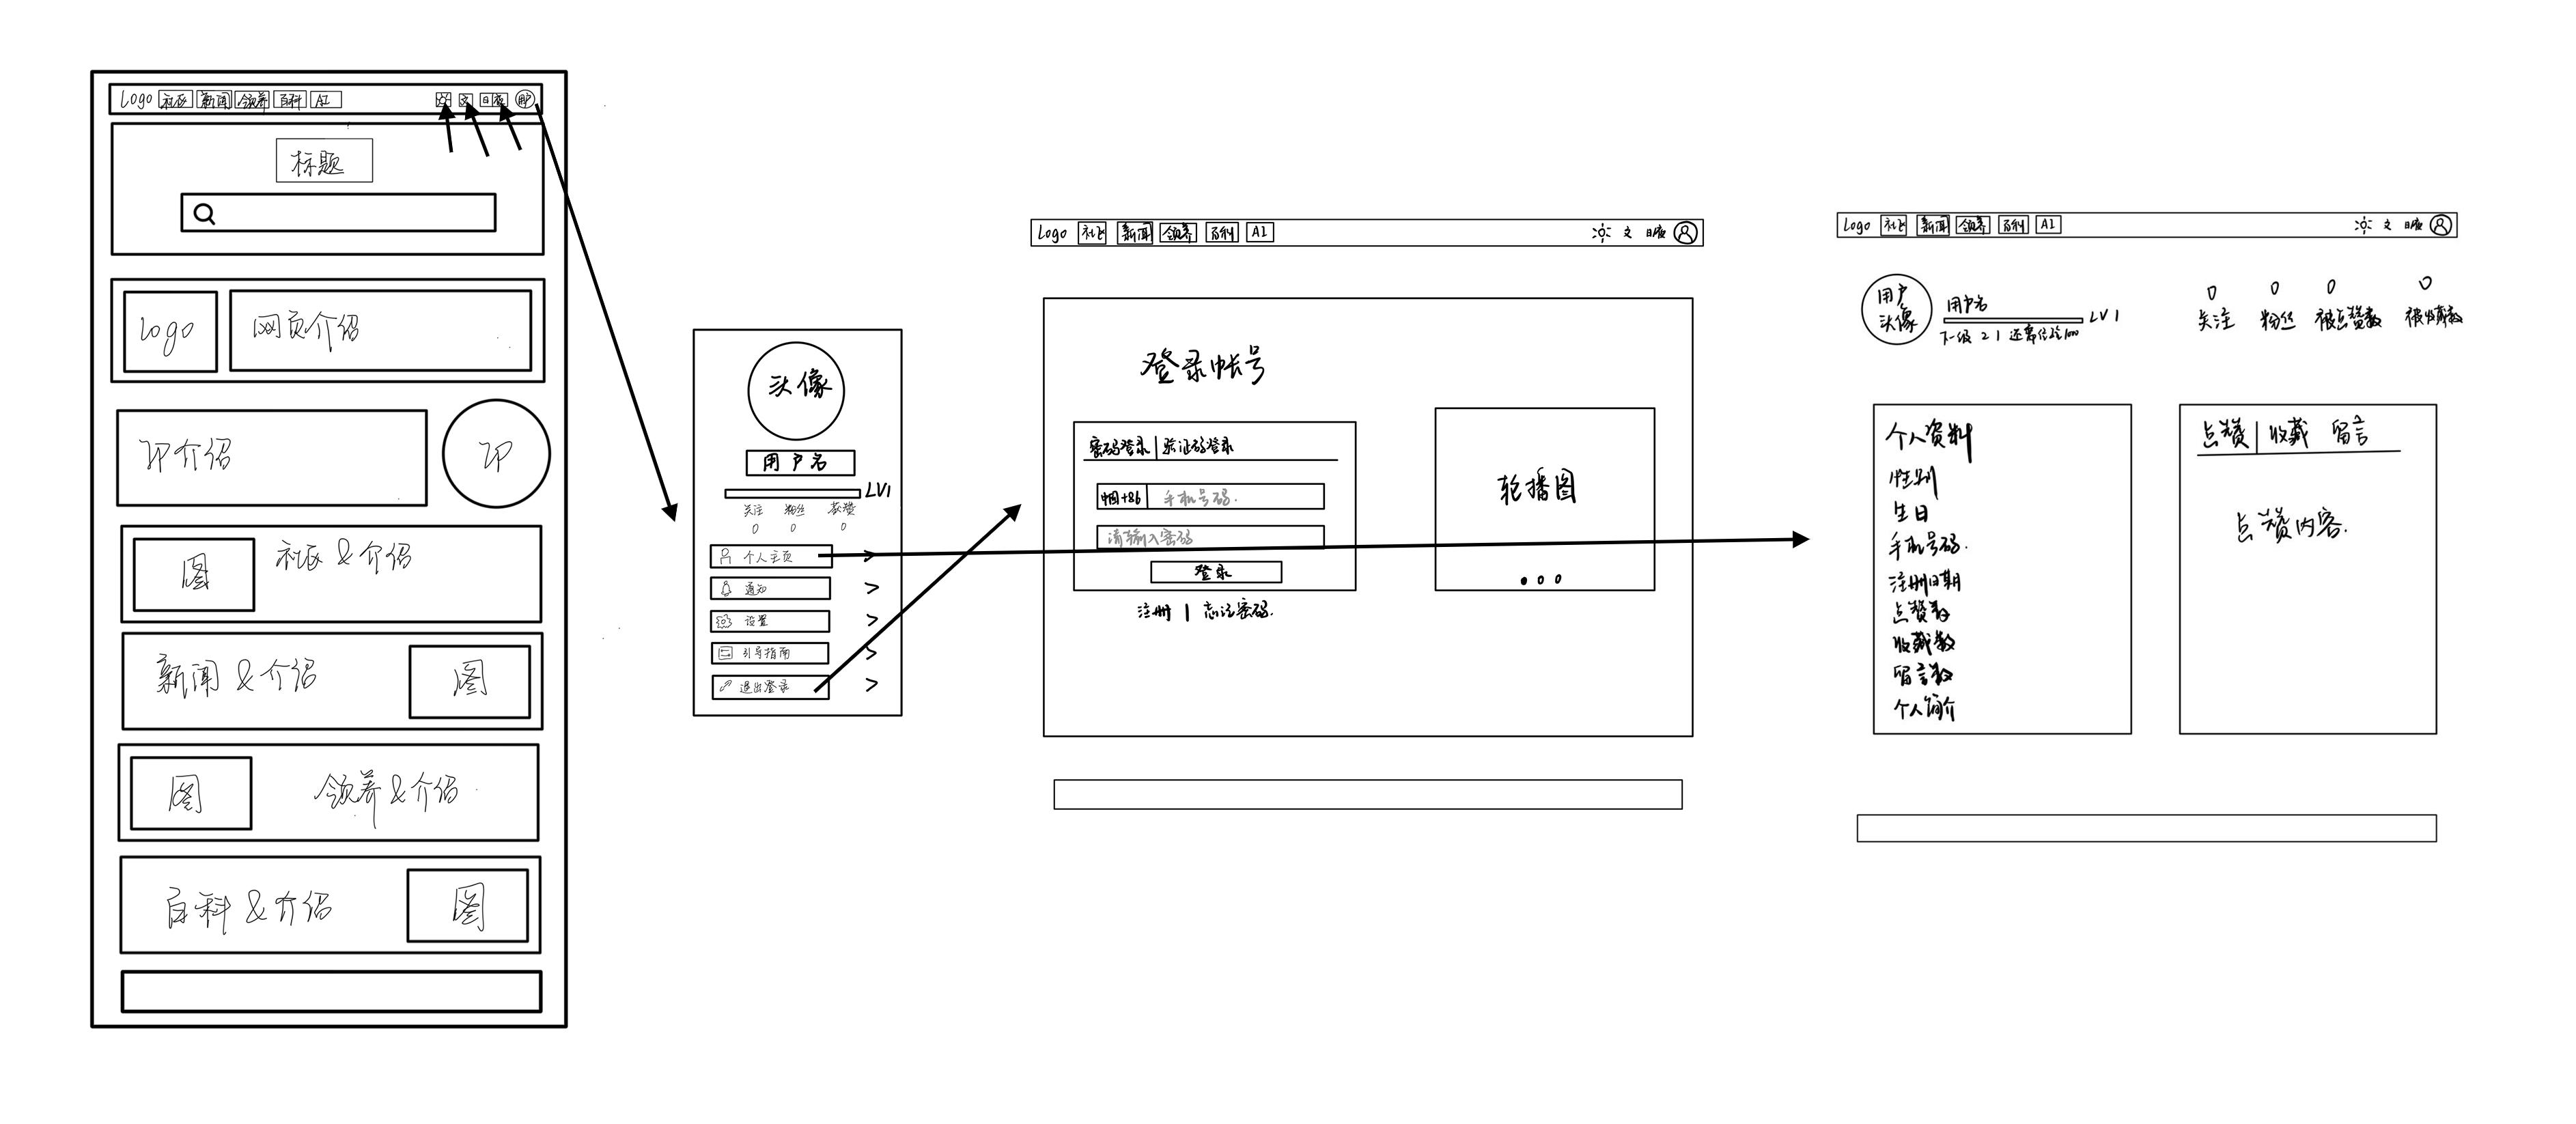
\includegraphics[scale=0.2]{UserInterfaceConceptMap.jpg}
	\caption{用户界面低保真模型}
	\label{UserInterfaceConceptMap}
\end{figure}

\begin{figure}[htbp]
	\centering
	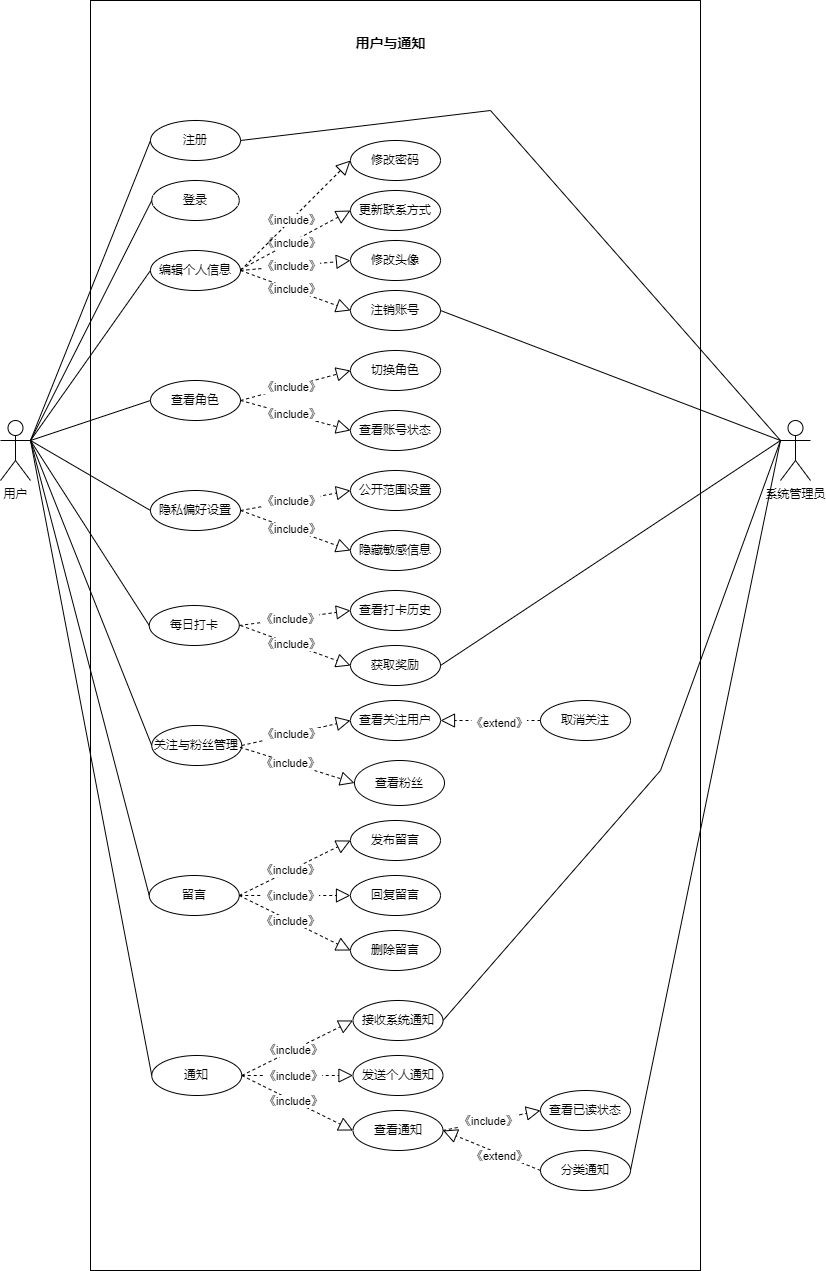
\includegraphics[scale=0.4]{UserandNotificationUseCaseDiagram.png}
	\caption{用户界面UML用例图}
	\label{UserInterfaceConceptMap}
\end{figure}

\begin{enumerate}
	\item \textbf{登录账号}:在未登录状态时,用户可以选择登录账号。通过输入手机号和密码进行登录。
	\item \textbf{进入主界面}:登录成功后,用户将进入主界面。此时,界面顶部右上角会显示用户的头像。
	\item \textbf{头像菜单操作}:当鼠标悬浮在用户头像上时,会出现一个下拉菜单,用户可以选择多种操作。点击“个人主页”可跳转到个人主页界面,查看个人资料、点赞记录、收藏内容、留言信息等。
	\item \textbf{顶部图标功能}:除了用户头像,主界面顶部右上角还会显示以下三个图标:
	\begin{itemize}
		\item \textbf{“天气”图标}:点击此图标,可以显示用户所在城市的天气信息。
		\item \textbf{“多语言切换”图标}:点击此图标,可以在包括中文、英语、俄语、德语、法语等十种语言中切换界面语言。
		\item \textbf{“深/浅色模式切换”图标}:点击此图标,可以在深色模式和浅色模式之间切换界面风格。
	\end{itemize}
\end{enumerate}

通过以上功能,用户可以方便地登录、查看个人信息,并根据需要切换语言和界面模式。

\subsubsection{宠物社区}

\begin{figure}[H]
	\centering
	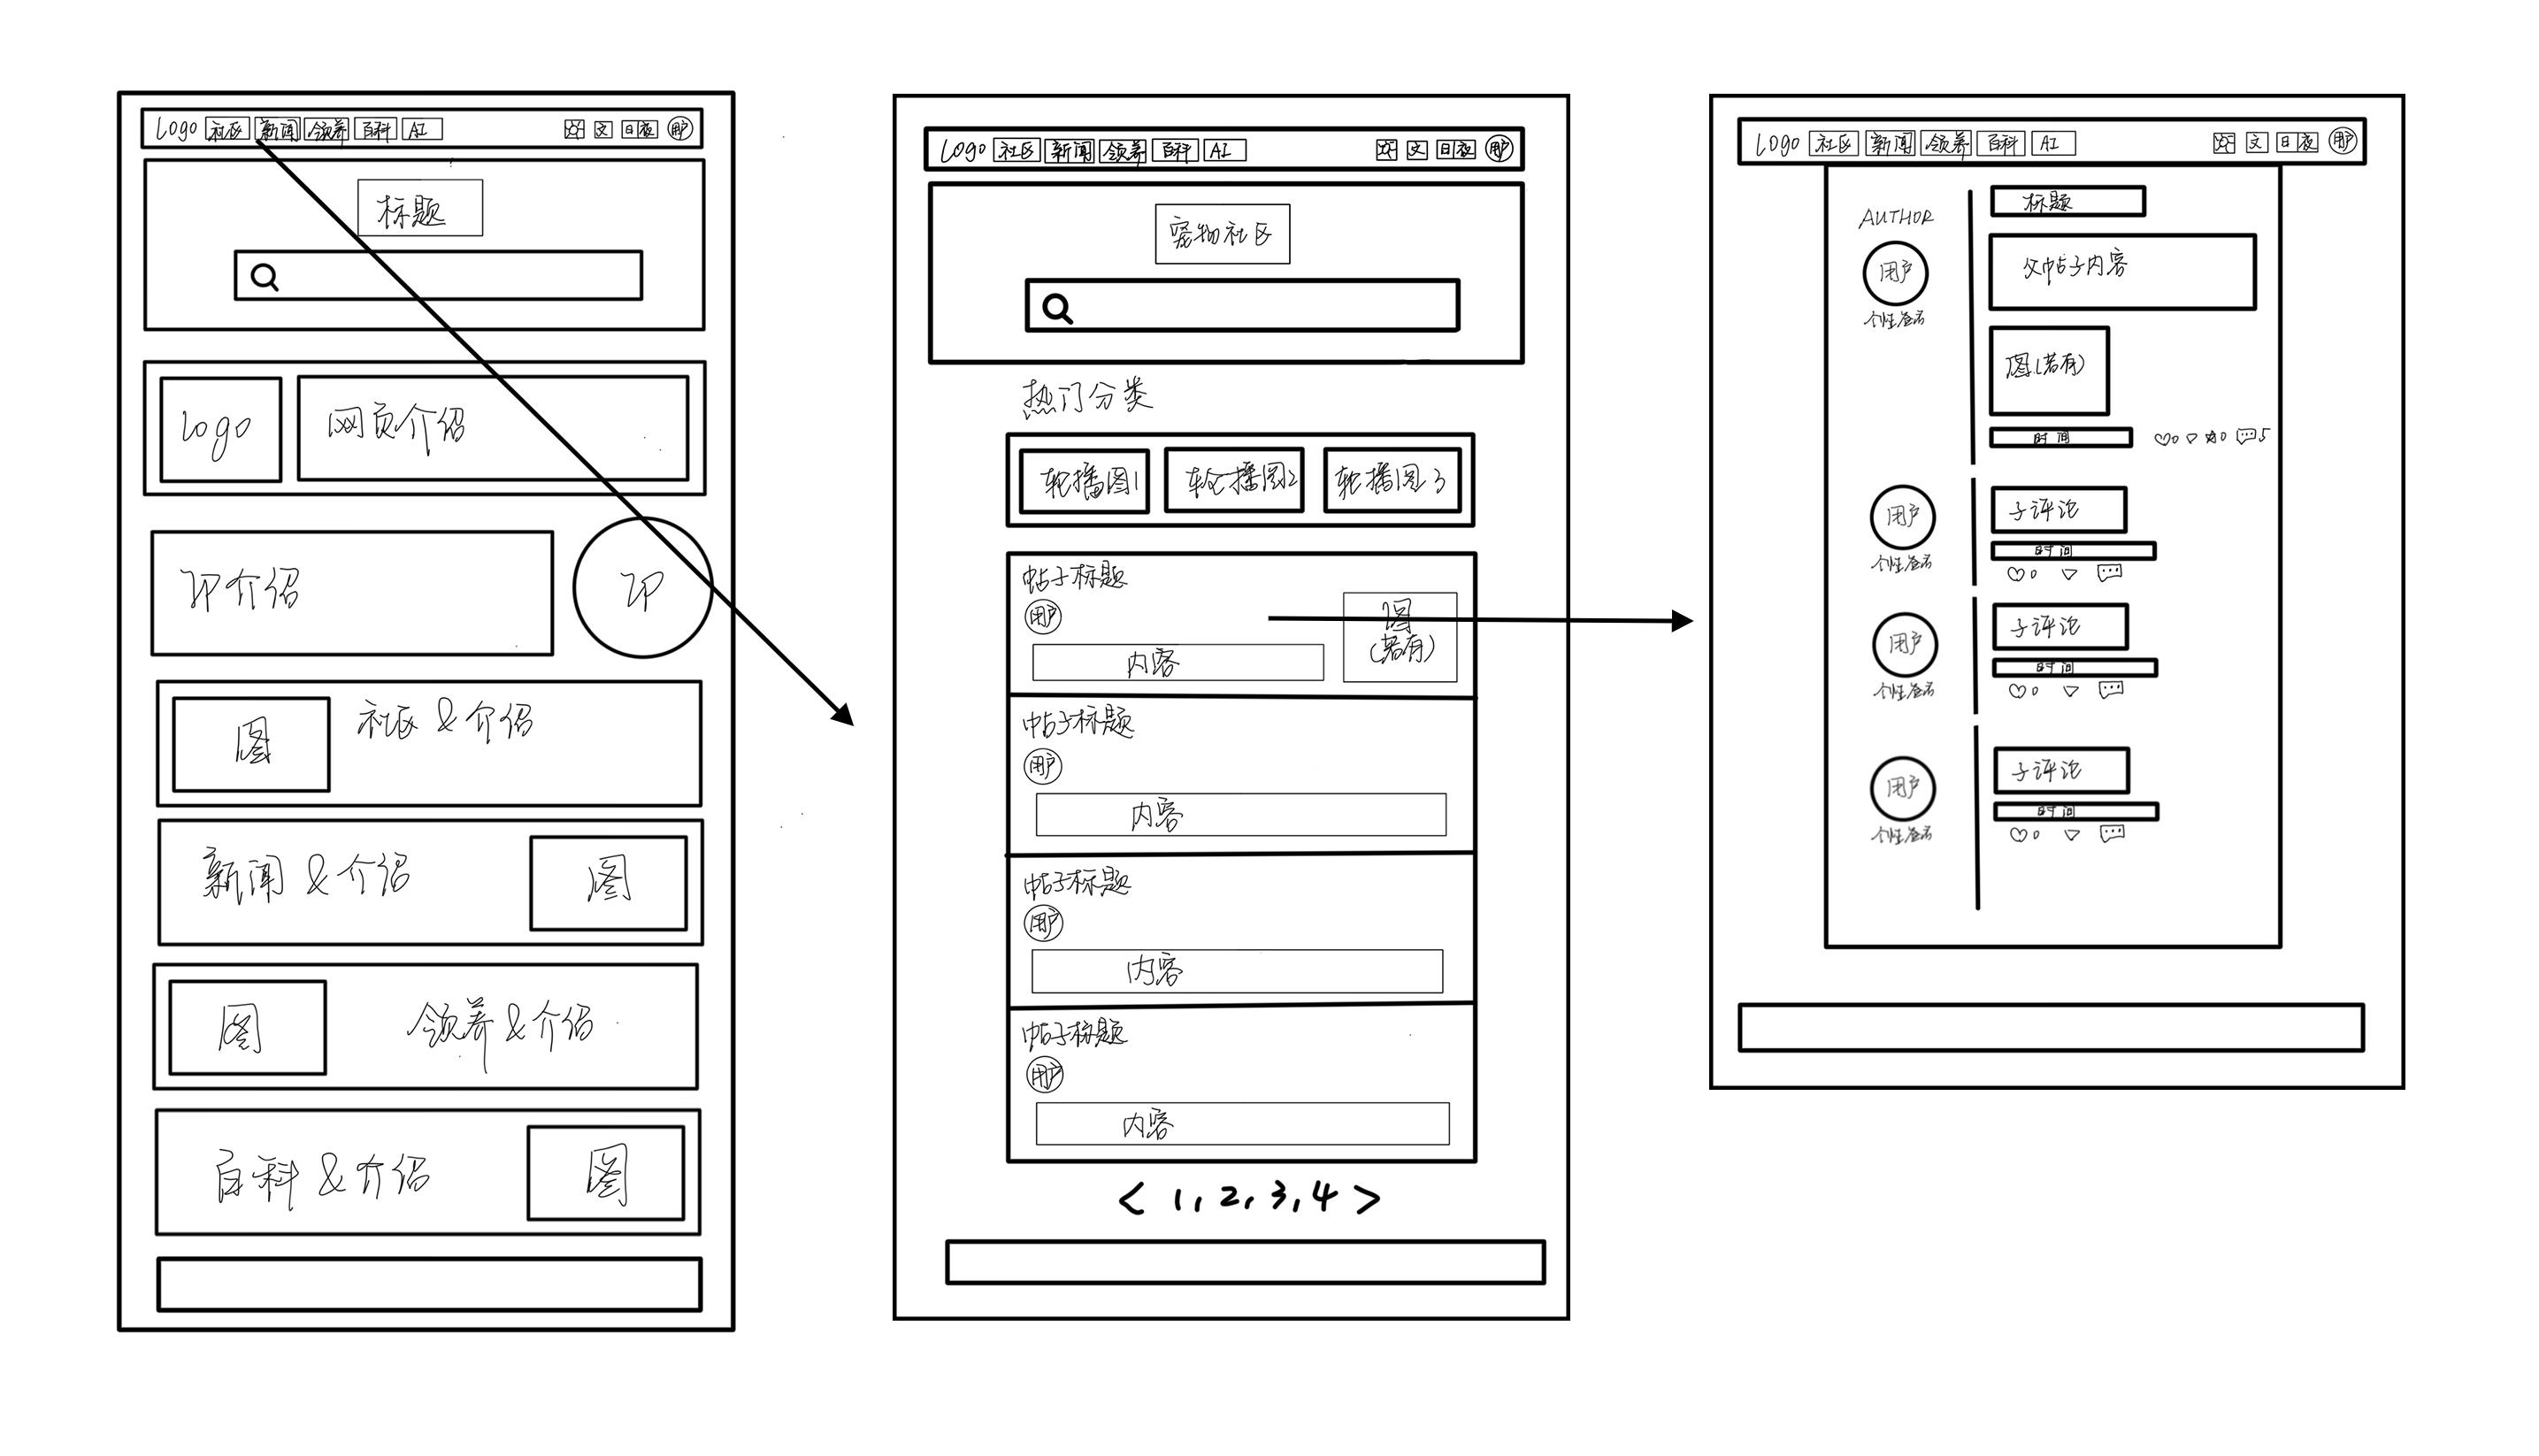
\includegraphics[scale=0.2]{PetCommunityConceptMap.jpg}
	\caption{宠物社区低保真模型}
	\label{PetCommunityConceptMap}
\end{figure}

\begin{figure}[H]
	\centering
	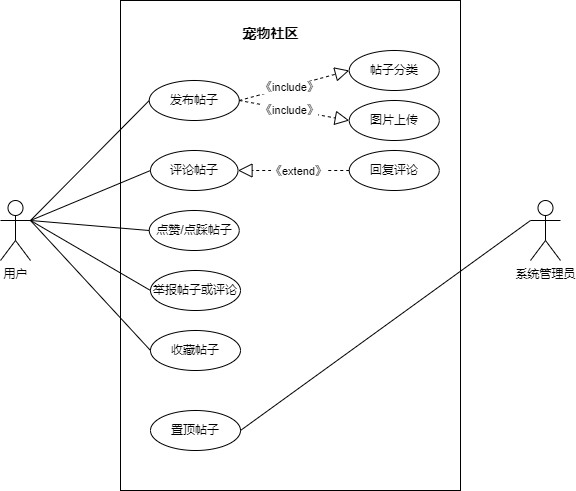
\includegraphics[scale=0.4]{PetCommunityUseCaseDiagram.png}
	\caption{宠物社区UML用例图}
	\label{UserInterfaceConceptMap}
\end{figure}

\begin{enumerate}
	\item \textbf{进入宠物社区主界面}:点击顶部导航栏中的“宠物社区”按钮,可以进入宠物社区的主界面。主界面设有搜索框,用户可以通过搜索框查询感兴趣的帖子。
	\item \textbf{浏览社区帖子分类}:在搜索框下方,展示了热门的社区帖子类别的轮播图。点击某一类别的图片,可以查看该类别下的所有社区帖子。
	\item \textbf{浏览社区帖子}:在热门的社区帖子的下方,显示了社区的所有帖子,最下方设有页面切换组件,点击可查看其他未显示的帖子。每个帖子包含标题、部分内容、图片(若存在)、帖子所属类别、点赞数、收藏数、评论数。点击帖子后,会进入该帖子详情界面,以获取更多信息。
	\item \textbf{帖子详情界面}:
	\begin{itemize}
		\item 在帖子详情界面,左侧显示了发帖人的信息,右侧显示了帖子的标题、全部内容、图片(若存在)、帖子所属类别、点赞数、收藏数、评论数。
		\item 下方为所有子评论的评论者信息与评论的具体内容,包含帖子的内容、点赞数、收藏数、评论数。
	\end{itemize}
\end{enumerate}

通过以上功能,用户可以方便地在宠物社区中查询、浏览和评论不同的帖子。

\subsubsection{宠物新闻}

\begin{figure}[H]
	\centering
	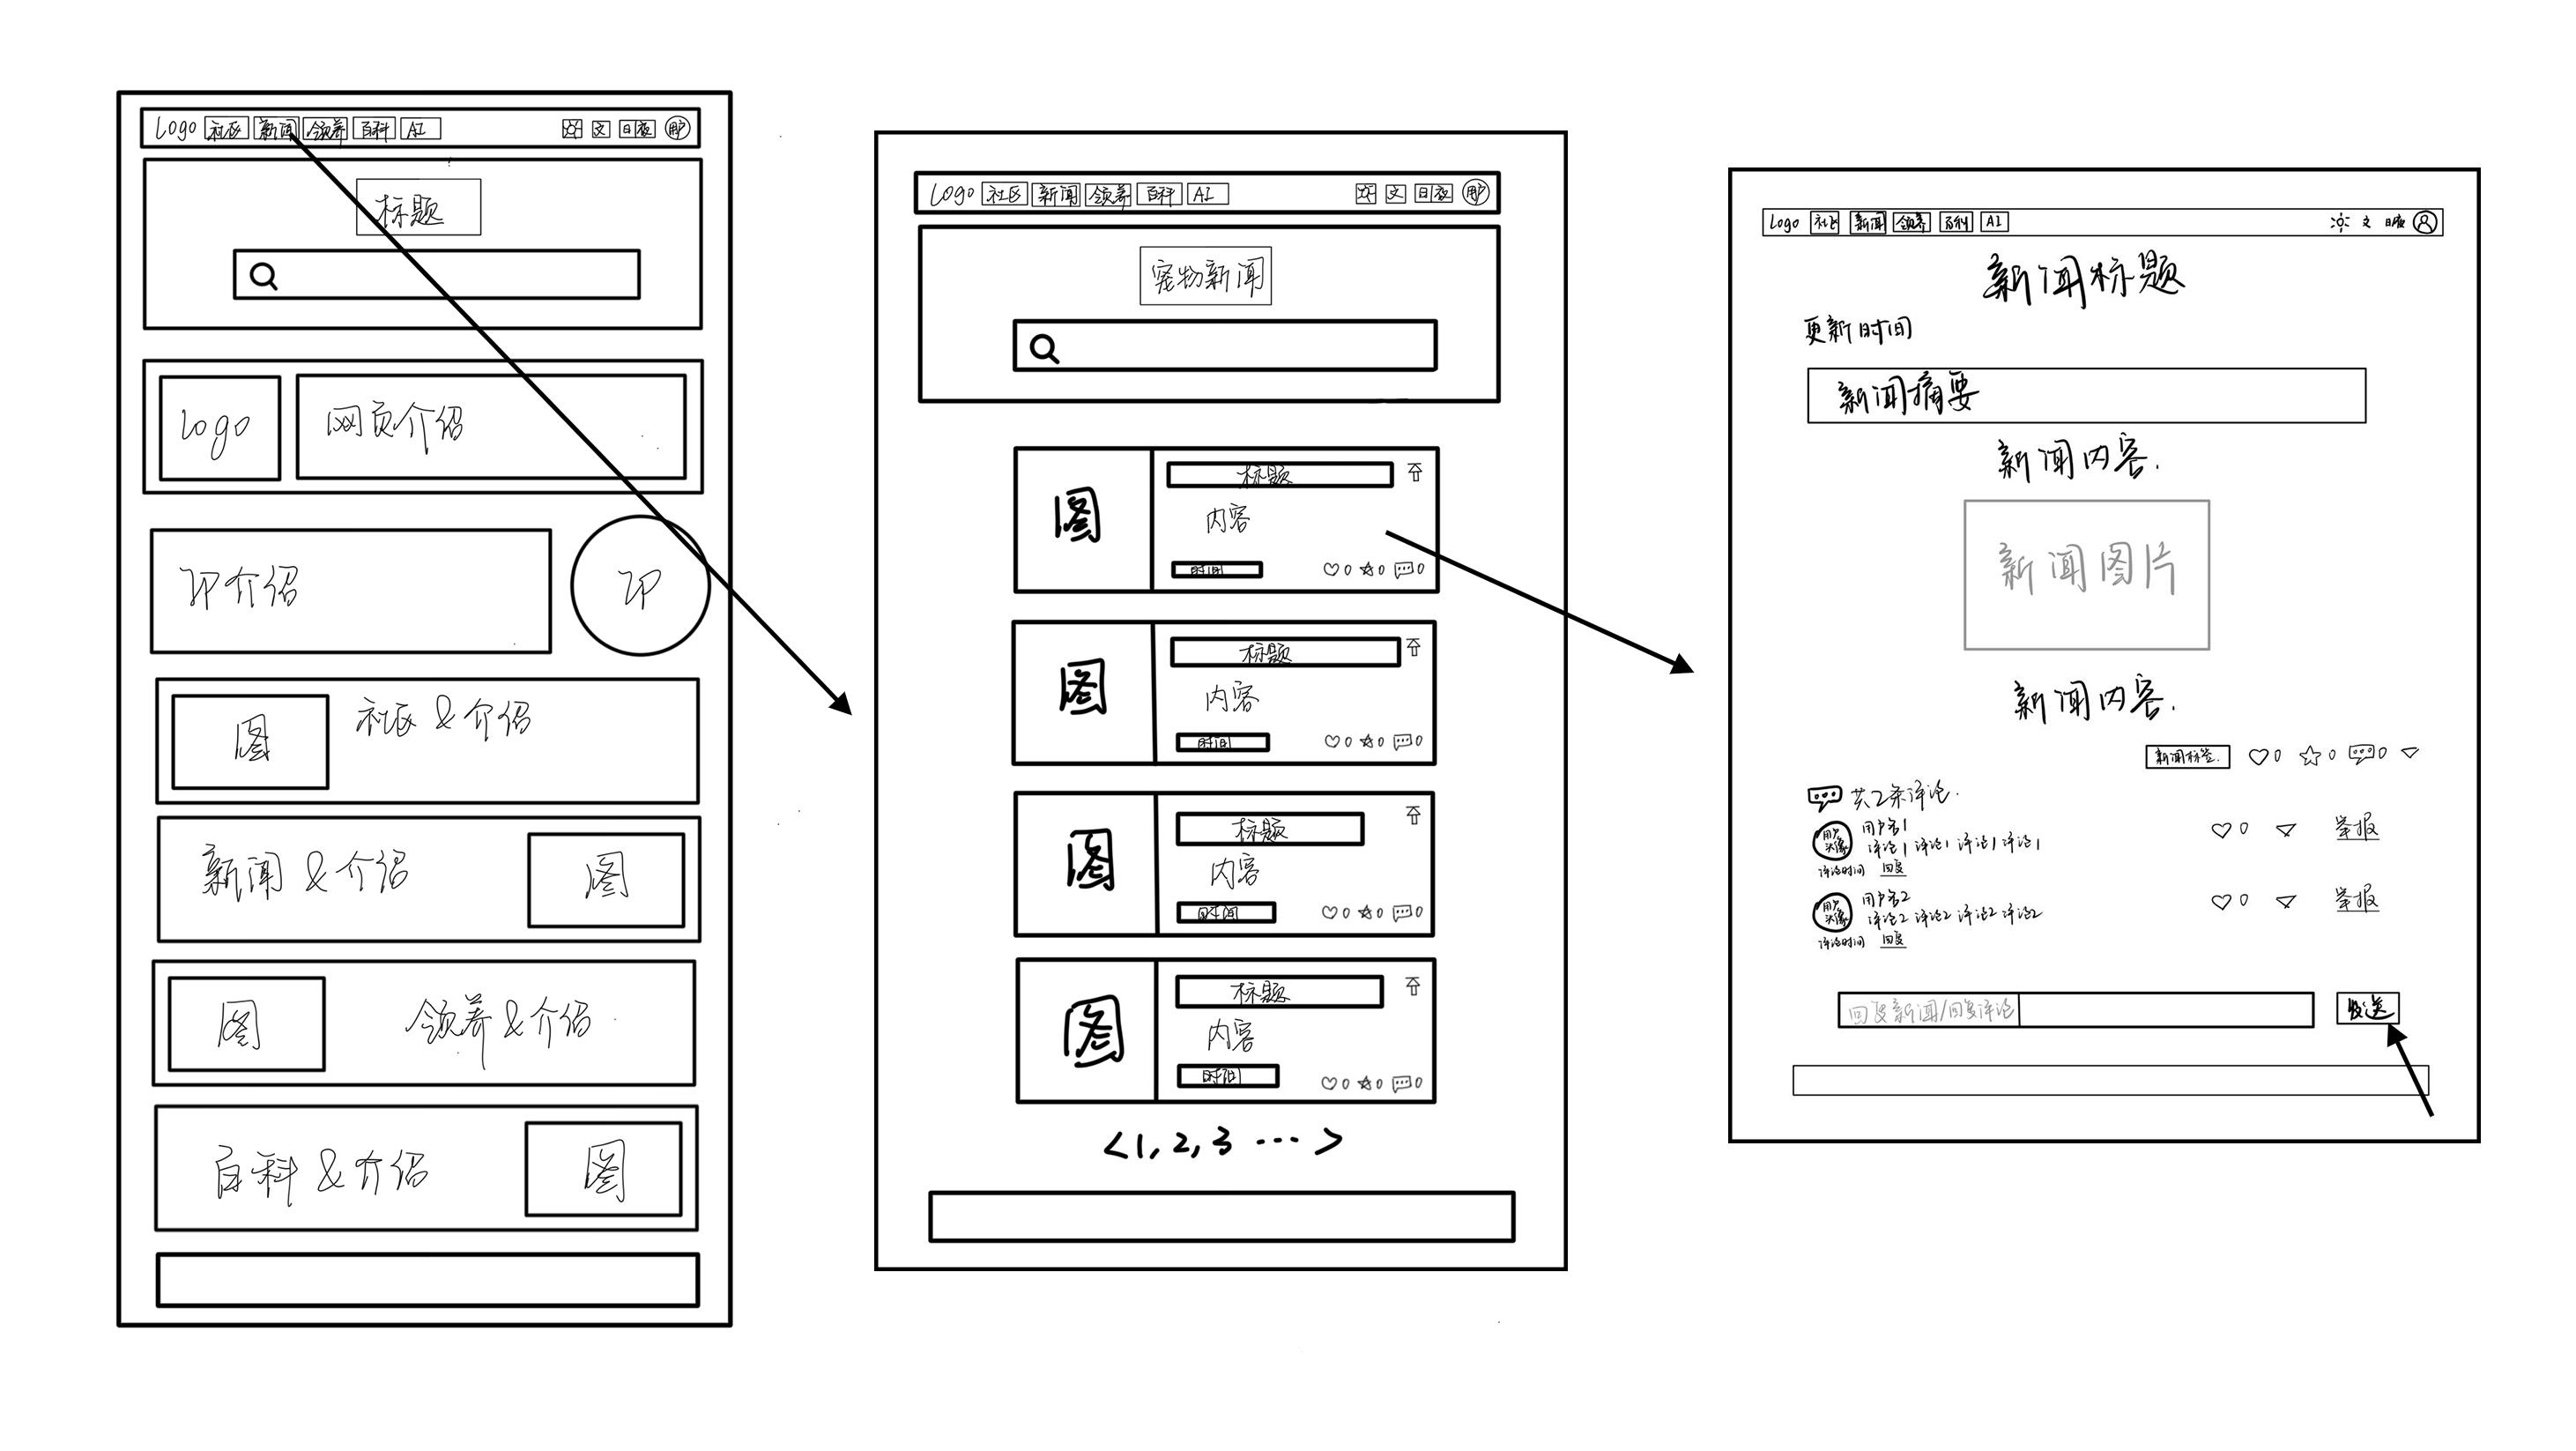
\includegraphics[scale=0.2]{PetNewsConceptMap.jpg}
	\caption{宠物新闻低保真模型}
	\label{PetNewsConceptMap}
\end{figure}

\begin{figure}[H]
	\centering
	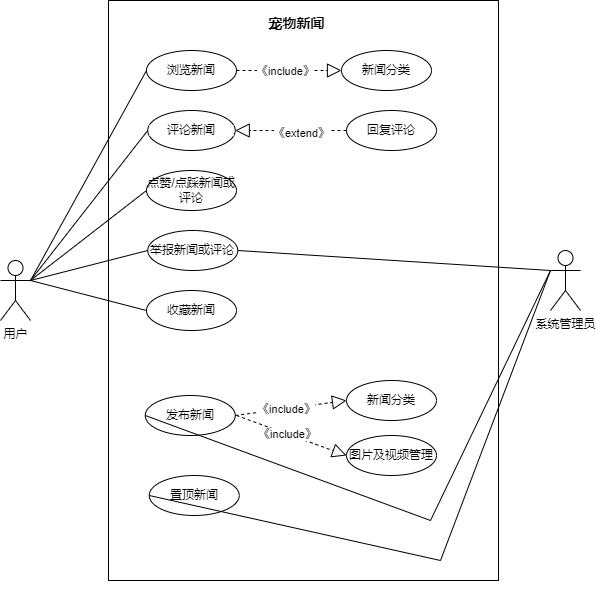
\includegraphics[scale=0.4]{PetNewsUseCaseDiagram.png}
	\caption{宠物新闻UML用例图}
	\label{UserInterfaceConceptMap}
\end{figure}

\begin{enumerate}
	\item \textbf{进入宠物新闻主界面}:点击顶部导航栏中的“宠物新闻”按钮,可以进入宠物新闻的主界面。主界面设有搜索框,用户可以通过搜索框查询感兴趣的新闻。
	\item \textbf{浏览宠物新闻}:在搜索框下方,显示了所有新闻,最下方设有页面切换组件,点击可查看其他未显示的新闻。每个新闻包含标题、部分内容、图片(若存在)、新闻所属类别、点赞数、收藏数、评论数。点击新闻后,会进入该新闻详情界面,以获取更多信息。
	\item \textbf{新闻详情界面}:
	\begin{itemize}
		\item 在新闻详情界面,显示了新闻的具体内容,包括新闻标题、时间、摘要、正文、图片(若存在)、点赞数、收藏数、评论数。
		\item 下方为所有该新闻评论者的信息与评论的具体内容,包含评论的内容、点赞数、收藏数、评论数。同时,用户可以选择在输入框输入自己对新闻的看法,并发送评论。
	\end{itemize}
\end{enumerate}

通过以上功能,用户可以方便地在宠物新闻中查询、浏览和评论不同的新闻。

\subsubsection{宠物领养}

\begin{figure}[H]
	\centering
	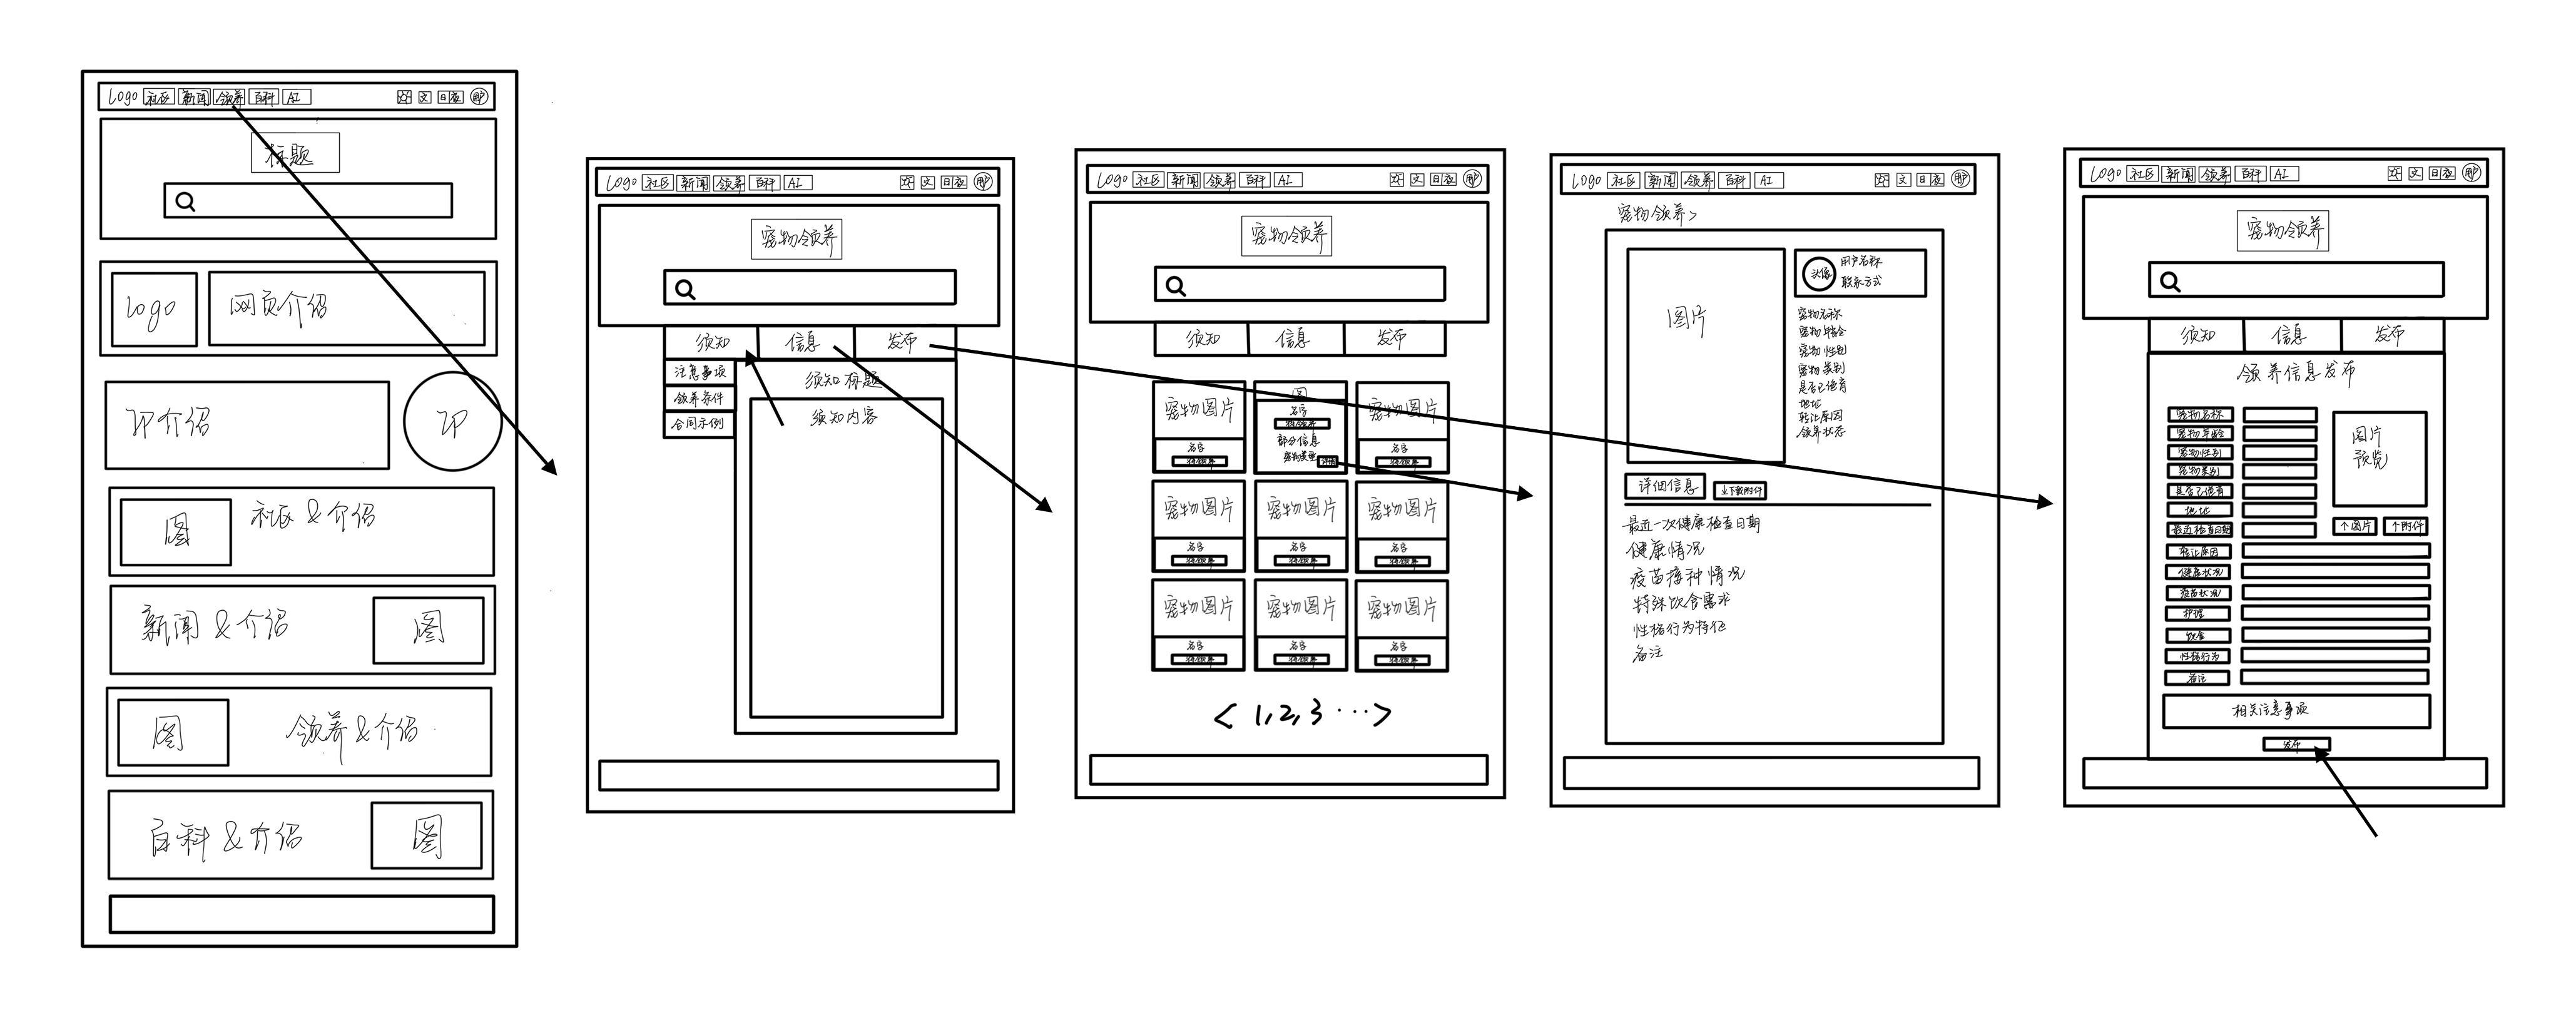
\includegraphics[scale=0.18]{PetAdoptionConceptMap.jpg}
	\caption{宠物领养低保真模型}
	\label{PetAdoptionConceptMap}
\end{figure}

\begin{figure}[H]
	\centering
	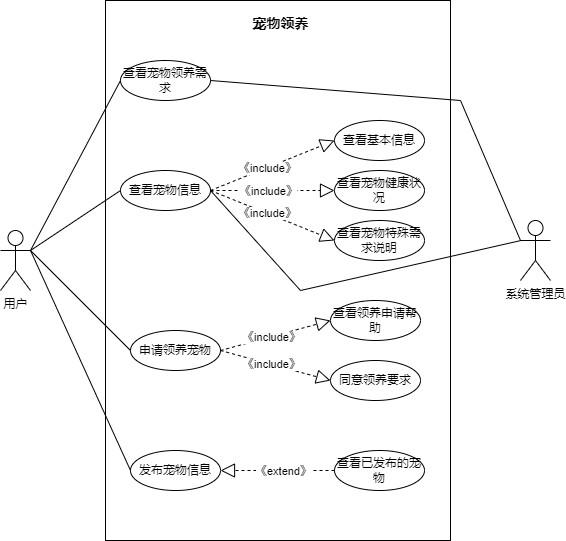
\includegraphics[scale=0.4]{PetAdoptionUseCaseDiagram.png}
	\caption{宠物领养UML用例图}
	\label{UserInterfaceConceptMap}
\end{figure}

\begin{enumerate}
	\item \textbf{进入宠物领养主界面}:点击顶部导航栏中的“宠物领养”按钮,可以进入宠物领养的主界面。主界面设有搜索框,用户可以通过搜索框查询感兴趣的内容。在搜索框下方,分别有“宠物领养须知”、“宠物领养信息”、“领养信息发布”三个功能,点击对应按钮,可以查看对应的信息。
	\item \textbf{查看宠物领养须知}:点击“宠物领养须知”,可以选择查看“宠物领养注意事项”、“宠物领养条件”、“宠物领养合同”三个文件。在“宠物领养合同”界面可以选择下载合同示例,选择下载PDF或Word版的领养合同。
	\item \textbf{浏览宠物领养信息}:点击“宠物领养信息”,可以浏览本网站所有领养宠物,包括宠物的姓名、性别、年龄、所在地以及领养状态。鼠标停留时,下方文本框上移,显示宠物类别和部分转让原因。点击“了解详情”,可以查看该宠物的详情信息。
	\item \textbf{宠物领养详情界面}:
	\begin{itemize}
		\item 在宠物详情界面,显示了该宠物的具体信息。左侧显示了宠物的图片,右侧设有发布者名片,包含用户名称和联系方式,浏览者可通过此处联系发布者。
		\item 其他宠物的具体信息,包括宠物名称、宠物年龄、宠物性别、宠物类别、是否已绝育、地址、转让原因、领养状态均显示在宠物图片右侧。其余详细信息包括最近一次健康检查日期、健康情况、疫苗接种情况、特殊饮食需求(若存在)、性格行为特征(若存在)、备注(若存在)显示在页面下方。同时,用户可以通过点击“下载附件”按钮(若存在),下载附件信息。
	\end{itemize}
	\item \textbf{领养信息发布界面}:点击“领养信息发布”,可以上传待领养宠物的相关信息。用户通过上传宠物图片、填写宠物名称、宠物年龄、宠物性别、宠物类别、是否已绝育、地址、转让原因、领养状态、最近一次健康检查日期、健康情况、疫苗接种情况、特殊饮食需求(若存在)、性格行为特征(若存在)、备注(若存在),在明确了解注意事项后,发布领养信息。
\end{enumerate}

通过以上功能,用户可以方便地在宠物领养中查询、浏览、发布领养信息。

\subsubsection{宠物百科}

\begin{figure}[H]
	\centering
	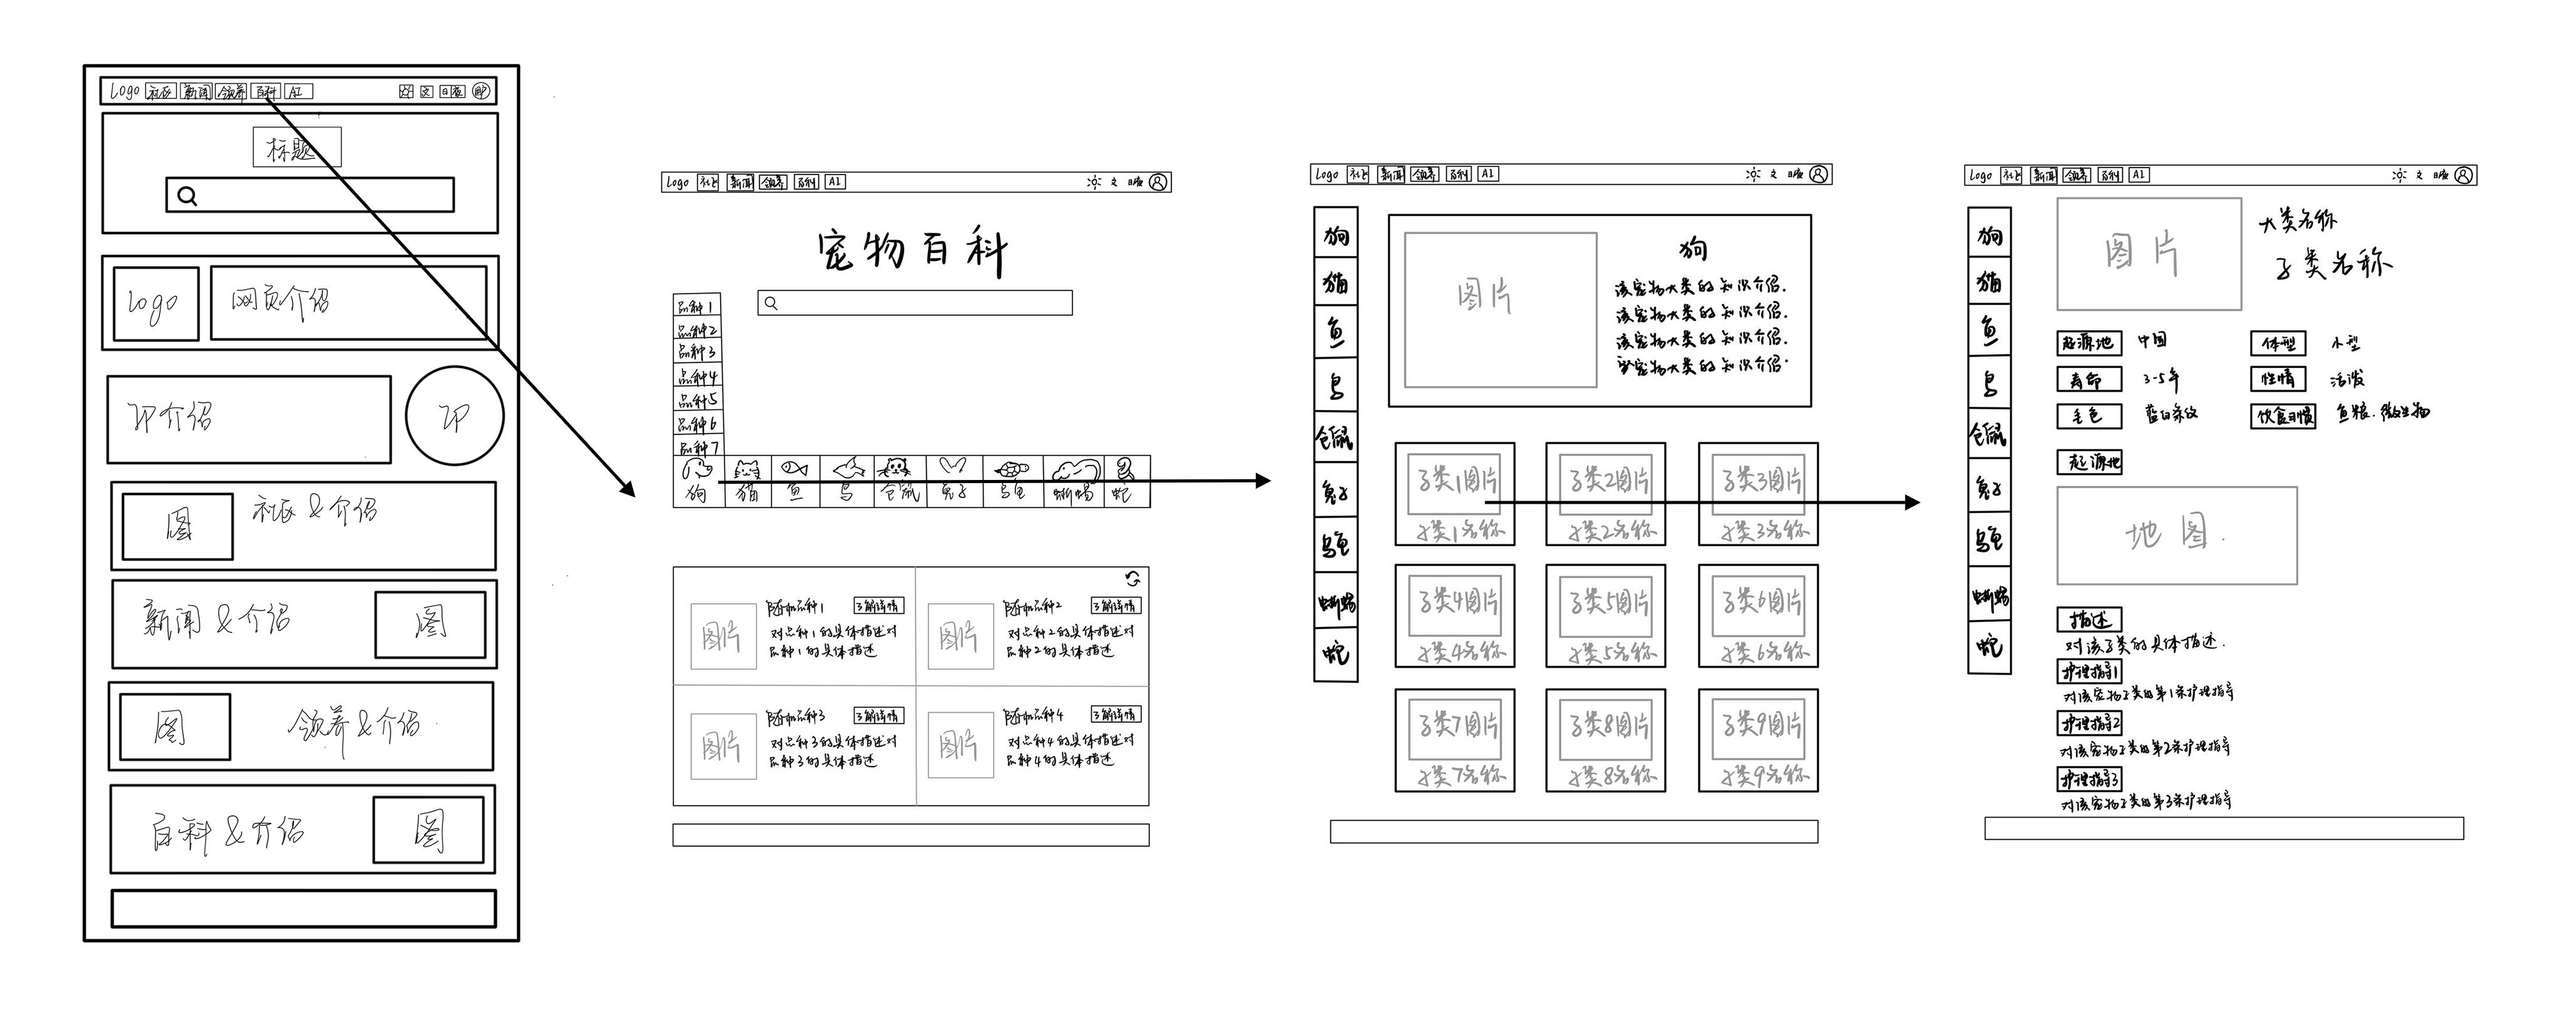
\includegraphics[scale=0.18]{PetEncyclopediaConceptMap.jpg}
	\caption{宠物百科低保真模型}
	\label{PetEncyclopediaConceptMap}
\end{figure}

\begin{figure}[H]
	\centering
	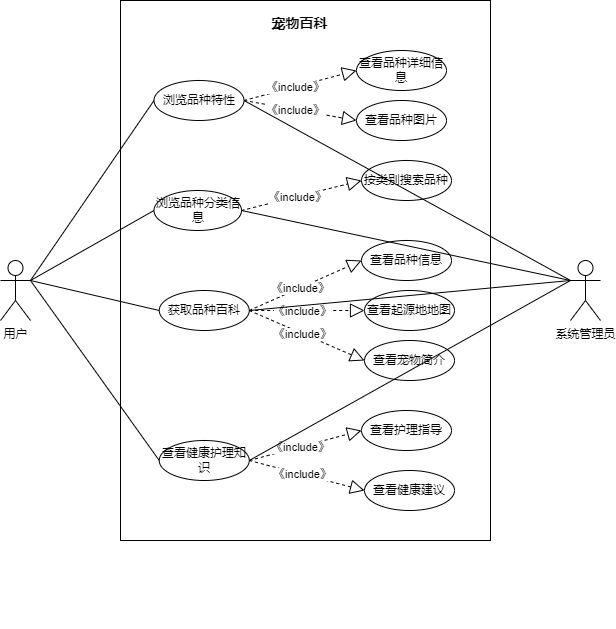
\includegraphics[scale=0.4]{PetpediaUseCaseDiagram.png}
	\caption{宠物百科UML用例图}
	\label{UserInterfaceConceptMap}
\end{figure}

\begin{enumerate}
	\item \textbf{进入宠物百科主界面}:点击顶部导航栏中的“宠物百科”按钮,可以进入宠物百科的主界面。主界面设有搜索框,用户可以通过搜索框查询感兴趣的宠物。
	\item \textbf{浏览宠物分类}:
	\begin{itemize}
		\item 在搜索框下方,展示了不同的宠物类别。点击某一类别的宠物,可以跳转到该类宠物的分类界面。
		\item 在分类界面中,可以看到该类宠物的简介及一些子类宠物的图片和名称。
		\item 当鼠标悬浮在某一类别的宠物上时,会显示该类别中的一些子类。点击具体子类的名称,可以跳转到该种宠物的子类界面,了解该种宠物的详细信息。
	\end{itemize}
	\item \textbf{随机宠物推荐}:在宠物百科主界面的下方,有随机推送的一些宠物。点击“了解详情”按钮后,会进入该种宠物的子类界面,以获取更多信息。
	\item \textbf{宠物分类界面}:
	\begin{itemize}
		\item 在宠物分类界面,左侧显示了不同的宠物大类。点击某一类宠物,可以进入对应的宠物大类界面,查看其介绍及部分子类宠物的图片和名称。
		\item 点击某个子类宠物的卡片,可以跳转到该种宠物的详情界面,进一步了解其详细信息.
	\end{itemize}
	\item \textbf{宠物子类界面}:在宠物子类界面的左侧,同样列出了不同的宠物大类。点击其中某一类宠物,可以返回到对应的宠物大类界面,了解相关信息。
\end{enumerate}

通过以上功能,用户可以方便地在宠物百科中查询和浏览不同类别及子类的宠物信息。

\subsubsection{宠物护理}

\begin{figure}[H]
	\centering
	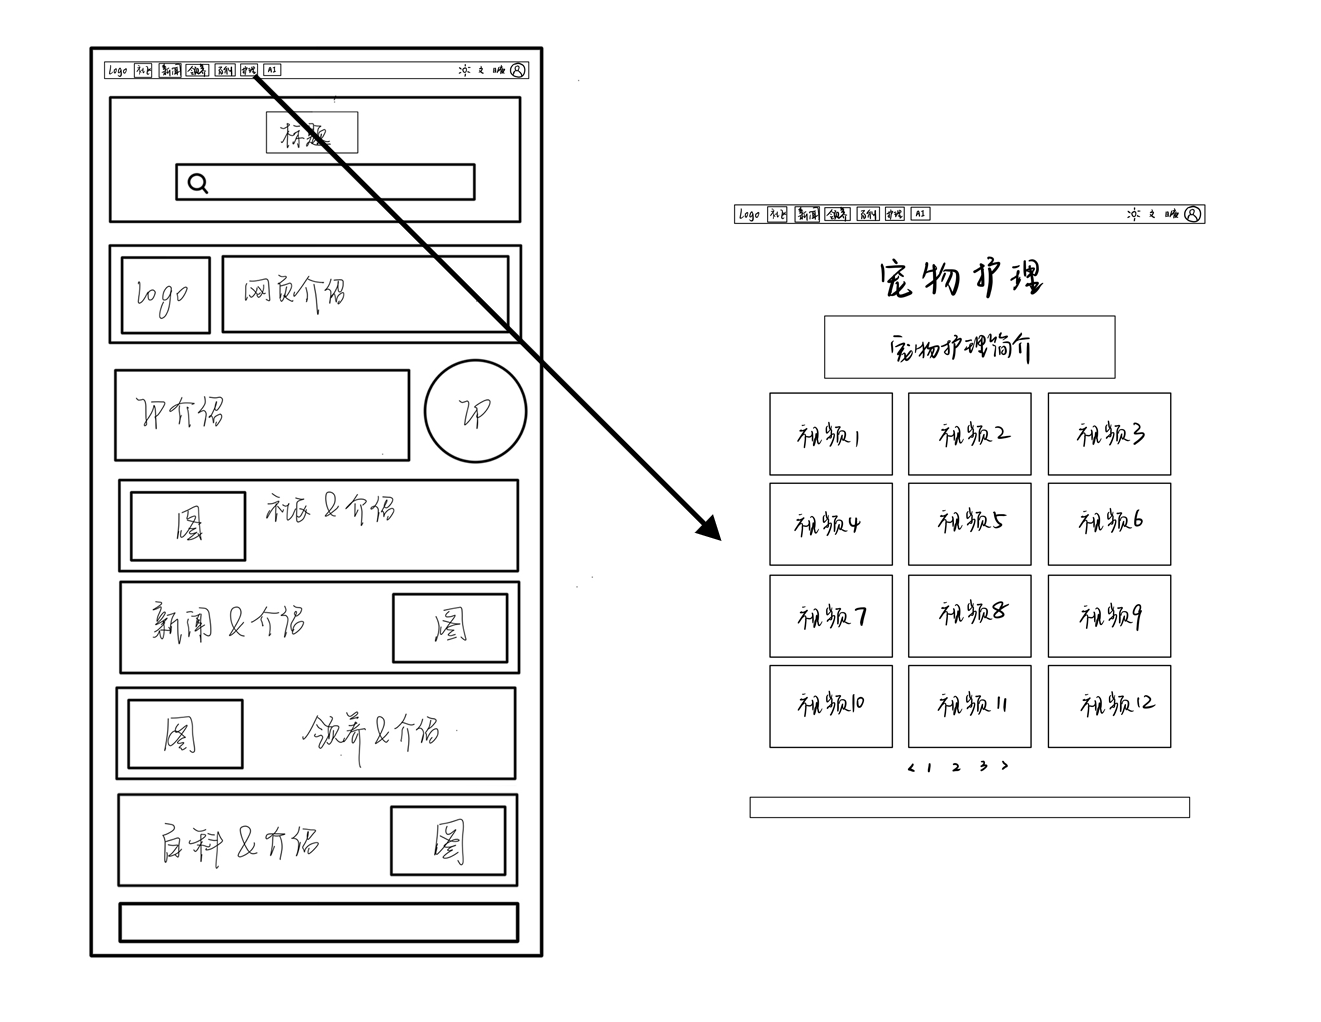
\includegraphics[scale=0.2]{PetCareConceptMap.jpg}
	\caption{宠物护理低保真模型}
	\label{PetCareConceptMap}
\end{figure}

\begin{figure}[H]
	\centering
	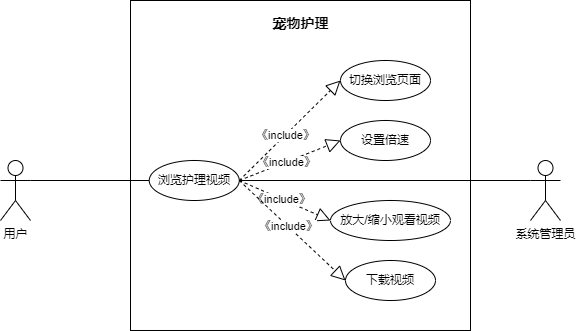
\includegraphics[scale=0.4]{PetCareUseCaseDiagram.png}
	\caption{宠物护理UML用例图}
	\label{PetCareUseCaseDiagram}
\end{figure}

\begin{enumerate}
	\item \textbf{进入宠物护理主界面}:点击顶部导航栏中的“宠物护理”按钮,可以进入宠物护理模块的主界面。主界面设有宠物护理部分的简介,帮助用户了解模块的功能和使用方式。
	\item \textbf{浏览宠物护理视频}:
	\begin{itemize}
		\item 在宠物护理界面中,将展示不同的宠物护理视频。用户可以选择感兴趣的视频并点击播放。
		\item 点击某个视频卡片后,用户可以进入该视频的播放页面,获取具体的宠物护理技巧和建议。
	\end{itemize}
	\item \textbf{视频播放}:
	\begin{itemize}
		\item 在视频播放页面,用户可以通过视频控制栏操作播放进度、调整音量、切换全屏或缩放观看。
		\item 播放过程中,用户还可以调整视频播放速度,选择适合自己的观看节奏。
	\end{itemize}
	\item \textbf{下载宠物护理视频}:用户可以选择将感兴趣的宠物护理视频下载保存,方便离线观看或日后回顾。
\end{enumerate}

通过以上功能,用户能够方便地在宠物护理模块中浏览和观看各类宠物护理相关视频,学习并掌握宠物护理技巧。

\subsubsection{宠物AI}

\begin{figure}[H]
	\centering
	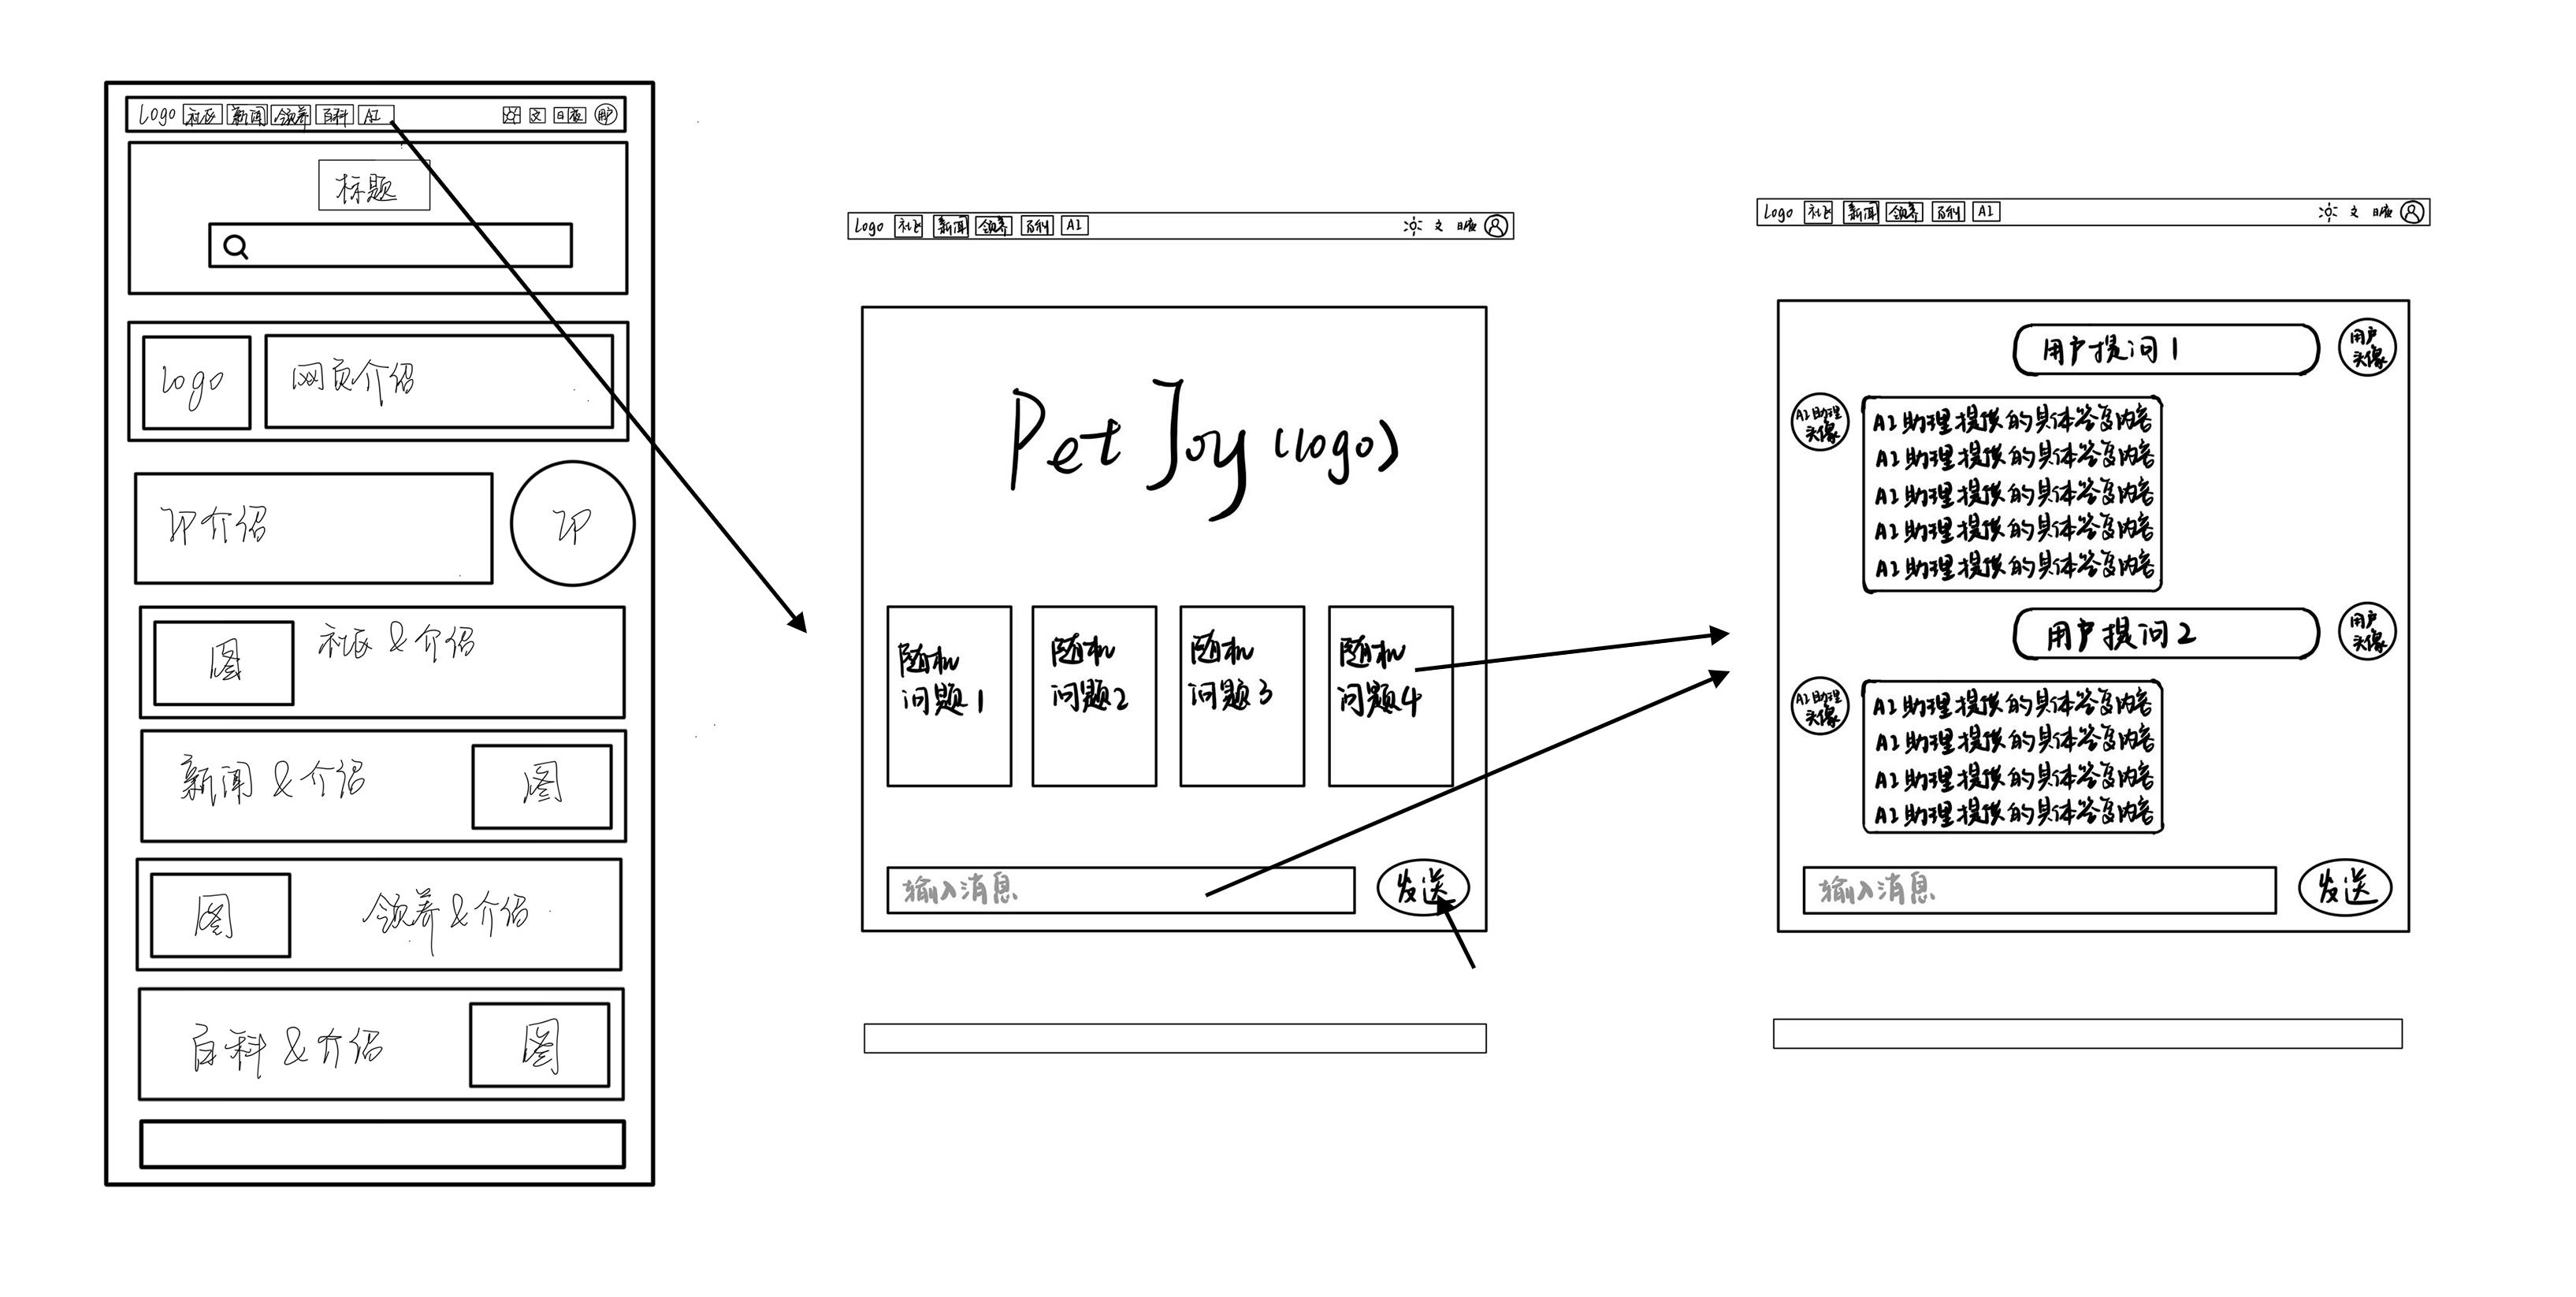
\includegraphics[scale=0.2]{PetAIConceptMap.jpg}
	\caption{宠物AI低保真模型}
	\label{PetAIConceptMap}
\end{figure}

\begin{figure}[H]
	\centering
	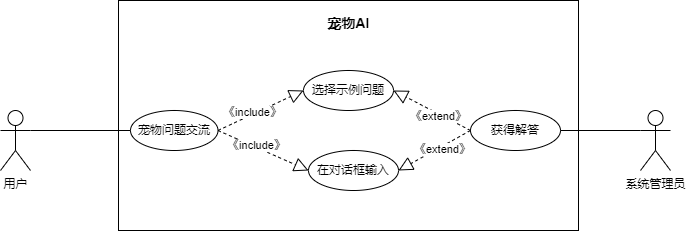
\includegraphics[scale=0.4]{PetAIUseCaseDiagram.png}
	\caption{宠物AIUML用例图}
	\label{UserInterfaceConceptMap}
\end{figure}

\begin{enumerate}
	\item \textbf{进入宠物AI主界面}:点击顶部导航栏中的“宠物AI”按钮,可以进入宠物AI的主界面。在主界面底部设有输入框,用户可以在此向AI宠物助理提出问题并发送。
	\item \textbf{常见问题快捷提问}:在输入框的上方,显示了一些常见的宠物相关问题。如果有需要,用户可以直接点击这些问题,快捷提问。
	\item \textbf{查看AI助理回答}:当用户向宠物AI助理提出问题后,界面会切换到对话界面,显示用户的提问内容以及宠物助理调用接口后生成的回答。界面设计美观,提供良好的用户体验。
\end{enumerate}

\noindent 通过以上步骤,用户可以方便地与宠物AI助理进行互动,获取关于宠物的各种信息和建议。

\subsection{用例需求分析:用户账户管理模块}

用户账户管理模块是“宠悦”平台的核心功能之一,主要涵盖用户的注册、登录、登出、注销及密码管理等操作。通过这些功能,用户能够安全、便捷地管理其账户信息,提升平台的整体用户体验。

\subsubsection{账户注册}

在用户账户管理模块中,账户注册功能帮助用户第一次使用PetJoy平台注册账号,使其能在未来更好地使用平台。

\begin{itemize}
	\item \textbf{用户注册}:用户可通过手机号验证码进行账户注册。
	\item \textbf{密码设置}:用户可根据系统提示进行个性化密码设置。
	\item \textbf{信息完善}:用户在完成密码设置后,通过输入框和选择框完善个人信息,如昵称、性别、出生日期等。
\end{itemize}

\paragraph{用户注册}

在用户账户管理模块中,用户注册是用户首次使用平台的关键步骤。该用例详细描述了用户如何通过手机验证码进行注册,以及注册过程中的各个步骤。

\begin{table}[H]
	\centering
	\caption{账户注册用例描述}
	\renewcommand\arraystretch{1.5}
	\begin{tabular}{|c|>{\raggedright\arraybackslash}p{10cm}|}
		\hline
		\textbf{名称} & \textbf{账户注册} \\ \hline
		\textbf{用例描述} & 用户通过手机号注册新账户,并通过验证码验证身份。 \\ \hline
		\textbf{参与者} & 用户 \\ \hline
		\textbf{前置条件} & 用户访问注册页面,并准备进行账户注册。 \\ \hline
		\textbf{后置条件} & 用户成功注册账户,并进入信息完善页面。 \\ \hline
		\textbf{主事件流} & 
		1. 用户输入手机号并点击获取验证码按钮。 \newline
		2. 系统发送验证码至用户手机。 \newline
		3. 用户输入收到的验证码,并点击下一步。 \newline
		4. 系统验证验证码的正确性,通过后进入密码设置页面。 \\ \hline
		\textbf{扩展事件流} & 如果验证码错误,系统提示用户重新输入。 \\ \hline
		\textbf{业务规则} & 验证码必须在规定时间内输入有效。 \\ \hline
		\textbf{备注} & 验证码的发送和验证需具备高安全性,避免恶意注册行为。 \\ \hline
	\end{tabular}
\end{table}

\paragraph{密码设置}

密码设置是用户在完成账户注册时的必要步骤,确保用户账户的安全性。

\begin{table}[H]
	\centering
	\caption{密码设置用例描述}
	\renewcommand\arraystretch{1.5}
	\begin{tabular}{|c|>{\raggedright\arraybackslash}p{10cm}|}
		\hline
		\textbf{名称} & \textbf{密码设置} \\ \hline
		\textbf{用例描述} & 用户在通过验证码验证后设置个性化密码。 \\ \hline
		\textbf{参与者} & 用户 \\ \hline
		\textbf{前置条件} & 用户已通过手机验证码验证。 \\ \hline
		\textbf{后置条件} & 密码成功设置,用户进入信息完善页面。 \\ \hline
		\textbf{主事件流} & 
		1. 用户输入个性化密码。 \newline
		2. 用户再次确认密码。 \newline
		3. 用户点击下一步按钮,系统保存密码并提示成功。 \\ \hline
		\textbf{扩展事件流} & 如果两次输入的密码不一致,系统提示用户重新输入。 \\ \hline
		\textbf{业务规则} & 密码必须符合安全规则,如长度要求、复杂性等。 \\ \hline
		\textbf{备注} & 系统应对密码进行加密存储,确保用户账户安全。 \\ \hline
	\end{tabular}
\end{table}

\paragraph{信息完善}

信息完善是用户在完成密码设置后的重要步骤,帮助系统更好地识别用户,并为用户提供个性化服务。

\begin{table}[H]
	\centering
	\caption{信息完善用例描述}
	\renewcommand\arraystretch{1.5}
	\begin{tabular}{|c|>{\raggedright\arraybackslash}p{10cm}|}
		\hline
		\textbf{名称} & \textbf{信息完善} \\ \hline
		\textbf{用例描述} & 用户在设置密码后,填写或选择个人信息,如昵称、性别、出生日期等。 \\ \hline
		\textbf{参与者} & 用户 \\ \hline
		\textbf{前置条件} & 用户已成功设置密码。 \\ \hline
		\textbf{后置条件} & 用户信息完善成功,并进入系统主页面。 \\ \hline
		\textbf{主事件流} & 
		1. 用户进入信息完善页面。 \newline
		2. 用户依次填写或选择个人信息字段。 \newline
		3. 用户确认信息无误后,点击提交按钮。 \newline
		4. 系统保存用户信息并提示成功。 \\ \hline
		\textbf{扩展事件流} & 如果某些必填信息未填写,系统提示用户补充完整。 \\ \hline
		\textbf{业务规则} & 系统应确保用户填写的信息准确,并遵循隐私保护规则。 \\ \hline
		\textbf{备注} & 用户个人信息应进行加密存储,以确保隐私安全。 \\ \hline
	\end{tabular}
\end{table}

\subsubsection{账户安全性保护}

在用户账户管理模块中,账户管理功能帮助用户维护其账户的安全和有效性。包括密码重置、账号注销等功能。

\begin{itemize}
	\item \textbf{密码重置}:用户通过验证码验证重新设置密码。
	\item \textbf{账号注销}:用户通过验证注销账号,删除相关数据。
	\item \textbf{修改绑定手机号}:用户可以更改账号绑定的手机号码。
\end{itemize}

\paragraph{密码重置}

密码重置功能确保用户在忘记密码的情况下,能够通过简单的步骤恢复访问权限。

\begin{table}[H]
	\centering
	\caption{密码重置用例描述}
	\renewcommand\arraystretch{1.5}
	\begin{tabular}{|c|>{\raggedright\arraybackslash}p{10cm}|}
		\hline
		\textbf{名称} & \textbf{密码重置} \\ \hline
		\textbf{用例描述} & 用户通过验证码验证重新设置密码。 \\ \hline
		\textbf{参与者} & 用户 \\ \hline
		\textbf{前置条件} & 用户账号绑定的手机号仍有效。 \\ \hline
		\textbf{后置条件} & 密码重置成功,用户可使用新密码登录。 \\ \hline
		\textbf{主事件流} & 
		1. 用户输入账号绑定的手机号并点击获取验证码。 \newline
		2. 用户输入收到的验证码并设置新密码。 \\ \hline
		\textbf{扩展事件流} & 如果验证码错误,系统提示用户重新输入。 \\ \hline
		\textbf{业务规则} & 验证码必须在规定时间内输入有效。 \\ \hline
		\textbf{备注} & 系统应提示用户设置高强度密码以增强安全性。 \\ \hline
	\end{tabular}
\end{table}

\paragraph{账号注销}

账号注销功能允许用户在不再需要使用平台时,彻底删除其账户及相关数据。

\begin{table}[H]
	\centering
	\caption{账号注销用例描述}
	\renewcommand\arraystretch{1.5}
	\begin{tabular}{|c|>{\raggedright\arraybackslash}p{10cm}|}
		\hline
		\textbf{名称} & \textbf{账号注销} \\ \hline
		\textbf{用例描述} & 用户在个人页面中选择注销账号,并通过验证后执行注销操作。 \\ \hline
		\textbf{参与者} & 用户 \\ \hline
		\textbf{前置条件} & 用户账号绑定的手机号仍有效。 \\ \hline
		\textbf{后置条件} & 账号及相关数据被删除,用户无法再使用此账号登录。 \\ \hline
		\textbf{主事件流} & 
		1. 用户输入账号绑定的手机号并进行验证码验证。 \newline
		2. 用户阅读并确认注销注意事项。 \newline
		3. 用户点击确认按钮,执行注销操作。 \\ \hline
		\textbf{扩展事件流} & 如果用户在注销前改变主意,系统允许取消注销操作。 \\ \hline
		\textbf{业务规则} & 注销操作不可逆,需确保用户已确认其后果。 \\ \hline
		\textbf{备注} & 系统需保留一段时间内的数据备份,以防误操作。 \\ \hline
	\end{tabular}
\end{table}

\paragraph{修改绑定手机号}

修改绑定手机号功能允许用户更改账号绑定的手机号码,确保账号信息的准确性。

\begin{table}[H]
	\centering
	\caption{修改绑定手机号用例描述}
	\renewcommand\arraystretch{1.5}
	\begin{tabular}{|c|>{\raggedright\arraybackslash}p{10cm}|}
		\hline
		\textbf{名称} & \textbf{修改绑定手机号} \\ \hline
		\textbf{用例描述} & 用户在个人页面中选择修改绑定手机号,并通过验证后执行修改操作。 \\ \hline
		\textbf{参与者} & 用户 \\ \hline
		\textbf{前置条件} & 用户账号绑定的手机号仍有效。 \\ \hline
		\textbf{后置条件} & 手机号修改成功,用户可使用新手机号登录。 \\ \hline
		\textbf{主事件流} & 
		1. 用户输入新旧手机号并点击获取验证码。 \newline
		2. 用户输入收到的验证码并进行验证。 \newline
		3. 用户点击确认按钮,执行手机号修改操作。 \\ \hline
		\textbf{扩展事件流} & 如果验证码错误,系统提示用户重新输入。 \\ \hline
		\textbf{业务规则} & 验证码必须在规定时间内输入有效。 \\ \hline
		\textbf{备注} & 系统应提示用户确保新手机号的准确性。 \\ \hline
	\end{tabular}
\end{table}

\subsubsection{账号登陆管理}

在账号管理模块中,用户登录和登出是核心功能之一。这些功能确保用户能够安全地访问系统,并在使用后正确退出。该模块涵盖了不同的登录方式、登出操作以及人类测试,保证了系统的安全性和用户的便捷性。

\begin{itemize}
	\item \textbf{账号登录选择}:用户在系统未登录状态下,可以选择验证码登录或账户密码登录。这一功能提供了灵活的登录方式,用户可以根据个人偏好和实际情况选择合适的登录方式。
	\item \textbf{账号登出}:用户在已登录的系统中可以随时选择登出操作。这一功能确保用户能够在使用完系统后安全退出,防止账户被他人滥用。
	\item \textbf{验证码登录}:用户通过手机号码获取验证码进行登录。这一功能增加了登录过程的安全性,防止密码被破解或滥用。
	\item \textbf{密码登录}:用户通过账户绑定的密码进行直接登录。这一功能为用户提供了快速登录的方式,但也需要确保密码的安全性。
	\item \textbf{人类测试}:系统对每个新登录的用户进行人类测试,以防止恶意脚本登录。这一功能有效地维护了平台的安全性和秩序。
\end{itemize}

\paragraph{账号登录选择}

在账号登录选择功能中,用户可以在系统的主页或注册页面点击登录按钮,以选择验证码登录或账户密码登录。下表详细描述了该用例的各项需求,包括用例名称、描述、参与者、前置条件、后置条件、主事件流、扩展事件流、业务规则及备注。
\begin{table}[H]
	\centering
	\caption{账号登录选择用例描述}
	\renewcommand\arraystretch{1.5}
	\begin{tabular}{|c|>{\raggedright\arraybackslash}p{10cm}|}
		\hline
		\textbf{名称} & \textbf{账号登录选择} \\ \hline
		\textbf{用例描述} & 用户在未登录系统时,可以选择验证码登录或账户密码登录。该功能允许用户根据自己的需求选择合适的登录方式。 \\ \hline
		\textbf{参与者} & 主要参与者: 用户 \\ \hline
		\textbf{前置条件} & 用户在未登录的系统主页或注册页面。 \\ \hline
		\textbf{后置条件} & 用户选择登录方式后,系统将引导用户进入对应的登录页面。 \\ \hline
		\textbf{主事件流} & 
		1. 用户点击登录按钮。 \newline
		2. 系统展示选择验证码登录或账户密码登录的选项。 \newline
		3. 用户选择所需的登录方式。 \newline
		4. 系统引导用户进入选择的登录页面。 \\ \hline
		\textbf{扩展事件流} & 如果用户选择了未支持的登录方式,则系统提示用户选择有效的登录方式。 \\ \hline
		\textbf{业务规则} & 用户只能选择支持的登录方式,系统应确保所有选择的方式正常工作。 \\ \hline
		\textbf{备注} & 系统应提供清晰的登录方式选择界面,方便用户操作。 \\ \hline
	\end{tabular}
\end{table}

\paragraph{账号登出}

在账号登出功能中,用户可以通过点击头像下拉菜单中的登出按钮来退出系统。下表详细列出了该用例的各项需求,包括功能描述、参与者角色、操作流程及相关规则。

\begin{table}[H]
	\centering
	\caption{账号登出用例描述}
	\renewcommand\arraystretch{1.5}
	\begin{tabular}{|c|>{\raggedright\arraybackslash}p{10cm}|}
		\hline
		\textbf{名称} & \textbf{账号登出} \\ \hline
		\textbf{用例描述} & 用户在已登录系统中,通过点击头像下拉菜单中的登出按钮来退出账号。 \\ \hline
		\textbf{参与者} & 主要参与者: 用户 \\ \hline
		\textbf{前置条件} & 用户已经登录系统。 \\ \hline
		\textbf{后置条件} & 用户成功退出系统,返回到未登录状态。 \\ \hline
		\textbf{主事件流} & 
		1. 用户点击头像框,展开下拉菜单。 \newline
		2. 用户点击“登出”按钮。 \newline
		3. 系统处理登出请求,用户被引导回到未登录状态。 \\ \hline
		\textbf{扩展事件流} & 如果登出操作失败,则系统提示用户重新尝试登出。 \\ \hline
		\textbf{业务规则} & 用户登出后,系统应清除所有会话信息,确保账户安全。 \\ \hline
		\textbf{备注} & 系统应提供确认退出提示,以防用户误操作。 \\ \hline
	\end{tabular}
\end{table}

\paragraph{验证码登录}

在验证码登录功能中,用户选择通过手机号码获取验证码进行登录。下表详细描述了该用例的各项需求,包括功能描述、参与者角色、操作流程及相关规则。

\begin{table}[H]
	\centering
	\caption{验证码登录用例描述}
	\renewcommand\arraystretch{1.5}
	\begin{tabular}{|c|>{\raggedright\arraybackslash}p{10cm}|}
		\hline
		\textbf{名称} & \textbf{验证码登录} \\ \hline
		\textbf{用例描述} & 用户通过输入手机号码获取验证码进行登录,系统通过验证码验证用户身份。 \\ \hline
		\textbf{参与者} & 主要参与者: 用户 \\ \hline
		\textbf{前置条件} & 用户在登录页面,且系统支持验证码登录。 \\ \hline
		\textbf{后置条件} & 用户成功登录系统,系统进行人类测试。 \\ \hline
		\textbf{主事件流} & 
		1. 系统提示用户输入手机号码。 \newline
		2. 用户输入手机号码并点击“获取验证码”按钮。 \newline
		3. 用户输入收到的验证码。 \newline
		4. 用户点击“登录”按钮。 \newline
		5. 系统验证验证码并完成用户登录。 \\ \hline
		\textbf{扩展事件流} & 如果验证码输入错误,系统提示用户重新输入。 \\ \hline
		\textbf{业务规则} & 验证码有效期应有限制,系统应确保验证码的安全性。 \\ \hline
		\textbf{备注} & 系统应支持验证码重发功能,避免用户因验证码丢失无法登录。 \\ \hline
	\end{tabular}
\end{table}

\paragraph{密码登录}

在密码登录功能中,用户通过输入账户绑定的密码直接登录系统。下表详细列出了该用例的各项需求,包括功能描述、参与者角色、操作流程及相关规则。

\begin{table}[H]
	\centering
	\caption{密码登录用例描述}
	\renewcommand\arraystretch{1.5}
	\begin{tabular}{|c|>{\raggedright\arraybackslash}p{10cm}|}
		\hline
		\textbf{名称} & \textbf{密码登录} \\ \hline
		\textbf{用例描述} & 用户通过输入账户绑定的密码直接登录系统,系统验证密码的正确性。 \\ \hline
		\textbf{参与者} & 主要参与者: 用户 \\ \hline
		\textbf{前置条件} & 用户在登录页面,且系统支持密码登录。 \\ \hline
		\textbf{后置条件} & 用户成功登录系统,系统进行人类测试。 \\ \hline
		\textbf{主事件流} & 
		1. 系统提示用户输入手机号。 \newline
		2. 用户输入手机号及对应的密码。 \newline
		3. 用户点击“登录”按钮。 \newline
		4. 系统验证密码并完成用户登录。 \\ \hline
		\textbf{扩展事件流} & 如果密码错误,系统提示用户重新输入。 \\ \hline
		\textbf{业务规则} & 系统应支持密码重置功能,确保用户能够恢复账户访问权限。 \\ \hline
		\textbf{备注} & 系统应支持用户更改密码功能,并提供密码强度检测。 \\ \hline
	\end{tabular}
\end{table}

\paragraph{人类测试}

在人类测试功能中,系统对每个新登录的用户进行验证,以防止恶意脚本登录。下表详细描述了该用例的各项需求,包括功能描述、参与者角色、操作流程及相关规则。

\begin{table}[H]
	\centering
	\caption{人类测试用例描述}
	\renewcommand\arraystretch{1.5}
	\begin{tabular}{|c|>{\raggedright\arraybackslash}p{10cm}|}
		\hline
		\textbf{名称} & \textbf{人类测试} \\ \hline
		\textbf{用例描述} & 系统对每个新登录的用户进行人类测试,以防止恶意脚本登录。 \\ \hline
		\textbf{参与者} & 主要参与者: 用户 \\ \hline
		\textbf{前置条件} & 用户完成登录流程并成功进入系统。 \\ \hline
		\textbf{后置条件} & 用户完成测试并成功访问系统。 \\ \hline
		\textbf{主事件流} & 
		1. 系统检测到新用户登录。 \newline
		2. 系统展示人类测试界面。 \newline
		3. 用户完成测试(如验证码、图形识别等)。 \newline
		4. 系统验证用户测试结果,并允许用户访问系统。 \\ \hline
		\textbf{扩展事件流} & 如果用户测试失败,系统提示用户重新测试。 \\ \hline
		\textbf{业务规则} & 人类测试应尽可能简便,避免影响用户体验,同时保证有效性。 \\ \hline
		\textbf{备注} & 系统应优化人类测试的难度和体验,以提高用户满意度。 \\ \hline
	\end{tabular}
\end{table}

根据浏览者的身份和用户的隐私设置,展示用户相关信息。账号本人可以查看全部信息,其他用户根据隐私设置有选择性地查看。

\subsubsection{个人主页信息展示}

该用例设计的作用是确保个人主页能够根据不同的访问者身份和隐私设置灵活展示相关信息。这样做不仅保证了信息的隐私性和安全性,还允许浏览者在查看信息后,与用户进行互动,从而提升了用户体验和互动性。

\begin{table}[H]
	\centering
	\caption{个人主页信息展示用例描述}
	\renewcommand\arraystretch{1.5}
	\begin{tabular}{|c|>{\raggedright\arraybackslash}p{10cm}|}
		\hline
		\textbf{名称} & \textbf{个人主页信息展示} \\ \hline
		\textbf{用例描述} & 用户或其他浏览者访问用户的个人主页,根据浏览者身份和隐私设置展示个人信息。 \\ \hline
		\textbf{参与者} & 主要参与者: 注册用户 \newline 次要参与者: 系统管理员 \\ \hline
		\textbf{前置条件} & 浏览者访问个人主页。 \\ \hline
		\textbf{后置条件} & 浏览者完成信息查看后,可以选择与该用户进行互动。 \\ \hline
		\textbf{主事件流} & 
		1. 用户或其他浏览者访问该用户的个人主页。 \newline
		2. 系统根据当前浏览者的身份(本人或他人)和该账号的隐私设置,加载个人信息展示部分。 \newline
		3. 浏览者可以查看个人信息展示,包括关注数、粉丝数、被点赞数、被收藏数、姓名、手机号码、注册日期、个人简介等。 \\ \hline
		\textbf{扩展事件流} & 
		1. 如果是账号本人,系统会显示该用户的全部信息,包括点赞、收藏过的帖子和新闻,以及收到的留言。 \newline
		2. 如果是其他用户,系统根据账号的隐私设置,有选择性地展示信息。 \\ \hline
		\textbf{业务规则} & 用户或其他浏览者访问个人主页时,系统必须根据浏览者的身份(本人或他人)和该账号的隐私设置展示个人信息。 \\ \hline
		\textbf{备注} & 系统需确保根据隐私设置准确展示个人信息,保证信息的私密性和安全性。 \\ \hline
	\end{tabular}
\end{table}

\subsection{用例需求分析:搜索模块}

搜索模块是“宠悦”平台的核心功能之一,主要涵盖了用户的搜索、跳转等操作。通过这些功能,用户能够快速、准确地找到自己需要的信息,提升平台的整体用户体验。

\subsubsection{搜索框}

在用户使用PetJoy平台时,搜索功能模块为用户提供了一个便捷的方式来查找相关信息。无论是查找论坛帖子、百科内容,还是其他用户生成的内容,搜索功能都能帮助用户快速定位所需信息,提升用户体验。

\begin{itemize}
	\item \textbf{搜索功能}:用户可以通过关键词搜索论坛帖子、百科等信息。系统会根据用户输入的关键词进行搜索,并返回相关的结果。
	\item \textbf{搜索结果展示}:系统会将搜索结果按照相关性进行排序,并展示在搜索结果页面。用户可以通过翻页、排序等功能查看更多的搜索结果。
\end{itemize}

\paragraph{搜索功能}

在搜索模块中,搜索功能是用户快速找到信息的核心功能。该用例详细描述了用户如何通过关键词搜索论坛帖子、百科等信息,以及搜索过程中的各个步骤。

\begin{table}[H]
	\centering
	\caption{搜索功能用例描述}
	\renewcommand\arraystretch{1.5}
	\begin{tabular}{|c|>{\raggedright\arraybackslash}p{10cm}|}
		\hline
		\textbf{名称} & \textbf{搜索功能} \\ \hline
		\textbf{用例描述} & 用户通过关键词搜索论坛帖子、百科等信息,系统根据关键词返回相关的搜索结果。 \\ \hline
		\textbf{参与者} & 用户 \\ \hline
		\textbf{前置条件} & 用户进入到有搜索框页面,并准备进行搜索。 \\ \hline
		\textbf{后置条件} & 用户成功搜索到相关信息,并查看搜索结果。 \\ \hline
		\textbf{主事件流} & 
		1. 用户输入关键词。 \newline
		2. 系统根据关键词进行搜索。 \newline
		3. 系统返回相关的搜索结果。 \newline
		4. 用户查看搜索结果。 \\ \hline
		\textbf{扩展事件流} & 如果搜索结果为空,系统提示用户重新输入关键词。 \\ \hline
		\textbf{业务规则} & 系统应根据用户输入的关键词进行模糊匹配,提高搜索结果的准确性。 \\ \hline
		\textbf{备注} & 系统应提供搜索结果的排序和过滤功能,方便用户查看。 \\ \hline
	\end{tabular}
\end{table}

\paragraph{搜索结果跳转}

在搜索模块中,搜索结果跳转是用户查看搜索结果的核心功能。该用例详细描述了用户如何查看搜索结果,以及搜索结果展示页面的各个功能。

\begin{table}[H]
	\centering
	\caption{搜索结果展示用例描述}
	\renewcommand\arraystretch{1.5}
	\begin{tabular}{|c|>{\raggedright\arraybackslash}p{10cm}|}
		\hline
		\textbf{名称} & \textbf{搜索结果展示} \\ \hline
		\textbf{用例描述} & 用户查看搜索结果,系统将搜索结果按照相关性进行排序,并展示在搜索结果菜单。 \\ \hline
		\textbf{参与者} & 用户 \\ \hline
		\textbf{前置条件} & 用户成功搜索到相关信息。 \\ \hline
		\textbf{后置条件} & 用户跳转到相应页面。 \\ \hline
		\textbf{主事件流} & 
		1. 系统返回搜索结果菜单。 \newline
		2. 用户查看搜索结果。 \newline
		3. 用户点击搜索结果,跳转到相应页面查看详细信息。 \\ \hline
		\textbf{扩展事件流} & 如果搜索结果过多,系统应提供翻页功能,方便用户查看。 \\ \hline
		\textbf{业务规则} & 系统应根据相关性对搜索结果进行排序,提高用户查看效率。 \\ \hline
		\textbf{备注} & 系统应提供搜索结果的排序和过滤功能,方便用户查看。 \\ \hline
	\end{tabular}
\end{table}

\subsection{用例需求分析:首页}

首页是用户进入PetJoy 宠悦网站的入口。设计包括项目介绍以及五大模块(宠物社区、宠物新闻、宠物领养、宠物百科、宠物AI)的导航链接。

\subsubsection{访问首页}

该用例描述了用户访问PetJoy 宠悦网站首页的基本过程。这个用例的作用在于确保用户能够顺利进入网站的主页,并且在进入后能够获得清晰的信息展示,以便进一步操作或浏览。通过这个设计,用户的初次访问体验得到了保障,能够更好地引导用户进行后续的操作和互动。

\begin{table}[H]
	\centering
	\caption{访问首页用例描述}
	\renewcommand\arraystretch{1.5}
	\begin{tabular}{|c|>{\raggedright\arraybackslash}p{10cm}|}
		\hline
		\textbf{名称} & \textbf{访问首页} \\ \hline
		\textbf{用例描述} & 用户访问PetJoy 宠悦网站的首页,首页加载并显示项目介绍以及五大模块的介绍。 \\ \hline
		\textbf{参与者} & 主要参与者: 注册用户 \newline 次要参与者: 系统管理员 \\ \hline
		\textbf{前置条件} & 
		1. 用户设备能够访问互联网。 \newline
		2. 用户浏览器能够正常渲染网页内容。 \newline
		3. 网站服务器正常运行并可访问。 \\ \hline
		\textbf{后置条件} & 用户可以选择进一步操作,如访问具体模块;也可以选择退出页面。 \\ \hline
		\textbf{主事件流} & 
		1. 用户浏览器请求访问首页。 \newline
		2. 系统加载并显示主页内容,包括项目介绍及五大模块的内容。 \\ \hline
		\textbf{业务规则} & 网站主页必须在用户请求后迅速加载,网站必须适应多种浏览器的访问。 \\ \hline
		\textbf{备注} & 系统必须处理可能的网络延迟或服务器负载情况,以确保用户能够顺利访问主页。 \\ \hline
	\end{tabular}
\end{table}

\subsubsection{访问宠物社区模块}

该用例描述了用户从首页导航到宠物社区模块的过程。该用例确保用户能够顺利从首页进入宠物社区,探索社区功能,提升用户体验。

\begin{table}[H]
	\centering
	\caption{访问宠物社区模块用例描述}
	\renewcommand\arraystretch{1.5}
	\begin{tabular}{|c|>{\raggedright\arraybackslash}p{10cm}|}
		\hline
		\textbf{名称} & \textbf{访问宠物社区模块} \\ \hline
		\textbf{用例描述} & 用户在首页浏览“宠物社区”模块的介绍并点击跳转,系统加载并展示宠物社区模块的内容。 \\ \hline
		\textbf{参与者} & 主要参与者: 注册用户 \newline 次要参与者: 系统管理员 \\ \hline
		\textbf{前置条件} & 
		1. 用户已经访问到首页。 \newline
		2. 宠物社区模块在系统中可访问。 \\ \hline
		\textbf{后置条件} & 用户可以在社区内进行交互,也可以返回首页或访问其他模块。 \\ \hline
		\textbf{主事件流} & 
		1. 用户在首页浏览“宠物社区”模块的介绍。 \newline
		2. 用户点击“宠物社区”模块的“了解详情”按钮。 \newline
		3. 系统加载并展示宠物社区模块的页面内容。 \\ \hline
		\textbf{业务规则} & 宠物社区模块必须在用户点击后迅速加载。 \\ \hline
		\textbf{备注} & 系统需确保宠物社区模块内容的加载速度和准确性,以提升用户体验。 \\ \hline
	\end{tabular}
\end{table}

\subsubsection{访问宠物新闻模块}

该用例描述了用户如何从首页访问“宠物新闻”模块。通过该用例,确保用户能够顺利地从首页导航到新闻模块,并阅读最新的宠物相关资讯。

\begin{table}[H]
	\centering
	\caption{访问宠物新闻模块用例描述}
	\renewcommand\arraystretch{1.5}
	\begin{tabular}{|c|>{\raggedright\arraybackslash}p{10cm}|}
		\hline
		\textbf{名称} & \textbf{访问宠物新闻模块} \\ \hline
		\textbf{用例描述} & 用户在首页浏览“宠物新闻”模块的介绍并点击跳转,系统加载并展示宠物新闻模块的内容。 \\ \hline
		\textbf{参与者} & 主要参与者: 注册用户 \newline 次要参与者: 系统管理员 \\ \hline
		\textbf{前置条件} & 
		1. 用户已经访问到首页。 \newline
		2. 宠物新闻模块在系统中可访问。 \\ \hline
		\textbf{后置条件} & 用户可以阅读新闻,也可以返回首页或访问其他模块。 \\ \hline
		\textbf{主事件流} & 
		1. 用户在首页浏览“宠物新闻”模块的介绍。 \newline
		2. 用户点击“宠物新闻”模块的“了解详情”按钮。 \newline
		3. 系统加载并展示宠物新闻模块的页面内容。 \\ \hline
		\textbf{业务规则} & 宠物新闻模块必须在用户点击后迅速加载。 \\ \hline
		\textbf{备注} & 系统需确保宠物新闻模块的加载速度和新闻内容的实时更新。 \\ \hline
	\end{tabular}
\end{table}

\subsubsection{访问宠物领养模块}

该用例描述了用户如何从首页访问“宠物领养”模块。通过该用例,确保用户能够顺利地从首页导航到宠物领养模块,并查看详细的宠物领养信息,从而提高用户的参与度和网站的功能性。

\begin{table}[H]
	\centering
	\caption{访问宠物领养模块用例描述}
	\renewcommand\arraystretch{1.5}
	\begin{tabular}{|c|>{\raggedright\arraybackslash}p{10cm}|}
		\hline
		\textbf{名称} & \textbf{访问宠物领养模块} \\ \hline
		\textbf{用例描述} & 用户在首页浏览“宠物领养”模块的介绍并点击跳转,系统加载并展示宠物领养模块的内容。 \\ \hline
		\textbf{参与者} & 主要参与者: 注册用户 \newline 次要参与者: 系统管理员 \\ \hline
		\textbf{前置条件} & 
		1. 用户已经访问到首页。 \newline
		2. 宠物领养模块在系统中可访问。 \\ \hline
		\textbf{后置条件} & 用户可以查看关于宠物领养的详细信息,也可以返回首页或访问其他模块。 \\ \hline
		\textbf{主事件流} & 
		1. 用户在首页浏览“宠物领养”模块的介绍。 \newline
		2. 用户点击“宠物领养”模块的“了解详情”按钮。 \newline
		3. 系统加载并展示宠物领养模块的页面内容。 \\ \hline
		\textbf{业务规则} & 宠物领养模块必须在用户点击后迅速加载。 \\ \hline
		\textbf{备注} & 系统需确保宠物领养模块的加载速度和信息的准确性。 \\ \hline
	\end{tabular}
\end{table}

\subsubsection{访问宠物百科模块}

该用例描述了用户如何从首页访问宠物百科模块。通过此用例,用户可以方便地获取宠物相关的知识和信息。系统确保在用户点击“了解详情”按钮后,快速加载并展示所需的内容,提高用户体验和信息获取的效率。

\begin{table}[H]
	\centering
	\caption{访问宠物百科模块用例描述}
	\renewcommand\arraystretch{1.5}
	\begin{tabular}{|c|>{\raggedright\arraybackslash}p{10cm}|}
		\hline
		\textbf{名称} & \textbf{访问宠物百科模块} \\ \hline
		\textbf{用例描述} & 用户在首页浏览“宠物百科”模块的介绍并点击跳转,系统加载并展示宠物百科模块的内容。 \\ \hline
		\textbf{参与者} & 主要参与者: 注册用户 \newline 次要参与者: 系统管理员 \\ \hline
		\textbf{前置条件} & 
		1. 用户已经访问到首页。 \newline
		2. 宠物百科模块在系统中可访问。 \\ \hline
		\textbf{后置条件} & 用户可以阅读百科信息,也可以返回首页或访问其他模块。 \\ \hline
		\textbf{主事件流} & 
		1. 用户在首页浏览“宠物百科”模块的介绍。 \newline
		2. 用户点击“宠物百科”模块的“了解详情”按钮。 \newline
		3. 系统加载并展示宠物百科模块的页面内容。 \\ \hline
		\textbf{业务规则} & 宠物百科模块必须在用户点击后迅速加载。 \\ \hline
		\textbf{备注} & 系统需确保宠物百科模块的加载速度和内容的准确性。 \\ \hline
	\end{tabular}
\end{table}

\subsubsection{访问宠物AI模块}

该用例描述了用户从首页访问宠物AI模块的过程。通过这个用例,用户能够使用AI助手“小悦”来获取与宠物相关的信息和服务。系统确保在用户点击“小悦”后,迅速加载互动界面,为用户提供便捷的AI交互体验。

\begin{table}[H]
	\centering
	\caption{访问宠物AI模块用例描述}
	\renewcommand\arraystretch{1.5}
	\begin{tabular}{|c|>{\raggedright\arraybackslash}p{10cm}|}
		\hline
		\textbf{名称} & \textbf{访问宠物AI模块} \\ \hline
		\textbf{用例描述} & 用户在首页浏览“宠物AI”模块的介绍并点击跳转,系统加载并展示宠物AI模块的内容。 \\ \hline
		\textbf{参与者} & 主要参与者: 注册用户 \newline 次要参与者: 系统管理员 \\ \hline
		\textbf{前置条件} & 
		1. 用户已经访问到首页。 \newline
		2. 宠物AI模块在系统中可访问。 \\ \hline
		\textbf{后置条件} & 用户可以与AI互动获取信息,也可以返回首页或访问其他模块。 \\ \hline
		\textbf{主事件流} & 
		1. 用户在首页浏览“宠物AI”模块的介绍。 \newline
		2. 用户点击“宠物AI”模块的“小悦”。 \newline
		3. 系统加载并展示宠物AI模块的页面内容,展示AI互动界面。 \\ \hline
		\textbf{业务规则} & 宠物AI模块必须在用户点击后迅速加载。 \\ \hline
		\textbf{备注} & 系统需确保宠物AI模块的加载速度和AI互动的实时性与准确性。 \\ \hline
	\end{tabular}
\end{table}

\subsection{用例需求分析:上下导航栏功能}

PetJoy 宠悦导航栏的设计与实现旨在提供用户友好的导航体验,通过简洁的设计和强大的功能支持,使用户可以轻松访问和切换不同的页面模块、查看天气信息、切换语言和模式、查看个人信息等。

\subsubsection{页面跳转}

该用例设计描述了用户如何通过点击导航栏中的“主页”或其他模块链接来进行页面跳转。该用例确保用户能够从当前页面顺利跳转到其他页面或模块,从而有效地浏览和互动网站内容。

\begin{table}[H]
	\centering
	\caption{页面跳转用例描述}
	\renewcommand\arraystretch{1.5}
	\begin{tabular}{|c|>{\raggedright\arraybackslash}p{10cm}|}
		\hline
		\textbf{名称} & \textbf{页面跳转} \\ \hline
		\textbf{用例描述} & 用户在导航栏点击“主页”或其他模块链接,系统加载并显示对应的页面内容。 \\ \hline
		\textbf{参与者} & 主要参与者: 注册用户 \newline 次要参与者: 系统管理员 \\ \hline
		\textbf{前置条件} & 
		1. 用户已经访问到网站的任意页面。 \newline
		2. 导航栏正常显示。 \\ \hline
		\textbf{后置条件} & 用户可以浏览所选模块的内容,并进行进一步的交互。 \\ \hline
		\textbf{主事件流} & 
		1. 用户在导航栏点击“主页”或其他模块链接。 \newline
		2. 系统根据用户选择的模块加载对应的页面。 \\ \hline
		\textbf{业务规则} & 导航栏中的链接必须在用户点击后迅速响应并加载相应页面内容。 \\ \hline
		\textbf{备注} & 系统需优化页面跳转的加载速度,确保用户在点击导航栏链接后能够迅速进入目标页面。 \\ \hline
	\end{tabular}
\end{table}

\subsubsection{查看天气信息}

该用例设计描述了如何通过在导航栏上与天气图标的交互来查看天气信息。该用例确保用户在浏览网站的同时,能够轻松访问并查看当前天气情况,从而获得更多相关信息并增强网站的实用性。

\begin{table}[H]
	\centering
	\caption{查看天气信息用例描述}
	\renewcommand\arraystretch{1.5}
	\begin{tabular}{|c|>{\raggedright\arraybackslash}p{10cm}|}
		\hline
		\textbf{名称} & \textbf{查看天气信息} \\ \hline
		\textbf{用例描述} & 用户将鼠标移动到导航栏的天气图标上,系统显示当前所在地点的时间、气温、湿度、风向等信息。 \\ \hline
		\textbf{参与者} & 主要参与者: 注册用户 \newline 次要参与者: 系统管理员 \\ \hline
		\textbf{前置条件} & 
		1. 用户已经访问到网站的任意页面。 \newline
		2. 导航栏正常显示。 \newline
		3. 数据库中从第三方API获取了天气信息。 \\ \hline
		\textbf{后置条件} & 用户可以查看天气详情,并继续浏览页面或进行进一步的交互。 \\ \hline
		\textbf{主事件流} & 
		1. 用户将鼠标移动到天气图标上。 \newline
		2. 系统显示当前所在地点的时间、气温、湿度、风向等信息。 \\ \hline
		\textbf{业务规则} & 导航栏的天气图标必须在用户将鼠标悬停时迅速显示当前地点的天气信息,包括时间、气温、湿度、风向等。系统必须定期从第三方API更新天气数据,确保信息准确。 \\ \hline
		\textbf{备注} & 系统需确保天气信息的实时性和准确性。 \\ \hline
	\end{tabular}
\end{table}

\subsubsection{切换语言}

该用例设计描述了用户如何通过点击语言转换按钮来切换页面显示语言。该用例的设计确保用户能够在多语言环境下轻松切换语言,从而使网站能够服务于不同语言背景的用户,提供更个性化的浏览体验。

\begin{table}[H]
	\centering
	\caption{切换语言用例描述}
	\renewcommand\arraystretch{1.5}
	\begin{tabular}{|c|>{\raggedright\arraybackslash}p{10cm}|}
		\hline
		\textbf{名称} & \textbf{切换语言} \\ \hline
		\textbf{用例描述} & 用户点击导航栏的语言转换按钮,选择目标语言,系统切换页面显示语言到所选语言。 \\ \hline
		\textbf{参与者} & 主要参与者: 注册用户 \newline 次要参与者: 系统管理员 \\ \hline
		\textbf{前置条件} & 
		1. 用户已经访问到网站的任意页面。 \newline
		2. 导航栏正常显示。 \newline
		3. 数据库中存储了多语言文本数据。 \\ \hline
		\textbf{后置条件} & 页面内容以所选语言显示,用户可以继续浏览。 \\ \hline
		\textbf{主事件流} & 
		1. 用户点击导航栏的语言转换按钮。 \newline
		2. 用户选择目标语言(如中文、英语、德语、法语、俄语等)。 \newline
		3. 系统切换页面显示语言到所选语言。 \\ \hline
		\textbf{业务规则} & 导航栏的语言转换按钮必须在用户点击后迅速响应并展示可选语言列表,系统必须根据用户选择的语言,切换并显示相应的页面内容,系统必须确保所有页面内容的多语言文本数据完整并可用。 \\ \hline
		\textbf{备注} & 用户选择语言后,页面应立即切换至所选语言,保持页面布局和功能的一致性。 \\ \hline
	\end{tabular}
\end{table}

\subsubsection{切换白天/黑夜模式}

该用例设计描述了用户如何通过点击白天/黑夜模式切换按钮来调整页面的显示模式。该用例的设计确保用户可以根据需要在白天和黑夜模式之间轻松切换,提升网站的适应性和用户体验。

\begin{table}[H]
	\centering
	\caption{切换白天/黑夜模式用例描述}
	\renewcommand\arraystretch{1.5}
	\begin{tabular}{|c|>{\raggedright\arraybackslash}p{10cm}|}
		\hline
		\textbf{名称} & \textbf{切换白天/黑夜模式} \\ \hline
		\textbf{用例描述} & 用户点击导航栏的白天/黑夜模式切换按钮,系统切换页面的亮暗模式。 \\ \hline
		\textbf{参与者} & 主要参与者: 注册用户 \newline 次要参与者: 系统管理员 \\ \hline
		\textbf{前置条件} & 
		1. 用户已经访问到网站的任意页面。 \newline
		2. 导航栏正常显示。 \\ \hline
		\textbf{后置条件} & 页面亮度调整为用户所选模式,用户可以继续浏览。 \\ \hline
		\textbf{主事件流} & 
		1. 用户点击导航栏的白天/黑夜模式切换按钮。 \newline
		2. 系统切换页面的亮暗模式。 \\ \hline
		\textbf{业务规则} & 导航栏的白天/黑夜模式切换按钮必须在用户点击后迅速切换页面的亮暗模式。 \\ \hline
		\textbf{备注} & 页面切换后,应保持所有功能和内容的一致性,确保用户能够顺畅继续浏览。 \\ \hline
	\end{tabular}
\end{table}

\subsubsection{查看个人信息}

该用例设计提供了一个方便用户查看和管理个人信息的方式。这种设计不仅提升了用户体验,使用户能够更高效地操作网站,还简化了操作流程,提高了整体使用便捷性和满意度。

\begin{table}[H]
	\centering
	\caption{查看个人信息用例描述}
	\renewcommand\arraystretch{1.5}
	\begin{tabular}{|c|>{\raggedright\arraybackslash}p{10cm}|}
		\hline
		\textbf{名称} & \textbf{查看个人信息} \\ \hline
		\textbf{用例描述} & 用户将鼠标移动到导航栏的个人头像上,系统显示用户的用户名、等级、关注、粉丝、获赞等信息,以及个人主页、通知、设置、引导指南、退出登录等链接。 \\ \hline
		\textbf{参与者} & 主要参与者: 注册用户 \newline 次要参与者: 系统管理员 \\ \hline
		\textbf{前置条件} & 
		1. 用户已经访问到网站的任意页面。 \newline
		2. 导航栏正常显示。 \\ \hline
		\textbf{后置条件} & 用户可以继续操作或返回浏览页面。 \\ \hline
		\textbf{主事件流} & 
		1. 用户将鼠标移动到个人头像上。 \newline
		2. 系统显示用户的个人信息。 \\ \hline
		\textbf{扩展事件流} & 
		1. 用户点击个人主页链接,系统跳转到用户的个人主页,展示用户的详细信息。 \newline
		2. 用户点击通知链接,系统跳转到通知页面。 \newline
		3. 用户点击设置链接,系统跳转到设置页面,允许用户修改个人信息、隐私设置等设置。 \newline
		4. 用户点击引导指南链接,系统跳转到用户引导指南页面,提供有关如何使用网站功能的详细引导。 \newline
		5. 用户点击退出登录链接,系统注销用户的登录状态,返回到未登录的状态或首页。 \\ \hline
		\textbf{业务规则} & 当用户将鼠标悬停在个人头像上时,系统必须迅速显示用户的个人信息,各链接必须正确跳转到相应页面,退出登录链接必须成功注销用户的登录状态,并返回到未登录状态或首页。 \\ \hline
		\textbf{备注} & 系统需确保个人信息展示的及时性和准确性。 \\ \hline
	\end{tabular}
\end{table}

\subsubsection{未登录用户访问页面引导}

该用例设计的主要作用是通过自动显示引导页面,帮助未登录用户快速了解PetJoy 宠悦网站的主要功能和导航方式,提升他们的使用体验。通过对导航栏和主页功能的详细介绍,用户能够顺畅地找到和使用网站的基本功能,从而减少入门障碍。

\begin{table}[H]
	\centering
	\caption{未登录用户访问页面引导用例描述}
	\renewcommand\arraystretch{1.5}
	\begin{tabular}{|c|>{\raggedright\arraybackslash}p{10cm}|}
		\hline
		\textbf{名称} & \textbf{未登录用户访问页面引导} \\ \hline
		\textbf{用例描述} & 未登录用户访问PetJoy 宠悦网站时,系统自动显示引导页面,介绍导航栏和主页的基本功能。 \\ \hline
		\textbf{参与者} & 主要参与者: 未登录的用户 \newline 次要参与者: 系统管理员 \\ \hline
		\textbf{前置条件} & 
		1. 用户未登录网站。 \newline
		2. 导航栏正常显示。 \\ \hline
		\textbf{后置条件} & 用户完成引导后,可以选择登录或继续浏览页面。 \\ \hline
		\textbf{主事件流} & 
		1. 用户在未登录状态下访问PetJoy 宠悦网站。 \newline
		2. 系统自动显示引导页面,介绍导航栏和主页的基本功能。 \newline
		3. 用户通过引导页面了解导航栏和主页的主要功能,如跳转链接、天气信息、语言切换、白天/黑夜模式切换等。 \\ \hline
		\textbf{扩展事件流} & 
		1. 用户可以选择引导页面中的“上一步”或“下一步”按钮进行引导操作。 \newline
		2. 用户可以选择直接关闭引导页面,退出引导流程。 \\ \hline
		\textbf{业务规则} & 未登录用户访问PetJoy 宠悦网站时,系统必须自动显示引导页面,介绍导航栏和主页的基本功能。引导页面应提供“上一步”和“下一步”按钮进行操作,同时允许用户选择直接退出引导流程。 \\ \hline
		\textbf{备注} & 引导页面的展示应迅速且准确,以确保用户能快速了解网站的基本功能。 \\ \hline
	\end{tabular}
\end{table}

PetJoy 宠悦项目能够为用户提供完整的体验,该部分展示底部功能栏各项功能的详细设计。

\subsubsection{访问“关于宠悦”页面}

该用例描述了用户通过底部功能栏访问“关于宠悦”页面的过程。通过该用例,用户能够了解宠悦团队的愿景、宗旨以及团队成员的详细信息。这一功能帮助用户更好地了解网站的背景与开发团队,增强用户与平台的信任感。

\begin{table}[H]
	\centering
	\caption{访问“关于宠悦”页面用例描述}
	\renewcommand\arraystretch{1.5}
	\begin{tabular}{|c|>{\raggedright\arraybackslash}p{10cm}|}
		\hline
		\textbf{名称} & \textbf{访问“关于宠悦”页面} \\ \hline
		\textbf{用例描述} & 用户在底部功能栏点击“关于宠悦”链接,系统加载并展示团队愿景、宗旨与成员信息。 \\ \hline
		\textbf{参与者} & 主要参与者: 注册用户 \newline 次要参与者: 系统管理员 \\ \hline
		\textbf{前置条件} & 
		1. 用户已经访问到网站的任意页面。 \newline
		2. 底部功能栏正常显示。 \\ \hline
		\textbf{后置条件} & 用户可以继续浏览页面或返回网站其他部分。 \\ \hline
		\textbf{主事件流} & 
		1. 用户在底部功能栏点击“关于宠悦”链接。 \newline
		2. 系统加载并展示宠悦团队愿景、宗旨与风貌等信息。 \\ \hline
		\textbf{扩展事件流} & 用户将鼠标移动到团队成员的图片上,详细信息滑动出现。 \\ \hline
		\textbf{业务规则} & “关于宠悦”页面必须在用户点击后迅速加载,用户将鼠标移至团队成员图片时,详细信息必须及时显示。 \\ \hline
		\textbf{备注} & 成员信息的详细展示应平滑且无延迟,以提升用户体验。 \\ \hline
	\end{tabular}
\end{table}

\subsubsection{访问“隐私政策”页面}

该用例描述了用户如何通过点击底部功能栏中的“隐私政策”链接访问隐私政策页面。这一功能确保用户能够方便地查阅隐私政策,增加网站的透明度和合规性,同时提供了简单的退出方式,以确保用户体验的连贯性。

\begin{table}[H]
	\centering
	\caption{访问“隐私政策”页面用例描述}
	\renewcommand\arraystretch{1.5}
	\begin{tabular}{|c|>{\raggedright\arraybackslash}p{10cm}|}
		\hline
		\textbf{名称} & \textbf{访问“隐私政策”页面} \\ \hline
		\textbf{用例描述} & 用户在底部功能栏点击“隐私政策”链接,系统加载并显示隐私政策内容,用户阅读后可退出页面。 \\ \hline
		\textbf{参与者} & 主要参与者: 注册用户 \newline 次要参与者: 系统管理员 \\ \hline
		\textbf{前置条件} & 
		1. 用户已经访问到网站的任意页面。 \newline
		2. 底部功能栏正常显示。 \\ \hline
		\textbf{后置条件} & 用户可以继续浏览页面或返回网站其他部分。 \\ \hline
		\textbf{主事件流} & 
		1. 用户在底部功能栏点击“隐私政策”链接。 \newline
		2. 系统加载并显示隐私政策内容。 \newline
		3. 用户阅读后点击“我已知晓”按钮。 \newline
		4. 系统关闭隐私政策页面,返回之前的页面。 \\ \hline
		\textbf{业务规则} & “隐私政策”页面必须在用户点击后迅速加载,用户点击“我已知晓”按钮后,系统必须关闭该页面并返回用户之前浏览的页面。 \\ \hline
		\textbf{备注} & 系统需确保隐私政策页面的加载速度和内容的准确性。 \\ \hline
	\end{tabular}
\end{table}

\subsubsection{访问“免责声明”页面}

该用例描述了用户如何通过点击底部功能栏中的“免责声明”链接访问免责声明页面。这一功能确保用户能够获取必要的免责声明信息,同时通过简单的操作返回原页面,以保持用户体验的连贯性。

\begin{table}[H]
	\centering
	\caption{访问“免责声明”页面用例描述}
	\renewcommand\arraystretch{1.5}
	\begin{tabular}{|c|>{\raggedright\arraybackslash}p{10cm}|}
		\hline
		\textbf{名称} & \textbf{访问“免责声明”页面} \\ \hline
		\textbf{用例描述} & 用户在底部功能栏点击“免责声明”链接,系统加载并显示免责声明内容,用户阅读后可退出页面。 \\ \hline
		\textbf{参与者} & 主要参与者: 注册用户 \newline 次要参与者: 系统管理员 \\ \hline
		\textbf{前置条件} & 
		1. 用户已经访问到网站的任意页面。 \newline
		2. 底部功能栏正常显示。 \\ \hline
		\textbf{后置条件} & 用户可以继续浏览页面或返回网站其他部分。 \\ \hline
		\textbf{主事件流} & 
		1. 用户在底部功能栏点击“免责声明”链接。 \newline
		2. 系统加载并显示免责声明内容。 \newline
		3. 用户阅读后点击“我已知晓”按钮。 \newline
		4. 系统关闭免责声明页面,返回之前的页面。 \\ \hline
		\textbf{业务规则} & “免责声明”页面必须在用户点击后迅速加载,用户点击“我已知晓”按钮后,系统必须关闭该页面并返回用户之前浏览的页面。 \\ \hline
		\textbf{备注} & 系统需确保免责声明页面的加载速度和内容的准确性。 \\ \hline
	\end{tabular}
\end{table}

\subsubsection{访问“行为准则”页面}

该用例设计描述了用户如何通过点击底部功能栏中的“行为准则”链接访问行为准则页面。这一功能确保用户能够获取并理解行为准则信息,同时通过简单的操作返回原页面,从而提供顺畅的用户体验和便捷的操作方式。

\begin{table}[H]
	\centering
	\caption{访问“行为准则”页面用例描述}
	\renewcommand\arraystretch{1.5}
	\begin{tabular}{|c|>{\raggedright\arraybackslash}p{10cm}|}
		\hline
		\textbf{名称} & \textbf{访问“行为准则”页面} \\ \hline
		\textbf{用例描述} & 用户在底部功能栏点击“行为准则”链接,系统加载并显示行为准则内容,用户阅读后可退出页面。 \\ \hline
		\textbf{参与者} & 主要参与者: 注册用户 \newline 次要参与者: 系统管理员 \\ \hline
		\textbf{前置条件} & 
		1. 用户已经访问到网站的任意页面。 \newline
		2. 底部功能栏正常显示。 \\ \hline
		\textbf{后置条件} & 用户可以继续浏览页面或返回网站其他部分。 \\ \hline
		\textbf{主事件流} & 
		1. 用户在底部功能栏点击“行为准则”链接。 \newline
		2. 系统加载并显示行为准则内容。 \newline
		3. 用户阅读后点击“我已知晓”按钮。 \newline
		4. 系统关闭行为准则页面,返回之前的页面。 \\ \hline
		\textbf{业务规则} & “行为准则”页面必须在用户点击后迅速加载,用户点击“我已知晓”按钮后,系统必须关闭该页面并返回用户之前浏览的页面。 \\ \hline
		\textbf{备注} & 系统需确保行为准则页面的加载速度和内容的准确性。 \\ \hline
	\end{tabular}
\end{table}

\subsubsection{访问“联系我们”页面}

该用例设计描述了用户如何通过点击底部功能栏中的“联系我们”链接来访问“联系我们”页面。这种设计提供了用户与开发组联系的便捷方式,同时允许用户以简单的操作返回到网站的其他部分,从而提升用户体验和操作的便利性。

\begin{table}[H]
	\centering
	\caption{访问“联系我们”页面用例描述}
	\renewcommand\arraystretch{1.5}
	\begin{tabular}{|c|>{\raggedright\arraybackslash}p{10cm}|}
		\hline
		\textbf{名称} & \textbf{访问“联系我们”页面} \\ \hline
		\textbf{用例描述} & 用户在底部功能栏点击“联系我们”链接,系统加载并显示开发组的联系方式,用户可以通过点击页面周围的空白地方退出该页面。 \\ \hline
		\textbf{参与者} & 主要参与者: 注册用户 \newline 次要参与者: 系统管理员 \\ \hline
		\textbf{前置条件} & 
		1. 用户已经访问到网站的任意页面。 \newline
		2. 底部功能栏正常显示。 \\ \hline
		\textbf{后置条件} & 用户可以继续浏览页面或返回网站其他部分。 \\ \hline
		\textbf{主事件流} & 
		1. 用户在底部功能栏点击“联系我们”链接。 \newline
		2. 系统加载并显示宠悦开发组的联系方式。 \newline
		3. 用户点击页面周围的空白地方。 \newline
		4. 系统关闭“联系我们”页面,返回之前的页面。 \\ \hline
		\textbf{业务规则} & “联系我们”页面必须在用户点击后迅速加载,用户点击页面周围的空白区域时,系统必须关闭“联系我们”页面并返回用户之前浏览的页面。 \\ \hline
		\textbf{备注} & 系统需确保“联系我们”页面的加载速度和联系方式内容的准确性。 \\ \hline
	\end{tabular}
\end{table}

\subsubsection{访问“意见反馈”页面}

该用例设计描述了用户如何通过底部功能栏中的“意见反馈”链接访问意见反馈页面。设计的目的是提供一个用户友好的反馈机制,让用户能够方便地提供意见或建议,同时在遇到问题时得到适当的反馈和解决方案。

\begin{table}[H]
	\centering
	\caption{访问“意见反馈”页面用例描述}
	\renewcommand\arraystretch{1.5}
	\begin{tabular}{|c|>{\raggedright\arraybackslash}p{10cm}|}
		\hline
		\textbf{名称} & \textbf{访问“意见反馈”页面} \\ \hline
		\textbf{用例描述} & 用户在底部功能栏点击“意见反馈”链接,系统加载并显示反馈表单,用户可以填写反馈信息并选择提交或取消反馈。 \\ \hline
		\textbf{参与者} & 主要参与者: 注册用户 \newline 次要参与者: 系统管理员 \\ \hline
		\textbf{前置条件} & 
		1. 用户已经访问到网站的任意页面。 \newline
		2. 底部功能栏正常显示。 \\ \hline
		\textbf{后置条件} & 用户可以在提交或取消反馈后返回网站其他部分,继续浏览 。 \\ \hline
		\textbf{主事件流} & 
		1. 用户在底部功能栏点击“意见反馈”链接。 \newline
		2. 系统加载并显示意见反馈表单。 \newline
		3. 用户选择反馈类型、输入反馈内容,并可选择性地输入手机号码或电子邮箱。 \newline
		4. 用户点击“取消反馈”或“提交反馈”按钮,如果选择“取消反馈”,系统弹出确认提示,用户确认后,系统退出反馈页面,如果选择“提交反馈”,系统将反馈信息存储到数据库。 \\ \hline
		\textbf{扩展事件流} & 
		1. 如果表单提交失败,系统显示错误信息。 \newline
		2. 如果表单提交失败,系统显示成功信息。 \\ \hline
		\textbf{业务规则} & “意见反馈”页面必须在用户点击后迅速加载,意见反馈表单必须支持选择反馈类型、输入反馈内容,并允许用户选择性输入手机号码或电子邮箱。 \\ \hline
		\textbf{备注} & 用户在选择“提交反馈”或“取消反馈”时,系统的响应应及时,确保用户体验顺畅。 \\ \hline
	\end{tabular}
\end{table}

\subsection{用例需求分析:异常处理}

在使用PetJoy的过程中,用户可能会遇到各种异常情况。为了保证用户体验的流畅和系统的可靠性,我们需要设计一系列的异常处理机制来应对这些情况,包括404页面跳转、GET请求失败处理、POST请求失败处理、DELETE请求失败处理和PUT请求失败处理。这些措施将帮助我们最大限度地减少因系统异常导致的用户困扰,并提升整体的服务可靠性。


\subsubsection{404页面跳转}

该用例设计的主要作用是处理用户访问不存在或已删除页面时的情况,确保用户体验不受影响。该用例帮助用户重新定位到有效的页面,从而避免用户因页面丢失而陷入困惑。

\begin{table}[H]
	\centering
	\caption{404页面跳转用例描述}
	\renewcommand\arraystretch{1.5}
	\begin{tabular}{|c|>{\raggedright\arraybackslash}p{10cm}|}
		\hline
		\textbf{名称} & \textbf{404页面跳转} \\ \hline
		\textbf{用例描述} & 用户试图访问一个不存在或已被删除的页面,系统自动跳转到404页面,显示相关提示信息和导航链接。 \\ \hline
		\textbf{参与者} & 主要参与者: 注册用户 \newline 次要参与者: 系统管理员 \\ \hline
		\textbf{前置条件} & 网站已经配置了404页面处理机制。 \\ \hline
		\textbf{后置条件} & 用户可以通过点击“返回主页”返回到主页面,或通过其他链接获取更多信息或联系PetJoy团队。 \\ \hline
		\textbf{主事件流} & 
		1. 用户试图访问一个不存在或已被删除的页面。 \newline
		2. 系统自动跳转到404页面。 \newline
		3. 用户在404页面上看到“未找到相应页面”的提示信息。 \newline
		4. 用户可以选择点击“返回主页”、“关于宠悦”或“联系我们”链接。 \\ \hline
		\textbf{扩展事件流} & 
		1. 用户点击“返回主页”链接,跳转回主页。 \newline
		2. 用户点击“关于宠悦”链接,加载并显示“关于宠悦”页面。 \newline
		3. 用户点击“联系我们”链接,加载并显示“联系我们”页面。 \\ \hline
		\textbf{业务规则} & 用户访问不存在或已删除的页面时,系统必须自动跳转到404页面,404页面应提供“返回主页”、“关于宠悦”和“联系我们”链接,允许用户进一步操作。 \\ \hline
		\textbf{备注} & 用户应能够轻松找到返回主页或获取更多信息的途径。 \\ \hline
	\end{tabular}
\end{table}

\subsubsection{处理GET请求失败}

该用例设计的主要作用是处理用户在未连接网络或网络不佳等情况下,无法获取数据时的情况。系统应在GET请求失败时显示相关提示信息,引导用户检查网络连接或稍后重试。

\begin{table}[H]
	\centering
	\caption{处理GET请求失败用例描述}
	\renewcommand\arraystretch{1.5}
	\begin{tabular}{|c|>{\raggedright\arraybackslash}p{10cm}|}
		\hline
		\textbf{名称} & \textbf{处理GET请求失败} \\ \hline
		\textbf{用例描述} & 用户试图获取数据时,由于网络问题或后端故障,系统无法完成GET请求,显示“GET请求失败,请检查网络连接情况或稍后重试。”的提示信息。 \\ \hline
		\textbf{参与者} & 主要参与者: 注册用户 \\ \hline
		\textbf{前置条件} & 用户尝试通过GET请求获取数据。 \\ \hline
		\textbf{后置条件} & 用户可以尝试重新连接网络或稍后重试,继续完成操作。 \\ \hline
		\textbf{主事件流} & 
		1. 用户尝试访问某一页面或获取某一数据。 \newline
		2. 系统尝试通过GET请求获取数据。 \newline
		3. 由于网络问题或服务器故障,GET请求失败。 \newline
		4. 系统显示“GET请求失败,请检查网络连接情况或稍后重试。”的提示信息。 \\ \hline
		\textbf{扩展事件流} & 用户在网络恢复或情况恢复正常后,可以重新进行操作,并成功完成相应请求。 \\ \hline
		\textbf{业务规则} & GET请求失败时,系统必须向用户显示明确的错误提示,并建议用户检查网络或稍后重试。 \\ \hline
		\textbf{备注} & GET请求失败时,系统不应中断其他操作,用户应能够继续尝试其他功能。 \\ \hline
	\end{tabular}
\end{table}

\subsubsection{处理POST请求失败}

该用例设计的主要作用是处理用户在未连接网络或网络不佳等情况下,无法发送数据时的情况。系统应在POST请求失败时显示相关提示信息,确保用户了解数据未成功提交。

\begin{table}[H]
	\centering
	\caption{处理POST请求失败用例描述}
	\renewcommand\arraystretch{1.5}
	\begin{tabular}{|c|>{\raggedright\arraybackslash}p{10cm}|}
		\hline
		\textbf{名称} & \textbf{处理POST请求失败} \\ \hline
		\textbf{用例描述} & 用户尝试发送数据时,由于网络问题或其他原因,系统无法完成POST请求,显示“POST请求失败,请检查网络连接情况或稍后重试。”的提示信息。 \\ \hline
		\textbf{参与者} & 主要参与者: 注册用户 \\ \hline
		\textbf{前置条件} & 用户尝试通过POST请求发送数据。 \\ \hline
		\textbf{后置条件} & 用户可以尝试重新连接网络或稍后重试,重新提交数据。 \\ \hline
		\textbf{主事件流} & 
		1. 用户尝试向系统提交数据,例如在宠物AI模块中发送消息。 \newline
		2. 系统尝试通过POST请求发送数据。 \newline
		3. 由于网络问题或其他原因,POST请求失败。 \newline
		4. 系统显示“POST请求失败,请检查网络连接情况或稍后重试。”的提示信息。 \\ \hline
		\textbf{扩展事件流} & 用户在网络恢复或情况恢复正常后,可以重新进行操作,并成功完成相应请求。 \\ \hline
		\textbf{业务规则} & POST请求失败时,系统必须向用户显示明确的错误提示,并建议用户检查网络或稍后重试。 \\ \hline
		\textbf{备注} & POST请求失败时,系统应确保用户知道数据未成功提交。 \\ \hline
	\end{tabular}
\end{table}

\subsubsection{处理DELETE请求失败}

该用例设计的主要作用是处理用户在未连接网络或网络不佳等情况下,无法删除数据时的情况。系统应在DELETE请求失败时显示相关提示信息,确保用户了解删除操作未成功。

\begin{table}[H]
	\centering
	\caption{处理DELETE请求失败用例描述}
	\renewcommand\arraystretch{1.5}
	\begin{tabular}{|c|>{\raggedright\arraybackslash}p{10cm}|}
		\hline
		\textbf{名称} & \textbf{处理DELETE请求失败} \\ \hline
		\textbf{用例描述} & 用户尝试删除数据时,由于网络问题或其他原因,系统无法完成DELETE请求,显示“DELETE请求失败,请检查网络连接情况或稍后重试。”的提示信息。 \\ \hline
		\textbf{参与者} & 主要参与者: 注册用户 \\ \hline
		\textbf{前置条件} & 用户尝试通过DELETE请求删除数据。 \\ \hline
		\textbf{后置条件} & 用户可以尝试重新连接网络或稍后重试,重新进行删除操作。 \\ \hline
		\textbf{主事件流} & 
		1. 用户尝试删除数据,例如注销账号。 \newline
		2. 系统尝试通过DELETE请求删除数据。 \newline
		3. 由于网络问题或其他原因,DELETE请求失败。 \newline
		4. 系统显示“DELETE请求失败,请检查网络连接情况或稍后重试。”的提示信息。 \\ \hline
		\textbf{扩展事件流} & 用户在网络恢复或情况恢复正常后,可以重新进行操作,并成功完成相应请求。 \\ \hline
		\textbf{业务规则} & DELETE请求失败时,系统必须向用户显示明确的错误提示,并建议用户检查网络或稍后重试。 \\ \hline
		\textbf{备注} & DELETE请求失败时,系统应确保用户知道删除操作未成功。 \\ \hline
	\end{tabular}
\end{table}

\subsubsection{处理PUT请求失败}

该用例设计的主要作用是处理用户在未连接网络或网络不佳等情况下,无法更新数据时的情况。系统应在PUT请求失败时显示相关提示信息,确保用户了解数据更新操作未成功。

\begin{table}[H]
	\centering
	\caption{处理PUT请求失败用例描述}
	\renewcommand\arraystretch{1.5}
	\begin{tabular}{|c|>{\raggedright\arraybackslash}p{10cm}|}
		\hline
		\textbf{名称} & \textbf{处理PUT请求失败} \\ \hline
		\textbf{用例描述} & 用户尝试更新数据时,由于网络问题或其他原因,系统无法完成PUT请求,显示“PUT请求失败,请检查网络连接情况或稍后重试。”的提示信息。 \\ \hline
		\textbf{参与者} & 主要参与者: 注册用户 \\ \hline
		\textbf{前置条件} & 用户尝试通过PUT请求更新数据。 \\ \hline
		\textbf{后置条件} & 用户可以尝试重新连接网络或稍后重试,重新进行数据更新操作。 \\ \hline
		\textbf{主事件流} & 
		1. 用户尝试更新数据,例如尝试修改绑定手机号码。 \newline
		2. 系统尝试通过PUT请求更新数据。 \newline
		3. 由于网络问题或其他原因,PUT请求失败。 \newline
		4. 系统显示“PUT请求失败,请检查网络连接情况或稍后重试。”的提示信息。 \\ \hline
		\textbf{扩展事件流} & 用户在网络恢复或情况恢复正常后,可以重新进行操作,并成功完成相应请求。 \\ \hline
		\textbf{业务规则} & PUT请求失败时,系统必须向用户显示明确的错误提示,并建议用户检查网络或稍后重试。 \\ \hline
		\textbf{备注} & PUT请求失败时,系统应确保用户知道数据更新操作未成功。 \\ \hline
	\end{tabular}
\end{table}

\subsection{用例需求分析:宠物社区模块}

\subsubsection{宠物社区互动}

在宠物社区模块中,帖子互动功能是提升用户参与感和社区活跃度的关键组件。通过这些互动功能,用户不仅可以对社区内容进行反馈,还能参与到更加深入的讨论和交流中。这一功能不仅增强了社区的互动性,还提高了用户对平台的粘性和满意度。

\begin{itemize}
	\item \textbf{评论功能}:允许用户在帖子下方发表评论,与其他用户分享看法和建议。评论功能支持层级结构,使用户能够回复其他评论,形成多层次的对话。这不仅促进了用户间的互动,还帮助建立了一个活跃的讨论环境。系统应具备实时评论更新功能,并支持评论的编辑和删除,以便用户能够管理自己的反馈。
	\item \textbf{点赞点踩功能}:用户可以通过点赞或点踩来表达对帖子或评论的喜好或不满。这种简单的互动方式让用户能够快速反馈他们对内容的态度,同时也帮助内容创作者了解其作品的受欢迎程度。系统需要准确记录每个用户的点赞和点踩操作,并及时更新相关数据显示,以确保互动数据的真实性和实时性。
	\item \textbf{举报功能}:用户可以对不当或违反社区规范的内容进行举报,以维护社区的健康环境。举报功能允许用户选择举报原因并提交举报信息,系统会记录并通知平台管理员进行处理。管理员需对举报内容进行审核,并采取相应措施,如删除违规内容或对违规用户进行处罚。该功能帮助确保社区内容的合规性和安全性,增强用户对平台的信任感。
	\item \textbf{收藏功能}:用户可以收藏感兴趣的帖子,以便后续查看。这一功能让用户能够轻松访问自己喜爱的内容,并通过收藏列表进行管理。收藏功能也为内容创作者提供了关于用户兴趣的数据反馈,有助于提升内容的质量和吸引力。系统应支持收藏列表的管理和搜索功能,以便用户能够有效组织和查找已收藏的内容。
	\item \textbf{互动反馈机制}:为了增强互动的效果,系统应提供清晰的反馈机制,例如点赞或评论后的即时通知、内容更新提示等。这些反馈不仅帮助用户了解他们的互动结果,还促进了持续的参与和讨论。系统应确保反馈信息的及时性和准确性,以提升用户体验。
\end{itemize}

通过以上功能的实现,宠物社区模块能够有效增强用户的参与感和社区的活跃度,促进更加深入的交流和互动。以下是该模块的主要用例描述:

\paragraph{评论功能}

在社交型宠物社区中,评论功能是用户互动的重要途径之一。通过评论功能,用户可以在帖子的基础上发表个人观点,与其他用户分享养宠经验、讨论热点话题或进行交流互动。该功能不仅增强了社区的活跃度和粘性,还能为用户提供丰富的交流平台,形成一个支持、分享与学习的社群。下面的表格详细列出了评论功能的用例描述,涵盖了用例描述、参与者、主要事件流等方面,以确保该功能的准确设计和高效实现。

\begin{table}[H]
	\centering
	\caption{评论功能用例描述}
	\renewcommand\arraystretch{1.5}
	\begin{tabular}{|c|>{\raggedright\arraybackslash}p{10cm}|}
		\hline
		\textbf{名称} & \textbf{帖子评论} \\ \hline
		\textbf{用例描述} & 用户可以在帖子下方发表评论,并与其他用户展开互动,分享看法和建议。 \\ \hline
		\textbf{参与者} & 注册用户 \\ \hline
		\textbf{前置条件} & 用户已登录并进入帖子详情页。 \\ \hline
		\textbf{后置条件} & 评论成功发布,并显示在帖子下方,供其他用户查看和回复。 \\ \hline
		\textbf{主事件流} & \begin{tabular}[c]{@{}l@{}}
			1. 用户点击评论框,输入评论内容。 \\ 
			2. 用户点击“发布评论”按钮。 \\ 
			3. 系统保存评论并更新页面显示,确保评论内容及时展现。 \\ 
		\end{tabular} \\ \hline
		\textbf{扩展事件流} & 如果评论内容包含敏感词,则系统提示用户修改评论内容,并阻止不符合规范的内容发布。 \\ \hline
		\textbf{业务规则} & 评论内容应遵循社区规范,不得包含违法、违规或不适当的内容。 \\ \hline
		\textbf{备注} & 系统应具备评论审核功能,以维护社区秩序。 \\ \hline
	\end{tabular}
\end{table}

\paragraph{点赞点踩功能}

在宠物社区的互动功能中,点赞和点踩功能为用户提供了一种简便的方式来表达对帖子或评论的支持或反对。这种功能不仅可以帮助用户快速筛选优质内容,还可以通过用户的反馈影响内容排序和推荐,为社区内容的质量提升起到积极作用。通过点赞和点踩功能,用户可以更直接地参与到内容管理中,也为内容创作者提供了清晰的反馈。以下表格详细分析了点赞和点踩功能的用例需求,以确保该功能的有效实施和用户体验的优化。

\begin{table}[H]
	\centering
	\caption{点赞点踩功能用例描述}
	\renewcommand\arraystretch{1.5}
	\begin{tabular}{|c|>{\raggedright\arraybackslash}p{10cm}|}
		\hline
		\textbf{名称} & \textbf{点赞点踩} \\ \hline
		\textbf{用例描述} & 用户可以对帖子或评论表达喜好或不满,通过简单的点赞或点踩操作影响内容排序。 \\ \hline
		\textbf{参与者} & 注册用户 \\ \hline
		\textbf{前置条件} & 用户已登录并浏览帖子或评论。 \\ \hline
		\textbf{后置条件} & 点赞或点踩操作成功,系统更新对应的数值。 \\ \hline
		\textbf{主事件流} & 
		1. 用户点击帖子或评论下方的点赞或点踩按钮,表示对内容的喜好或不满。 \newline
		2. 系统验证用户是否已经对相同内容进行过点赞或点踩操作。 \newline 
		3. 系统记录用户的点赞或点踩操作,并更新相关数据。 \newline
		4. 系统实时更新内容的显示状态,例如增加或减少点赞/点踩的数量,并在页面上反映操作结果。 \newline
		5. 系统向用户提供操作反馈,显示操作成功失败的提示信息。  \\ \hline
		\textbf{扩展事件流} & 如果用户已进行过点赞或点踩,则系统提示用户取消原操作,或允许用户重新选择。 \\ \hline
		\textbf{业务规则} & 每个用户对同一内容只能进行一次点赞或点踩操作。 \\ \hline
		\textbf{备注} & 系统应确保点赞和点踩数据的准确性和实时性。 \\ \hline
	\end{tabular}
\end{table}

\paragraph{评论点赞点踩功能}

在宠物社区的互动功能中,评论点赞和点踩功能为用户提供了一种简便的方式来表达对评论的支持或反对。这种功能不仅可以帮助用户快速识别出有价值的评论,还可以通过用户的反馈优化评论的展示顺序,为社区交流提供更好的体验。通过评论的点赞和点踩功能,用户能够更直接地参与到内容管理中,同时也为评论的发布者提供了清晰的反馈。以下表格详细分析了评论点赞点踩功能的用例需求,以确保该功能的有效实施和用户体验的优化。

\begin{table}[H]
	\centering
	\caption{评论点赞点踩功能用例描述}
	\renewcommand\arraystretch{1.5}
	\begin{tabular}{|c|>{\raggedright\arraybackslash}p{10cm}|}
		\hline
		\textbf{名称} & \textbf{评论点赞点踩} \\ \hline
		\textbf{用例描述} & 用户可以对评论表达喜好或不满,通过点赞或点踩操作影响评论的显示顺序。 \\ \hline
		\textbf{参与者} & 注册用户 \\ \hline
		\textbf{前置条件} & 用户已登录并浏览到相关评论。 \\ \hline
		\textbf{后置条件} & 点赞或点踩操作成功,系统更新对应的数值。 \\ \hline
		\textbf{主事件流} & 
		1. 用户点击评论下方的点赞或点踩按钮,表示对评论的态度。 \newline
		2. 系统验证用户是否已经对相同评论进行过点赞或点踩操作。 \newline 
		3. 系统记录用户的点赞或点踩操作,并更新相关数据。 \newline
		4. 系统实时更新评论的显示状态,例如增加或减少点赞/点踩的数量,并在页面上反映操作结果。 \newline
		5. 系统向用户提供操作反馈,显示操作成功或失败的提示信息。  \\ \hline
		\textbf{扩展事件流} & 如果用户已进行过点赞或点踩,则系统提示用户取消原操作,或允许用户重新选择。 \\ \hline
		\textbf{业务规则} & 每个用户对同一评论只能进行一次点赞或点踩操作。 \\ \hline
		\textbf{备注} & 系统应确保点赞和点踩数据的准确性和实时性。 \\ \hline
	\end{tabular}
\end{table}

\paragraph{举报功能}

在宠物社区的管理功能中,举报功能是确保社区内容健康发展的重要工具。该功能允许用户对违反社区规范或存在不当行为的内容进行举报,平台管理员将根据举报信息进行审核和处理。通过这种方式,社区能够维持良好的互动环境,防止违规内容的传播,并确保所有用户的权益得到保护。以下表格详细分析了举报功能的用例需求,以便系统开发人员了解其实现方式和必要性。

\begin{table}[H]
	\centering
	\caption{举报功能用例描述}
	\renewcommand\arraystretch{1.5}
	\begin{tabular}{|c|>{\raggedright\arraybackslash}p{10cm}|}
		\hline
		\textbf{名称} & \textbf{举报功能} \\ \hline
		\textbf{用例描述} & 用户可以举报不当或违规内容,平台将对举报进行处理,以维护社区秩序。 \\ \hline
		\textbf{参与者} & 注册用户 \newline 平台管理员 \\ \hline
		\textbf{前置条件} & 用户已登录并发现不当内容。 \\ \hline
		\textbf{后置条件} & 举报成功提交,管理员将审核并处理。 \\ \hline
		\textbf{主事件流} & 
		1. 用户点击举报按钮,弹出举报选项列表供用户选择。\newline
		2. 用户选择适当的举报原因,确保举报的准确性。\newline
		3. 用户确认举报原因并提交举报信息,系统记录该举报并进行初步处理。\newline
		4. 系统将举报信息保存到数据库中,并生成举报记录ID以便后续跟踪。\newline
		5. 系统将举报信息和相关内容通知管理员,管理员进行进一步审核和处理。\newline
		6. 管理员根据举报内容进行处理,采取相应的措施,例如删除不当内容或对用户进行警告。 \\ \hline
		\textbf{扩展事件流} & 如果举报内容不符合举报标准,则管理员可选择不处理并告知举报用户。 \\ \hline
		\textbf{业务规则} & 举报功能应确保用户隐私,并严肃处理所有违规行为。 \\ \hline
		\textbf{备注} & 系统应记录所有举报历史,供后续参考和分析。 \\ \hline
	\end{tabular}
\end{table}

\paragraph{删除功能}

在宠物社区的管理功能中,删除功能是确保社区内容健康发展的重要工具。该功能允许用户和管理员对违反社区规范或存在不当行为的内容进行删除。通过这种方式,社区能够维持良好的互动环境,防止违规内容的传播,并确保所有用户的权益得到保护。以下表格详细分析了删除功能的用例需求,以便系统开发人员了解其实现方式和必要性。

\begin{table}[H]
	\centering
	\caption{删除功能用例描述}
	\renewcommand\arraystretch{1.5}
	\begin{tabular}{|c|>{\raggedright\arraybackslash}p{10cm}|}
		\hline
		\textbf{名称} & \textbf{删除功能} \\ \hline
		\textbf{用例描述} & 用户、管理员可以删除不当或违规内容,以维护社区秩序。 \\ \hline
		\textbf{参与者} & 注册用户 \newline 平台管理员 \\ \hline
		\textbf{前置条件} & 用户、管理员已登录并发现不当内容。 \\ \hline
		\textbf{后置条件} & 不当内容被删除。 \\ \hline
		\textbf{主事件流} &
		1. 用户或管理员点击删除按钮。\newline
		2. 不当内容被删除。\\  \hline
		\textbf{备注} & 用户只能删除自己的评论或帖子,而管理员能够删除所有的评论或帖子 \\ \hline
	\end{tabular}
\end{table}

\paragraph{收藏功能}

收藏功能在宠物社区中为用户提供了一种便捷的方式,帮助他们保存并快速访问感兴趣的内容。通过收藏功能,用户可以将重要或喜爱的帖子保存到个人收藏列表中,方便后续查阅。这不仅提升了用户体验,还增强了社区内容的可访问性和用户的参与度。以下是收藏功能的用例描述,旨在帮助开发团队清晰理解其实现过程和核心要求。

\begin{table}[H]
	\centering
	\caption{收藏功能用例描述}
	\renewcommand\arraystretch{1.5}
	\begin{tabular}{|c|>{\raggedright\arraybackslash}p{10cm}|}
		\hline
		\textbf{名称} & \textbf{收藏功能} \\ \hline
		\textbf{用例描述} & 用户可以收藏感兴趣的帖子,以便后续查看。 \\ \hline
		\textbf{参与者} & 注册用户 \\ \hline
		\textbf{前置条件} & 用户已登录并浏览感兴趣的帖子。 \\ \hline
		\textbf{后置条件} & 收藏成功,帖子保存在用户的收藏列表中。 \\ \hline
		\textbf{主事件流} & 
		1. 用户在帖子上点击收藏按钮,触发系统执行收藏操作。\newline
		2. 系统确认用户的收藏操作,更新用户的收藏列表。\newline
		3. 系统将帖子的ID和用户ID保存到收藏记录中,以便后续查询和管理。\newline
		4. 系统更新用户界面,显示帖子已被成功收藏,更新收藏按钮的状态。\newline
		5. 系统向用户提供收藏成功的反馈消息,或在操作失败时显示错误提示。\newline
		6. 如果用户再次点击收藏已经收藏过的帖子,系统取消收藏。 \\ \hline
		\textbf{扩展事件流} & 如果用户已收藏过该帖子,则系统提示用户取消收藏。 \\ \hline
		\textbf{业务规则} & 每个用户的收藏列表应支持搜索和分类功能,便于管理。 \\ \hline
		\textbf{备注} & 收藏功能应与用户账户绑定,确保数据的持久性和跨设备可用性。 \\ \hline
	\end{tabular}
\end{table}

\paragraph{评论回复功能}

评论回复功能旨在增强社区互动性,用户可以在已有评论的基础上进行回复,推动更深入的讨论。通过评论回复功能,用户能够与他人进行针对性交流,形成多层次的对话结构。这不仅有助于表达更加细致的观点,还能丰富社区内容,提高用户的参与感和留存率。以下是评论回复功能的用例描述,详细描述了其实现过程及核心要求。

\begin{table}[H]
	\centering
	\caption{评论回复功能用例描述}
	\renewcommand\arraystretch{1.5}
	\begin{tabular}{|c|>{\raggedright\arraybackslash}p{10cm}|}
		\hline
		\textbf{名称} & \textbf{评论回复功能} \\ \hline
		\textbf{用例描述} & 用户可以对已有的评论进行回复,形成层级化的讨论,使用户能够更细致地表达观点和参与讨论。 \\ \hline
		\textbf{参与者} & 注册用户 \\ \hline
		\textbf{前置条件} & 用户已登录,并且在帖子或评论中点击“回复”按钮。 \\ \hline
		\textbf{后置条件} & 回复成功发布,并展示在原评论下方,形成层级化的讨论结构。 \\ \hline
		\textbf{主事件流} & 
		1. 用户在某个评论下点击回复按钮。 \newline
		2. 系统显示回复输入框,用户输入回复内容。 \newline
		3. 用户点击“发布回复”按钮,系统保存回复并更新显示。 \newline
		4. 系统将回复展示在原帖子下方,并@回复的用户,形成层级结构,用户可以查看和互动。 \\  \hline
		\textbf{扩展事件流} & 如果回复内容违反社区规范,系统应提示用户修改内容并重新提交。 \\ \hline
		\textbf{业务规则} & 回复内容应符合社区讨论规则,不得含有恶意言论或违规内容。 \\ \hline
		\textbf{备注} & 系统应支持回复的层级展示,并确保用户能够清晰查看所有相关讨论。 \\ \hline
	\end{tabular}
\end{table}

\subsubsection{帖子发布与管理}

在宠物社区模块中,帖子发布与管理功能是核心的互动组件之一。它不仅允许用户分享宠物的日常生活和相关内容,还涉及到如何有效管理这些内容以提高社区的活跃度和用户满意度。该功能包括用户发布帖子、对帖子进行分类、管理帖子,以及用户与帖子之间的互动。

\begin{itemize}
	\item \textbf{帖子发布}:用户可以通过平台发布与宠物相关的内容,这包括文字描述、图片以及其他媒体。这一功能的设计旨在简化发布流程,使用户能够快速、便捷地分享他们的宠物故事和经验。
	\item \textbf{帖子分类}:为了有效管理和组织大量的帖子,用户在发布内容时需要为帖子选择合适的分类标签。这不仅帮助系统将帖子组织到相关的主题下,也使其他用户能够更容易地找到感兴趣的内容。分类机制的设计还考虑了内容的多样性,以确保每个帖子都能被正确地标记和检索。
	\item \textbf{帖子置顶}:平台管理员可以将重要或高质量的帖子置顶,以确保这些内容能够获得更多的曝光。置顶功能帮助管理员突出社区中的关键帖子,提升其可见性,并引导用户关注社区中有价值的讨论和信息。
	\item \textbf{帖子管理}:包括对用户发布的帖子进行编辑、删除和更新的功能。用户可以在发布后对自己的帖子进行修改或删除,以确保内容的准确性和及时性。管理员则可以对所有帖子进行管理,确保平台内容的合规性和健康性。
	\item \textbf{图片上传}:用户在发布帖子时可以上传宠物图片,丰富帖子内容的表现形式。图片上传功能不仅增强了帖子内容的吸引力,还提供了用户展示宠物的更多方式。系统应支持各种图片格式和大小,并确保图片的上传和显示效果良好。
\end{itemize}

上述功能的实现将极大地丰富社区的互动性和内容管理能力,为用户提供更加全面和便捷的体验。以下是该模块的主要用例描述:

\paragraph{帖子发布与分类}

在宠物社区模块的帖子发布与分类功能中,我们详细描述了用例的各个方面,以便更好地理解和实施该功能。下表展示了该用例的详细需求分析,包括用例名称、描述、参与者、前置条件、后置条件、主事件流、扩展事件流、业务规则及备注。这些信息将帮助开发团队清晰地把握功能需求,确保实现的准确性和有效性。

\begin{table}[H]
	\centering
	\caption{帖子发布与分类用例描述}
	\renewcommand\arraystretch{1.5}
	\begin{tabular}{|c|>{\raggedright\arraybackslash}p{10cm}|}
		\hline
		\textbf{名称} & \textbf{帖子发布与分类} \\ \hline
		\textbf{用例描述} & 用户通过平台发布与宠物相关的内容,并为帖子选择合适的分类标签。该功能旨在提升信息检索效率,使用户能够快速找到自己感兴趣的内容。 \\ \hline
		\textbf{参与者} & 主要参与者: 注册用户 \newline 次要参与者: 系统管理员 \\ \hline
		\textbf{前置条件} & 用户必须已登录并访问发布帖子页面。 \\ \hline
		\textbf{后置条件} & 帖子成功发布,并在对应分类下展示给社区其他用户。 \\ \hline
		\textbf{主事件流} & 
		1. 用户选择发布帖子功能。 \newline
		2. 用户输入帖子内容,包括文字和图片。 \newline
		3. 用户为帖子选择合适的分类标签。 \newline
		4. 用户点击发布按钮,系统保存帖子内容并进行分类展示。 \newline
		5. 系统确认帖子发布成功,用户被引导至帖子详情页。 \\ \hline
		\textbf{扩展事件流} & 如果用户未选择分类标签,系统提示用户选择分类标签,否则无法发布。 \\ \hline
		\textbf{业务规则} & 帖子分类必须准确,且符合社区的内容管理规定。 \\ \hline
		\textbf{备注} & 系统应确保分类标签的覆盖面,以便用户能够适当分类帖子内容。 \\ \hline
	\end{tabular}
\end{table}

\paragraph{帖子置顶功能}

在宠物社区模块中,帖子置顶功能用于提高优质内容的曝光率。该功能由系统管理员负责操作,旨在确保重要和高质量的帖子能够在社区页面中获得优先展示。下表详细列出了该用例的各项需求,包括功能描述、参与者角色、操作流程及相关规则。通过这些信息,开发团队可以有效地实现和维护帖子置顶功能,增强社区内容的可见性并提升用户体验。

\begin{table}[H]
	\centering
	\caption{帖子置顶功能用例描述}
	\renewcommand\arraystretch{1.5}
	\begin{tabular}{|c|>{\raggedright\arraybackslash}p{10cm}|}
		\hline
		\textbf{名称} & \textbf{帖子置顶} \\ \hline
		\textbf{用例描述} & 平台管理员将重要帖子置顶,确保优质内容能够获得更多的阅读和互动。 \\ \hline
		\textbf{参与者} & 主要参与者: 系统管理员 \newline 次要参与者: 所有社区用户 \\ \hline
		\textbf{前置条件} & 管理员登录并具备相应的管理权限。 \\ \hline
		\textbf{后置条件} & 被置顶的帖子在相关页面的显著位置展示。 \\ \hline
		\textbf{主事件流} & 
		1. 管理员在帖子列表中选择需要置顶的帖子。 \newline
		2. 管理员点击置顶按钮,系统将该帖子的状态更新为置顶。 \newline
		3. 系统将帖子状态标记为置顶,并进行相关的数据库更新操作。 \newline
		4. 置顶的帖子在页面的顶部区域展示,确保其优先显示给用户。 \newline
		5. 其他用户能够看到置顶帖子,并可以进行点赞、评论和其他互动操作。 \\ \hline
		\textbf{扩展事件流} & 如果管理员取消置顶,系统恢复该帖子的默认排序状态。 \\ \hline
		\textbf{业务规则} & 置顶帖子的选择应基于内容质量和社区需求,避免滥用置顶功能。 \\ \hline
		\textbf{备注} & 置顶帖子的展示位置和优先级应具有灵活性,管理员可以调整。 \\ \hline
	\end{tabular}
\end{table}

\paragraph{图片上传功能}

在宠物社区模块中,图片上传功能是提升帖子内容表现力的重要工具。用户在发布帖子时能够上传宠物的图片,使得帖子更加生动和吸引人。该功能不仅支持图片的上传和预览,还包括对上传图片格式和大小的验证,以保证内容展示的质量。下表详细列出了该功能的用例需求,包括功能描述、参与者角色、操作流程及相关规则。这些信息将有助于开发团队实现一个高效、用户友好的图片上传系统。

\begin{table}[H]
	\centering
	\caption{图片上传功能用例描述}
	\renewcommand\arraystretch{1.5}
	\begin{tabular}{|c|>{\raggedright\arraybackslash}p{10cm}|}
		\hline
		\textbf{名称} & \textbf{图片上传} \\ \hline
		\textbf{用例描述} & 用户在发布帖子时可以上传宠物图片,丰富内容的表现形式。 \\ \hline
		\textbf{参与者} & 注册用户 \\ \hline
		\textbf{前置条件} & 用户已进入帖子发布页面,并选择上传图片选项。 \\ \hline
		\textbf{后置条件} & 图片成功上传并显示在帖子内容中。 \\ \hline
		\textbf{主事件流} & \begin{tabular}[c]{@{}l@{}}
			1. 用户选择图片上传按钮。 \\ 
			2. 用户从设备中选择一张或多张图片。 \\ 
			3. 系统上传并显示图片预览。 \\ 
			4. 用户确认发布,系统将图片与帖子内容一起保存并展示。 \\ 
		\end{tabular} \\ \hline
		\textbf{扩展事件流} & 如果图片格式不支持,则系统提示用户选择其他格式的图片文件。 \\ \hline
		\textbf{业务规则} & 图片格式和大小应符合系统要求,以确保上传和展示的质量。 \\ \hline
		\textbf{备注} & 系统应具备图片压缩和优化功能,以节省存储空间和带宽。 \\ \hline
	\end{tabular}
\end{table}

\subsection{用例需求分析:宠物新闻模块}

在我们的规划中,宠物新闻模块将是“宠悦”平台极为重要且富有魅力的组成部分,用户可以通过浏览宠物新闻来了解与宠物相关的前沿资讯并丰富自身知识。我们设计了丰富多样的新闻种类以满足不同用户的需求,包括热点话题、地方新闻、宠物趣闻、宠物健康……我们还规划了了围绕宠物新闻的一系列操作,包括点赞、评论、收藏、举报评论等,旨在增加社区活跃度的同时营造和谐的交流环境。为了便于管理与操作,我们还规划了新闻发布页面和新闻管理页面并设计了与之相匹配的一系列功能。

\subsubsection{宠物新闻互动}

\paragraph{查看新闻详情}

当用户在“宠物新闻”模块进行浏览时,用户会在遇到感兴趣的话题时有查看详细新闻的需求,本功能即是为此而设计。\\

\begin{table}[H]
	\centering
	\caption{查看新闻详情用例描述}
	\renewcommand\arraystretch{1.5}
	\begin{tabular}{|c|>{\raggedright\arraybackslash}p{10cm}|}
		\hline
		\textbf{名称} & \textbf{查看新闻详情}\\
		\hline
		\textbf{用例描述} & 用户在新闻界面点击新闻卡片进入对应详细新闻页面\\ 
		\hline
		\textbf{参与者} & 用户\\
		\hline
		\textbf{前置条件} & 用户在主页点击进入新闻页面\\
		\hline
		\textbf{主事件流} & 
		1. 参与者浏览新闻页面\newline
		2. 参与者点击某一新闻卡片\newline
		3. 参与者进入对应详细新闻页面进行浏览\\
		\hline
		\textbf{后置条件} & 用户可以继续对详细新闻页面进行操作\\
		\hline
	\end{tabular}
\end{table}

\paragraph{点赞/点踩新闻}

点赞新闻的功能有利于将新闻的热度量化并区分出不同新闻的质量,点踩新闻的功能让用户能够标记出自己不感兴趣的话题。\\

\begin{table}[H]
	\centering
	\caption{点赞点踩新闻用例描述}
	\renewcommand\arraystretch{1.5}
	\begin{tabular}{|c|>{\raggedright\arraybackslash}p{10cm}|}
		\hline
		\textbf{名称} & \textbf{点赞新闻}\\
		\hline
		\textbf{用例描述} & 用户在某一新闻的详细新闻页面点击“点赞”/“点踩”图标对新闻进行点赞/点踩操作\\ 
		\hline
		\textbf{参与者} & 用户\\
		\hline
		\textbf{前置条件} & 
		1.用户已经进入某一新闻的详细新闻页面\newline
		2.用户已拥有账号并且已经登录\\
		\hline
		\textbf{主事件流} & 
		1.参与者浏览某一新闻的详细新闻页面\newline
		2.参与者点击“点赞”/“点踩”图标进行点赞/点踩\\
		\hline
		\textbf{后置条件} & 点赞/点踩数在新闻卡片页面显示\\
		\hline
	\end{tabular}
\end{table}

\paragraph{收藏新闻}

收藏新闻的功能同样有利于将新闻的热度量化并区分出不同新闻的质量。\\

\begin{table}[H]
	\centering
	\caption{收藏新闻用例描述}
	\renewcommand\arraystretch{1.5}
	\begin{tabular}{|c|>{\raggedright\arraybackslash}p{10cm}|}
		\hline
		\textbf{用例组成} & \textbf{收藏新闻}\\
		\hline
		\textbf{用例描述} & 用户在某一新闻的详细新闻页面点击“收藏”图标对新闻进行收藏操作\\ 
		\hline
		\textbf{参与者} & 用户\\
		\hline
		\textbf{前置条件} & 
		1.用户已经进入某一新闻的详细新闻页面\newline
		2.用户已拥有账号并且已经登录\\
		\hline
		\textbf{主事件流} & 
		1.参与者浏览某一新闻的详细新闻页面\newline
		2.参与者点击“收藏”图标进行收藏\\
		\hline
		\textbf{后置条件} & 收藏数在新闻卡片页面显示\\
		\hline
	\end{tabular}
\end{table}

\paragraph{发表新闻评论}

发表评论的功能让用户能够自由地发表自身见解,增加社区活跃度。\\

\begin{table}[H]
	\centering
	\caption{发表新闻评论用例描述}
	\renewcommand\arraystretch{1.5}
	\begin{tabular}{|c|>{\raggedright\arraybackslash}p{10cm}|}
		\hline
		\textbf{用例组成} & \textbf{发表新闻评论}\\
		\hline
		\textbf{用例描述} & 用户在某一新闻的详细新闻页面撰写对该新闻的评论并进行发布\\ 
		\hline
		\textbf{参与者} & 用户\\
		\hline
		\textbf{前置条件} & 
		1.用户已经进入某一新闻的详细新闻页面\newline
		2.用户已拥有账号并且已经登录\\
		\hline
		\textbf{主事件流} & 
		1.参与者浏览某一新闻的详细新闻页面\newline
		2.用户在某一新闻的详细新闻页面撰写对该新闻的评论并进行修改\newline
		3.参与者发布评论\\
		\hline
		\textbf{后置条件} & 别的用户可以对已发表的评论进行评论、点赞、点踩、举报等操作\\
		\hline
		\textbf{备注} & 要保证评论具有一定的交互性\\
		\hline
	\end{tabular}
\end{table}

\paragraph{发表新闻子评论}

发表子评论的功能提高了用户之间交流的灵活性,进一步带动了社区氛围。\\

\begin{table}[H]
	\centering
	\caption{发表新闻子评论用例描述}
	\renewcommand\arraystretch{1.5}
	\begin{tabular}{|c|>{\raggedright\arraybackslash}p{10cm}|}
		\hline
		\textbf{用例组成} & \textbf{发表新闻子评论}\\
		\hline
		\textbf{用例描述} & 用户在某一新闻的详细新闻页面撰写对该新闻某条评论的子评论\\ 
		\hline
		\textbf{参与者} & 用户\\
		\hline
		\textbf{前置条件} & 
		1.用户已经进入某一新闻的详细新闻页面\newline
		2.用户已拥有账号并且已经登录\\
		\hline
		\textbf{主事件流} & 
		1.参与者浏览某一新闻的详细新闻页面并选中某条评论\newline
		2.参与者在底部文字框中撰写子评论并可进行修改\newline
		3.参与者发布子评论\\
		\hline
		\textbf{后置条件} & 子评论同样可以被进行点赞、点踩、评论、举报等操作\\
		\hline
	\end{tabular}
\end{table}

\paragraph{举报新闻评论}

举报新闻评论的功能有利于营造友好的交流环境。\\

\begin{table}[H]
	\centering
	\caption{举报新闻评论用例描述}
	\renewcommand\arraystretch{1.5}
	\begin{tabular}{|c|>{\raggedright\arraybackslash}p{10cm}|}
		\hline
		\textbf{用例组成} & \textbf{举报新闻评论}\\
		\hline
		\textbf{用例描述} & 用户在某一新闻的详细新闻页面对该新闻某条评论进行举报\\ 
		\hline
		\textbf{参与者} & 用户\\
		\hline
		\textbf{前置条件} & 
		1.用户已经进入某一新闻的详细新闻页面\newline
		2.用户已拥有账号并且已经登录\\
		\hline
		\textbf{主事件流} & 
		1.参与者浏览某一新闻的详细新闻页面并选中某条评论\newline
		2.参与者点击“举报”按钮进行举报\\
		\hline
		\textbf{后置条件} & 平台对接收到的举报进行及时处理\\
		\hline
		\textbf{备注} & 要确保举报评论的功能具有友好的用户交互性\\
		\hline
	\end{tabular}
\end{table}

\paragraph{删除新闻评论}

删除新闻评论的功能有利于营造友好的交流环境。\\

\begin{table}[H]
	\centering
	\caption{删除新闻评论用例描述}
	\renewcommand\arraystretch{1.5}
	\begin{tabular}{|c|>{\raggedright\arraybackslash}p{10cm}|}
		\hline
		\textbf{用例组成} & \textbf{删除新闻评论}\\
		\hline
		\textbf{用例描述} & 用户或管理员在某一新闻的详细新闻页面对评论进行删除\\
		\hline
		\textbf{参与者} & 用户、管理员\\
		\hline
		\textbf{前置条件} &
		1.用户已经进入某一新闻的详细新闻页面\newline
		2.用户已拥有账号并且已经登录\\
		3.管理员已经进入某一新闻的详细新闻页面\\
		\hline
		\textbf{主事件流} &
		1.参与者浏览某一新闻的详细新闻页面并选中某条评论\newline
		2.参与者点击“删除”按钮进行删除\\
		\hline
		\textbf{后置条件} & 平台删除评论\\
		\hline
		\textbf{备注} & 用户只能删除自己的评论,管理员可以删除所有评论\\
		\hline
	\end{tabular}
\end{table}

\paragraph{点赞/点踩新闻评论}

点赞新闻评论的功能能够区分出不同新闻评论的质量并增强用户体验,点踩新闻评论的功能让用户能够自由而不失礼貌的表达对不同意见评论的不赞成。\\

\begin{table}[H]
	\centering
	\caption{点赞/点踩新闻评论用例描述}
	\renewcommand\arraystretch{1.5}
	\begin{tabular}{|c|>{\raggedright\arraybackslash}p{10cm}|}
		\hline
		\textbf{用例组成} & \textbf{描述}\\
		\hline
		\textbf{用例描述} & 用户在某一新闻的详细新闻页面对该新闻某条评论进行点赞/点踩\\ 
		\hline
		\textbf{参与者} & 用户\\
		\hline
		\textbf{前置条件} & 
		1.用户已经进入某一新闻的详细新闻页面\newline
		2.用户已拥有账号并且已经登录\\
		\hline
		\textbf{主事件流} & 
		1.参与者浏览某一新闻的详细新闻页面并选中某条评论\newline
		2.参与者点击“点赞”/“点踩”图标进行点赞/点踩\\
		\hline
		\textbf{后置条件} & 点赞/点踩数可以在相应评论旁被显示\\
		\hline
	\end{tabular}
\end{table}

\subsubsection{新闻发布与管理}

\paragraph{输入/更改新闻标题}

新闻标题是新闻的重要组成部分,新闻发布页面能够确保新闻标题非空并允许管理员进行修改编辑。\\

\begin{table}[H]
	\centering
	\caption{输入/更改新闻标题用例描述}
	\renewcommand\arraystretch{1.5}
	\begin{tabular}{|c|>{\raggedright\arraybackslash}p{10cm}|}
		\hline
		\textbf{用例组成} & \textbf{输入/更改新闻标题}\\
		\hline
		\textbf{用例描述} & 管理员在新闻发布页面输入新闻标题或对已有标题进行更改\\ 
		\hline
		\textbf{参与者} & 管理员\\
		\hline
		\textbf{前置条件} & 
		1.用户已经进入某一新闻的新闻发布页面\newline
		2.该用户具有管理员权限\\
		\hline
		\textbf{主事件流} & 
		1.参与者对某一新闻的新闻标题进行输入或更改\newline
		2.参与者点击“发布新闻”按钮进行确认\\
		\hline
		\textbf{后置条件} & 对应新闻显示更改后的标题\\
		\hline
	\end{tabular}
\end{table}

\paragraph{输入/更改新闻摘要}

新闻摘要同样是新闻的重要组成部分,新闻发布页面能够确保新闻摘要非空并允许管理员进行修改编辑。\\

\begin{table}[H]
	\centering
	\caption{输入/更改新闻摘要用例描述}
	\renewcommand\arraystretch{1.5}
	\begin{tabular}{|c|>{\raggedright\arraybackslash}p{10cm}|}
		\hline
		\textbf{用例组成} & \textbf{输入/更改新闻摘要}\\
		\hline
		\textbf{用例描述} & 管理员在新闻发布页面输入新闻摘要或对已有摘要进行更改\\ 
		\hline
		\textbf{参与者} & 管理员\\
		\hline
		\textbf{前置条件} & 
		1.用户已经进入某一新闻的新闻发布页面\newline
		2.该用户具有管理员权限\\
		\hline
		\textbf{主事件流} & 
		1.参与者对某一新闻的新闻摘要进行输入或更改\newline
		2.参与者点击“发布新闻”按钮进行确认\\
		\hline
		\textbf{后置条件} & 对应新闻显示更改后的摘要\\
		\hline
	\end{tabular}
\end{table}

\paragraph{选择/更改新闻标签}

新闻发布页面保证新闻具有标签且允许管理员随时更改。\\

\begin{table}[H]
	\centering
	\caption{选择/更改新闻标签用例描述}
	\renewcommand\arraystretch{1.5}
	\begin{tabular}{|c|>{\raggedright\arraybackslash}p{10cm}|}
		\hline
		\textbf{用例组成} & \textbf{选择/更改新闻标签}\\
		\hline
		\textbf{用例描述} & 管理员在新闻发布页面选择新闻标签或对已有标签进行更改\\ 
		\hline
		\textbf{参与者} & 管理员\\
		\hline
		\textbf{前置条件} & 
		1.用户已经进入某一新闻的新闻发布页面\newline
		2.该用户具有管理员权限\\
		\hline
		\textbf{主事件流} & 
		1.参与者对某一新闻的新闻标签进行选择或更改\newline
		2.参与者点击“发布新闻”按钮进行确认\\
		\hline
		\textbf{后置条件} & 对应新闻显示更改后的标签\\
		\hline
	\end{tabular}
\end{table}

\paragraph{选择新闻是否置顶}

新闻发布页面允许管理员选择新闻为置顶新闻或普通新闻。\\

\begin{table}[H]
	\centering
	\caption{选择新闻是否置顶用例描述}
	\renewcommand\arraystretch{1.5}
	\begin{tabular}{|c|>{\raggedright\arraybackslash}p{10cm}|}
		\hline
		\textbf{用例组成} & \textbf{选择新闻是否置顶}\\
		\hline
		\textbf{用例描述} & 管理员在新闻发布页面选择新闻是否置顶\\ 
		\hline
		\textbf{参与者} & 管理员\\
		\hline
		\textbf{前置条件} & 
		1.用户已经进入某一新闻的新闻发布页面\newline
		2.该用户具有管理员权限\\
		\hline
		\textbf{主事件流} & 
		1.参与者对某一新闻的“是否置顶”项进行选择\newline
		2.参与者点击“发布新闻”按钮进行确认\\
		\hline
		\textbf{后置条件} & 对应新闻的显示发生相应变化\\
		\hline
	\end{tabular}
\end{table}

\paragraph{上传/更改新闻封面图片}

新闻发布页面确保每一条新闻都具有封面图片并允许管理员进行更换。\\

\begin{table}[H]
	\centering
	\caption{上传/更改新闻封面图片用例描述}
	\renewcommand\arraystretch{1.5}
	\begin{tabular}{|c|>{\raggedright\arraybackslash}p{10cm}|}
		\hline
		\textbf{用例组成} & \textbf{上传/更改新闻封面图片}\\
		\hline
		\textbf{用例描述} & 管理员在新闻发布页面上传新闻封面图片或对已有封面图片进行更改\\ 
		\hline
		\textbf{参与者} & 管理员\\
		\hline
		\textbf{前置条件} & 
		1.用户已经进入某一新闻的新闻发布页面\newline
		2.该用户具有管理员权限\\
		\hline
		\textbf{主事件流} & 
		1.参与者对某一新闻的新闻封面图片进行上传或更改\newline
		2.参与者点击“发布新闻”按钮进行确认\\
		\hline
		\textbf{后置条件} & 对应新闻显示更改后的封面图片\\
		\hline
	\end{tabular}
\end{table}

\paragraph{上传/更改新闻内容图片}

新闻发布页面允许管理员灵活上传和引入新闻内容图片。\\

\begin{table}[H]
	\centering
	\caption{上传/更改新闻内容图片用例描述}
	\renewcommand\arraystretch{1.5}
	\begin{tabular}{|c|>{\raggedright\arraybackslash}p{10cm}|}
		\hline
		\textbf{用例组成} & \textbf{上传/更改新闻内容图片}\\
		\hline
		\textbf{用例描述} & 管理员在新闻发布页面上传新闻内容图片或对已有内容图片进行更改\\ 
		\hline
		\textbf{参与者} & 管理员\\
		\hline
		\textbf{前置条件} & 
		1.用户已经进入某一新闻的新闻发布页面\newline
		2.该用户具有管理员权限\\
		\hline
		\textbf{主事件流} & 
		1.参与者对某一新闻的内容图片进行上传\newline
		2.参与者在“新闻内容”一栏中引入或更改内容图片\newline
		3.参与者点击“发布新闻”按钮进行确认\\
		\hline
	\end{tabular}
\end{table}

\paragraph{输入/更改新闻内容}

新闻发布页面确保新闻内容不为空并支持管理员的审核与修改。\\

\begin{table}[H]
	\centering
	\caption{输入/更改新闻内容用例描述}
	\renewcommand\arraystretch{1.5}
	\begin{tabular}{|c|>{\raggedright\arraybackslash}p{10cm}|}
		\hline
		\textbf{用例组成} & \textbf{输入/更改新闻内容}\\
		\hline
		\textbf{用例描述} & 管理员在新闻发布页面输入新闻内容或对已有内容进行更改\\ 
		\hline
		\textbf{参与者} & 管理员\\
		\hline
		\textbf{前置条件} & 
		1.用户已经进入某一新闻的新闻发布页面\newline
		2.该用户具有管理员权限\\
		\hline
		\textbf{主事件流} & 
		1.参与者对某一新闻的新闻内容进行输入或修改\newline
		2.参与者点击“发布新闻”按钮进行确认\\
		\hline
		\textbf{后置条件} & 对应新闻显示更改后的内容\\
		\hline
	\end{tabular}
\end{table}

\paragraph{发布新闻}

在确保新闻标题、新闻摘要、新闻标签、是否置顶、封面图片和新闻内容等几项不为空后,新闻发布页面允许上传新闻。\\

\begin{table}[H]
	\centering
	\caption{发布新闻用例描述}
	\renewcommand\arraystretch{1.5}
	\begin{tabular}{|c|>{\raggedright\arraybackslash}p{10cm}|}
		\hline
		\textbf{用例组成} & \textbf{发布新闻}\\
		\hline
		\textbf{用例描述} & 管理员在新闻发布页面进行新闻发布\\ 
		\hline
		\textbf{参与者} & 管理员\\
		\hline
		\textbf{前置条件} & 
		1.用户已完成对于某一新闻的新闻标题、新闻摘要、新闻标签、是否置顶、封面图片和新闻内容等几项的输入或选择\\
		\hline
		\textbf{主事件流} & 
		1.参与者点击“发布新闻”按钮进行确认\\
		\hline
		\textbf{备注} & 确保发布新闻页面对管理员而言易于上手与操作\\
		\hline
	\end{tabular}
\end{table}

\paragraph{根据标签筛选新闻}

为了便于管理,新闻管理页面提供根据一个或多个标签筛选新闻的功能。\\

\begin{table}[H]
	\centering
	\caption{根据标签筛选新闻用例描述}
	\renewcommand\arraystretch{1.5}
	\begin{tabular}{|c|>{\raggedright\arraybackslash}p{10cm}|}
		\hline
		\textbf{用例组成} & \textbf{根据标签筛选新闻}\\
		\hline
		\textbf{用例描述} & 管理员在新闻管理页面根据新闻标签对新闻进行筛选\\ 
		\hline
		\textbf{参与者} & 管理员\\
		\hline
		\textbf{前置条件} & 
		1.用户已经进入某一新闻的新闻管理页面\newline
		2.该用户具有管理员权限\\
		\hline
		\textbf{主事件流} & 
		1.参与者对所有新闻按新闻标签进行筛选\\
		\hline
		\textbf{备注} & 按照标签筛选便于进行相应管理\\
		\hline
	\end{tabular}
\end{table}

\paragraph{根据创建时间对新闻排序}

新闻管理页面还支持根据创建时间对新闻进行升序或降序排序。\\

\begin{table}[H]
	\centering
	\caption{根据创建时间对新闻排序用例描述}
	\renewcommand\arraystretch{1.5}
	\begin{tabular}{|c|>{\raggedright\arraybackslash}p{10cm}|}
		\hline
		\textbf{用例组成} & \textbf{根据创建时间对新闻排序}\\
		\hline
		\textbf{用例描述} & 管理员在新闻管理页面根据创建时间对新闻进行排序\\ 
		\hline
		\textbf{参与者} & 管理员\\
		\hline
		\textbf{前置条件} & 
		1.用户已经进入某一新闻的新闻管理页面\newline
		2.该用户具有管理员权限\\
		\hline
		\textbf{主事件流} & 
		1.参与者对所有新闻按创建时间进行排序(升序/降序)\\
		\hline
		\textbf{备注} & 按照创建时间排序便于进行相应管理\\
		\hline
	\end{tabular}
\end{table}

\paragraph{根据更新时间对新闻排序}

新闻管理页面还支持根据更新时间对新闻进行升序或降序排序。\\

\begin{table}[H]
	\centering
	\caption{根据更新时间对新闻排序用例描述}
	\renewcommand\arraystretch{1.5}
	\begin{tabular}{|c|>{\raggedright\arraybackslash}p{10cm}|}
		\hline
		\textbf{用例组成} & \textbf{根据更新时间对新闻排序}\\
		\hline
		\textbf{用例描述} & 管理员在新闻管理页面根据更新时间对新闻进行排序\\ 
		\hline
		\textbf{参与者} & 管理员\\
		\hline
		\textbf{前置条件} & 
		1.用户已经进入某一新闻的新闻管理页面\newline
		2.该用户具有管理员权限\\
		\hline
		\textbf{主事件流} & 
		1.参与者对所有新闻按更新时间进行排序(升序/降序)\\
		\hline
		\textbf{备注} & 按照更新时间排序便于进行相应管理\\
		\hline
	\end{tabular}
\end{table}

\paragraph{查看新闻封面图片}

新闻管理页面没有直接显示每条新闻的封面图片,但支持管理员通过点击按钮的方式查看。\\

\begin{table}[H]
	\centering
	\caption{查看新闻封面图片用例描述}
	\renewcommand\arraystretch{1.5}
	\begin{tabular}{|c|>{\raggedright\arraybackslash}p{10cm}|}
		\hline
		\textbf{用例组成} & \textbf{查看新闻封面图片}\\
		\hline
		\textbf{用例描述} & 管理员在新闻管理页面可查看某一新闻的封面图片\\ 
		\hline
		\textbf{参与者} & 管理员\\
		\hline
		\textbf{前置条件} & 
		1.用户已经进入某一新闻的新闻管理页面\newline
		2.该用户具有管理员权限\\
		\hline
		\textbf{主事件流} & 
		1.参与者点击任意新闻的“封面图片”列“查看封面”按钮即可查看对应新闻的封面图片\\
		\hline
	\end{tabular}
\end{table}

\paragraph{根据是否置顶筛选新闻}

新闻管理页面支持管理员根据是否置顶筛选出普通新闻和置顶新闻。\\

\begin{table}[H]
	\centering
	\caption{根据是否置顶筛选新闻用例描述}
	\renewcommand\arraystretch{1.5}
	\begin{tabular}{|c|>{\raggedright\arraybackslash}p{10cm}|}
		\hline
		\textbf{用例组成} & \textbf{根据是否置顶筛选新闻}\\
		\hline
		\textbf{用例描述} & 管理员在新闻管理页面根据是否置顶对新闻进行筛选\\ 
		\hline
		\textbf{参与者} & 管理员\\
		\hline
		\textbf{前置条件} & 
		1.用户已经进入某一新闻的新闻管理页面\newline
		2.该用户具有管理员权限\\
		\hline
		\textbf{主事件流} & 
		1.参与者对所有新闻按是否置顶进行筛选\\
		\hline
		\textbf{备注} & 按照是否置顶筛选便于进行相应管理\\
		\hline
	\end{tabular}
\end{table}

\paragraph{预览对应新闻}

新闻管理页面支持对特定新闻的一系列操作,第一个就是通过点击预览按钮跳转至详细新闻页面。\\

\begin{table}[H]
	\centering
	\caption{预览对应新闻用例描述}
	\renewcommand\arraystretch{1.5}
	\begin{tabular}{|c|>{\raggedright\arraybackslash}p{10cm}|}
		\hline
		\textbf{用例组成} & \textbf{预览对应新闻}\\
		\hline
		\textbf{用例描述} & 管理员在新闻管理页面进入某一新闻的详细新闻界面\\ 
		\hline
		\textbf{参与者} & 管理员\\
		\hline
		\textbf{前置条件} & 
		1.用户已经进入某一新闻的新闻管理页面\newline
		2.该用户具有管理员权限\\
		\hline
		\textbf{主事件流} & 
		1.参与者点击任意新闻“操作列”的“预览”按钮即可进入对应新闻的详细新闻界面\\
		\hline
	\end{tabular}
\end{table}

\paragraph{编辑对应新闻}

新闻管理页面也支持通过点击“编辑”按钮跳转至对应新闻的新闻发布页面。\\

\begin{table}[H]
	\centering
	\caption{编辑对应新闻用例描述}
	\renewcommand\arraystretch{1.5}
	\begin{tabular}{|c|>{\raggedright\arraybackslash}p{10cm}|}
		\hline
		\textbf{名称} & \textbf{编辑对应新闻}\\
		\hline
		\textbf{用例描述} & 管理员在新闻管理页面进入某一新闻的发布新闻界面\\ 
		\hline
		\textbf{参与者} & 管理员\\
		\hline
		\textbf{前置条件} & 
		1.用户已经进入某一新闻的新闻管理页面\newline
		2.该用户具有管理员权限\\
		\hline
		\textbf{主事件流} & 
		1.参与者点击任意新闻“操作列”的“编辑”按钮即可进入对应新闻的发布新闻界面\\
		\hline
	\end{tabular}
\end{table}

\paragraph{删除对应新闻}

新闻管理页面还支持对特定新闻的删除操作。\\

\begin{table}[H]
	\centering
	\caption{删除对应新闻用例描述}
	\renewcommand\arraystretch{1.5}
	\begin{tabular}{|c|>{\raggedright\arraybackslash}p{10cm}|}
		\hline
		\textbf{名称} & \textbf{删除对应新闻}\\
		\hline
		\textbf{用例描述} & 管理员在新闻管理页面对某一新闻进行删除\\ 
		\hline
		\textbf{参与者} & 管理员\\
		\hline
		\textbf{前置条件} & 
		1.用户已经进入某一新闻的新闻管理页面\newline
		2.该用户具有管理员权限\\
		\hline
		\textbf{主事件流} & 
		1.参与者点击任意新闻“操作列”的“删除”按钮即可删除对应新闻\\
		\hline
	\end{tabular}
\end{table}

\subsection{用例需求分析:宠物领养模块}

宠物领养模块是“宠悦”平台的重要组成部分,旨在为用户提供一个便捷、高效的宠物领养平台。通过这个模块,用户可以了解关于宠物领养的所有重要信息,浏览当前可供领养的宠物,查看详细的宠物信息,与宠物主人取得联系,以及发布自己的领养信息。该模块通过简化宠物领养流程、提供全面的宠物信息,帮助用户做出合适的领养决策。


\subsubsection{宠物领养须知界面}

宠物领养须知界面为用户提供了领养宠物前需要了解的所有重要信息,包括宠物领养注意事项、宠物领养条件以及宠物领养合同。此模块确保用户在领养宠物之前充分了解所有相关规定和要求。

\begin{table}[H]
	\centering
	\caption{查看宠物领养须知用例描述}
	\renewcommand\arraystretch{1.5}
	\begin{tabular}{|c|>{\raggedright\arraybackslash}p{10cm}|}
		\hline
		\textbf{名称} & \textbf{查看宠物领养须知} \\ \hline
		\textbf{用例描述} & 用户可以在宠物领养须知界面查看关于宠物领养的注意事项、条件及合同信息,确保在领养宠物之前了解所有重要信息,并可选择下载相关合同文档。 \\ \hline
		\textbf{参与者} & 主要参与者: 注册用户 \\ \hline
		\textbf{前置条件} & 用户已进入宠物领养模块页面。 \\ \hline
		\textbf{后置条件} & 用户可以选择返回主页,切换到其他模块,或继续浏览其他信息。 \\ \hline
		\textbf{主事件流} & 
		1. 用户点击“宠物领养须知”按钮。 \newline
		2. 系统显示宠物领养注意事项的详情界面,同时显示宠物领养注意事项、宠物领养条件、宠物领养合同的选项按钮,点击按钮可以查看具体信息。 \\ \hline
		\textbf{扩展事件流} & 
		1. 用户点击“下载合同”按钮。 \newline
		2. 系统提供Word和PDF文档供下载。 \\ \hline
		\textbf{业务规则} & 系统必须准确显示领养须知的所有内容,并确保文档下载功能正常工作。 \\ \hline
		\textbf{备注} & 用户应能方便地找到返回主页或继续浏览其他信息的方式。 \\ \hline
	\end{tabular}
\end{table}

\subsubsection{宠物领养信息界面}

宠物领养信息界面旨在向用户展示所有在本网站注册并可供领养的宠物的详细信息。通过该界面,用户可以快速浏览不同宠物的基本信息,并通过鼠标悬停查看更多详细信息和转让原因。如果用户有兴趣,可以点击“了解详情”按钮获取更全面的宠物资料和当前主人的联系方式。该模块的设计帮助用户轻松找到符合其需求的宠物领养对象。

\paragraph{查看宠物列表}

该部分为用户提供所有可供领养宠物的初步浏览体验。系统通过图片和基本数据呈现宠物信息,使用户可以快速对比和筛选符合自己需求的宠物。

\begin{table}[H]
	\centering
	\caption{查看宠物列表用例描述}
	\renewcommand\arraystretch{1.5}
	\begin{tabular}{|c|>{\raggedright\arraybackslash}p{10cm}|}
		\hline
		\textbf{名称} & \textbf{查看宠物列表} \\ \hline
		\textbf{用例描述} & 用户可以在宠物领养信息界面查看所有可供领养的宠物基本信息。 \\ \hline
		\textbf{参与者} & 主要参与者: 注册用户 \\ \hline
		\textbf{前置条件} & 用户已进入宠物领养模块页面。 \\ \hline
		\textbf{后置条件} & 用户可以选择返回主页,切换到其他模块,或继续浏览其他信息。 \\ \hline
		\textbf{主事件流} & 
		1. 用户进入“宠物领养信息”界面。 \newline
		2. 系统显示所有可供领养的宠物信息,包括图片、姓名、年龄、性别、地址和是否待领养。 \\ \hline
		\textbf{业务规则} & 系统必须显示所有有效的宠物领养信息。 \\ \hline
		\textbf{备注} & 用户应能方便地找到并浏览不同宠物的基本信息。 \\ \hline
	\end{tabular}
\end{table}

\paragraph{动态下拉宠物信息}

当用户将鼠标悬停在某个宠物的图片上时,系统会自动显示该宠物的更多详细信息,例如品种、转让原因等。同时,“了解详情”按钮也会显现,用户可以选择点击以获取该宠物的完整信息。此功能的主要目的是增加用户的浏览深度和兴趣,帮助他们快速做出是否进一步了解的决定。

\begin{table}[H]
	\centering
	\caption{动态下拉宠物信息用例描述}
	\renewcommand\arraystretch{1.5}
	\begin{tabular}{|c|>{\raggedright\arraybackslash}p{10cm}|}
		\hline
		\textbf{名称} & \textbf{动态下拉宠物信息} \\ \hline
		\textbf{用例描述} & 当用户鼠标悬停在宠物图片上时,显示这个宠物的更多信息并出现“了解详情”按钮。 \\ \hline
		\textbf{参与者} & 主要参与者: 注册用户 \\ \hline
		\textbf{前置条件} & 用户已在宠物领养信息界面点击了“了解详情”按钮。 \\ \hline
		\textbf{后置条件} & 用户可以选择返回主页,切换到其他模块,或继续浏览其他信息。 \\ \hline
		\textbf{主事件流} & 
		1. 用户将鼠标悬停在某个宠物的图片上。 \newline
		2. 系统显示该宠物的更多信息,包括品种和转让原因。 \newline
		3. 用户点击“了解详情”按钮。 \newline
		4. 页面跳转至该宠物的详细信息界面。 \\ \hline
		\textbf{业务规则} & 系统必须准确显示宠物的所有详细信息,并确保附件下载功能正常工作。 \\ \hline
		\textbf{备注} & 用户应能方便地找到返回宠物列表的按钮或与当前主人联系的方式。 \\ \hline
	\end{tabular}
\end{table}

\paragraph{查看宠物详细信息界面}

通过点击“了解详情”按钮,用户可以进入该界面查看宠物的全方位信息和当前主人的联系方式等。这一功能模块的设计是为了确保用户在考虑领养某一宠物时能够获得尽可能全面的信息,从而帮助他们做出明智的决定。

\begin{table}[H]
	\centering
	\caption{查看宠物详细信息界面用例描述}
	\renewcommand\arraystretch{1.5}
	\begin{tabular}{|c|>{\raggedright\arraybackslash}p{10cm}|}
		\hline
		\textbf{名称} & \textbf{查看宠物详细信息界面} \\ \hline
		\textbf{用例描述} & 当用户有兴趣时,可以点击“了解详情”获取该宠物的完整信息和当前主人的联系方式。 \\ \hline
		\textbf{参与者} & 主要参与者: 注册用户 \\ \hline
		\textbf{前置条件} & 用户已在宠物领养信息界面点击了“了解详情”按钮。 \\ \hline
		\textbf{后置条件} & 用户可以选择返回主页,切换到其他模块,或继续浏览其他信息。 \\ \hline
		\textbf{主事件流} & 
		1. 用户点击“了解详情”按钮。 \newline
		2. 系统跳转至该宠物的详细信息页面。 \newline
		3. 用户查看该宠物的详细信息。 \\ \hline
		\textbf{业务规则} & 系统必须准确显示宠物的所有详细信息。 \\ \hline
		\textbf{备注} & 用户应能方便地找到与当前主人联系的方式以及返回宠物列表的按钮。 \\ \hline
	\end{tabular}
\end{table}


\subsubsection{发布领养信息界面}

发布领养信息界面允许用户发布他们自己的宠物领养信息,便于其他用户浏览和选择。这一界面的设计考虑到用户发布信息的便捷性,确保用户能够顺利填写所有必要的宠物信息并提交。

\begin{table}[H]
	\centering
	\caption{发布领养信息界面用例描述}
	\renewcommand\arraystretch{1.5}
	\begin{tabular}{|c|>{\raggedright\arraybackslash}p{10cm}|}
		\hline
		\textbf{名称} & \textbf{发布领养信息界面} \\ \hline
		\textbf{用例描述} & 用户可以在此界面填写宠物的领养信息,并发布到平台上,供其他用户查看。 \\ \hline
		\textbf{参与者} & 主要参与者: 注册用户 \\ \hline
		\textbf{前置条件} & 用户已登录,并进入发布领养信息模块页面。 \\ \hline
		\textbf{后置条件} & 发布的宠物领养信息将展示在宠物领养信息界面供其他用户查看。 \\ \hline
		\textbf{主事件流} & 
		1. 用户进入“发布领养信息”界面。 \newline
		2. 用户填写宠物的基本信息、照片、领养要求等。 \newline
		3. 用户点击“发布”按钮。 \newline
		4. 系统确认信息无误后,将该信息发布到宠物领养信息界面。 \\ \hline
		\textbf{扩展事件流} & 
		1. 用户填写信息时,系统检查必填字段是否完整。 \newline
		2. 如果信息不完整,系统提示用户进行补充。 \\ \hline
		\textbf{业务规则} & 
		1. 系统必须确保所有发布的信息符合平台的发布规范。 \newline
		2. 用户必须填写所有必填字段,且信息完整准确。 \\ \hline
		\textbf{备注} & 用户在发布领养信息后,应能方便地进行修改或删除操作。 \\ \hline
	\end{tabular}
\end{table}

\subsection{用例需求分析:宠物护理模块}

宠物护理模块是“宠悦”平台的一个重要功能模块,旨在帮助用户更好地了解和学习如何护理宠物。通过该模块,用户可以浏览和观看各种宠物护理相关的视频,获取专业的护理知识和技巧。

\subsubsection{宠物护理视频界面}

宠物护理视频界面为用户提供了各种宠物护理视频的选择和观看功能,用户可以根据自己的需要选择不同种类的宠物护理视频进行观看。此模块的设计目的是帮助用户更好地了解如何科学、有效地护理宠物。

\begin{table}[H]
	\centering
	\caption{查看宠物护理视频用例描述}
	\renewcommand\arraystretch{1.5}
	\begin{tabular}{|c|>{\raggedright\arraybackslash}p{10cm}|}
		\hline
		\textbf{名称} & \textbf{查看宠物护理视频} \\ \hline
		\textbf{用例描述} & 用户可以在宠物护理视频界面浏览各种宠物护理相关的视频,选择感兴趣的视频进行观看,从而获取宠物护理的知识和技巧。 \\ \hline
		\textbf{参与者} & 主要参与者: 注册用户 \\ \hline
		\textbf{前置条件} & 用户已进入宠物护理模块页面。 \\ \hline
		\textbf{后置条件} & 用户可以选择返回主页,切换到其他模块,或继续浏览其他视频。 \\ \hline
		\textbf{主事件流} & 
		1. 用户点击“宠物护理视频”按钮。 \newline
		2. 系统显示宠物护理视频的列表界面。 \newline
		3. 用户点击某个视频的播放按钮。 \newline
		4. 系统开始播放选择的视频。 \\ \hline
		\textbf{扩展事件流} & 
		1. 用户点击退出按钮。 \newline
		2. 系统退出该视频的播放。 \\ \hline
		\textbf{业务规则} & 系统必须确保视频播放的流畅性,支持全屏播放和暂停功能。 \\ \hline
		\textbf{备注} & 用户应能够方便地找到返回主页或继续浏览其他视频的方式。 \\ \hline
	\end{tabular}
\end{table}


\subsection{用例需求分析:宠物百科模块}

宠物百科是我们网站的重要功能之一,提供丰富的宠物相关内容和互动环境。通过精心设计的用户界面,用户可以轻松访问包括宠物的起源、体型、寿命、性格、毛发类型和饮食习惯在内的详细信息。页面上的搜索功能使用户能够快速找到特定宠物的资料,而互动性分类图标和导航栏则增强了网站的灵活性,帮助用户在不同宠物类别和子类别之间自如导航。每个宠物的详细页面都有图文并茂的介绍和护理指南,确保用户在这个平台上能获取实用且科学的宠物护理信息。

\subsubsection{功能概述}

\paragraph{互动式分类图标}

用户通过点击分类图标,访问特定宠物分类。这种互动式元素不仅使网站界面更加生动,也方便用户直观地选择并浏览不同的宠物类别。

\begin{table}[H]
	\centering
	\caption{互动式分类图标用例描述}
	\renewcommand\arraystretch{1.5}
	\begin{tabular}{|c|>{\raggedright\arraybackslash}p{10cm}|}
		\hline
		\textbf{名称} & \textbf{互动式分类图标} \\ \hline
		\textbf{用例描述} & 用户通过点击分类图标,访问特定宠物分类。 \\ \hline
		\textbf{参与者} & 用户 \\ \hline
		\textbf{前置条件} & 用户在宠物百科页面 \\ \hline
		\textbf{基本事件流} & 
		1.用户选择感兴趣的宠物分类图标\newline
		2.点击图标跳转到相应分类\\
		\hline
		\textbf{后置条件} & 系统根据用户选择显示对应的宠物分类信息 \\ \hline
		\textbf{备注} & 分类图标应位于清晰显眼的位置,并且易于区分各个分类,以方便用户选择感兴趣的内容。 \\ \hline
	\end{tabular}
\end{table}

\paragraph{宠物信息动态展示}

动态展示推荐宠物信息,包括图片、描述等。这种动态加载的方式可以根据用户的兴趣和行为模式推荐内容,增强用户的参与度和网站的吸引力。

\begin{table}[H]
	\centering
	\caption{宠物信息动态展示用例描述}
	\renewcommand\arraystretch{1.5}
	\begin{tabular}{|c|>{\raggedright\arraybackslash}p{10cm}|}
		\hline
		\textbf{名称} & \textbf{宠物信息动态展示} \\ \hline
		\textbf{用例描述} & 动态展示推荐宠物信息,包括图片、描述等。 \\ \hline
		\textbf{参与者} & 系统 \\ \hline
		\textbf{前置条件} & 用户浏览宠物百科首页 \\ \hline
		\textbf{基本事件流} &
		1.系统自动加载推荐宠物信息\newline
		2.用户浏览各推荐宠物的详细信息\\
		\hline
		\textbf{后置条件} & 用户能获得多样化的宠物信息,增强了解和兴趣 \\ \hline
	\end{tabular}
\end{table}

\paragraph{页面内容刷新}

用户可以通过点击页面中的刷新图标,更新当前页面信息。这一功能使用户能够实时获得最新数据,确保信息的时效性和准确性。

\begin{table}[H]
	\centering
	\caption{页面内容刷新用例描述}
	\renewcommand\arraystretch{1.5}
	\begin{tabular}{|c|>{\raggedright\arraybackslash}p{10cm}|}
		\hline
		\textbf{名称} & \textbf{页面内容刷新} \\ \hline
		\textbf{用例描述} & 用户可以通过点击页面中的刷新图标,更新当前页面信息。 \\ \hline
		\textbf{参与者} & 用户 \\ \hline
		\textbf{前置条件} & 用户在查看宠物信息时希望建立最新数据 \\ \hline
		\textbf{基本事件流} &
		1.用户点击刷新图标\newline
		2.系统重新加载当前页面数据\\
		\hline
		\textbf{后置条件} & 用户看到最新的宠物信息,提高信息的时效性 \\ \hline
		\textbf{备注} & 注意更新的内容要避免重复 \\ \hline
	\end{tabular}
\end{table}

\paragraph{动态下拉菜单}

当用户鼠标悬停在分类图标上时,显示一个包含子分类的下拉菜单。这样的设计增强了界面的互动性,使用户能够轻松访问更多层级的详细信息,提供了更丰富的用户体验和信息探索方式。

\begin{table}[H]
	\centering
	\caption{动态下拉菜单用例描述}
	\renewcommand\arraystretch{1.5}
	\begin{tabular}{|c|>{\raggedright\arraybackslash}p{10cm}|}
		\hline
		\textbf{名称} & \textbf{动态下拉菜单} \\ \hline
		\textbf{用例描述} & 当用户鼠标悬停在分类图标上时,显示一个包含子分类的下拉菜单。 \\ \hline
		\textbf{参与者} & 用户 \\ \hline
		\textbf{前置条件} & 用户在宠物分类图标上操作 \\ \hline
		\textbf{基本事件流} &
		1.用户将鼠标悬停在某个宠物分类图标上\newline
		2.系统显示一个下拉菜单,列出该分类下的子类别\\
		\hline
		\textbf{后置条件} & 用户可以快速访问和浏览不同子类别的详细信息 \\ \hline
	\end{tabular}
\end{table}

\subsubsection{宠物大类信息展示}

当用户鼠标点击分类图标时,跳转到当前分类的详细信息。用户可以浏览关于这个宠物分类的详细百科介绍以及图片,并且可看到这个分类下所有的子类图片,进一步引起用户浏览的兴趣。

\paragraph{详细类别信息展示}

用户通过选择特定的宠物类别图标进入相应页面,系统随后加载并展示该类别下所有宠物的详细信息,包括图片、描述和生活习惯等。此功能旨在帮助用户深入了解宠物的特性和需求,从而更好地进行宠物护理。

\begin{table}[H]
	\centering
	\caption{详细类别信息展示用例描述}
	\renewcommand\arraystretch{1.5}
	\begin{tabular}{|c|>{\raggedright\arraybackslash}p{10cm}|}
		\hline
		\textbf{名称} & \textbf{详细类别信息展示} \\ \hline
		\textbf{用例描述} & 每个类别页面展示该类别下所有宠物的详细信息,包括图片、描述、生活习惯等。 \\ \hline
		\textbf{参与者} & 系统 \\ \hline
		\textbf{前置条件} & 用户从宠物百科主页面选择特定的宠物类别图标并点击进入,或从任意百科界面的侧边栏选择特定的宠物类别图标并点击进入。 \\ \hline
		\textbf{基本事件流} &
		1.页面跳转至对应的 pet-category/[id] 页面\newline
		2.系统重新加载当前页面数据\newline
		3.页面加载并展示该类别下所有宠物的详细信息\\
		\hline
		\textbf{后置条件} & 用户在类别页面获得详尽的宠物信息,提高了对宠物特性和需求的了解 \\ \hline
	\end{tabular}
\end{table}

\paragraph{动态侧拉菜单}

动态侧拉菜单展示了十种宠物大类供用户选择。用户可以从详细类别信息展示页面选择特定的宠物大类别图标进入相应页面,系统将加载并展示该类别下所有宠物的详细信息。此功能旨在帮助用户快速访问和了解不同宠物类别的详细信息,避免页面交互复杂,从而更好地满足他们的需求。

\begin{table}[H]
	\centering
	\caption{动态侧拉菜单用例描述}
	\renewcommand\arraystretch{1.5}
	\begin{tabular}{|c|>{\raggedright\arraybackslash}p{10cm}|}
		\hline
		\textbf{名称} & \textbf{动态侧拉菜单展示} \\ \hline
		\textbf{用例描述} & 提供十种宠物大类的选择菜单 \\ \hline
		\textbf{参与者} & 系统 \\ \hline
		\textbf{前置条件} & 用户从详细类别信息展示页面选择特定的宠物大类别图标并点击进入 \\ \hline
		\textbf{基本事件流} &
		1.页面跳转至对应的 pet-category/[id] 页面\newline
		2.系统重新加载当前页面数据\newline
		3.页面加载并展示该类别下所有宠物的详细信息\\
		\hline
		\textbf{后置条件} & 用户在类别页面获得详尽的宠物信息,提高了对宠物特性和需求的了解 \\ \hline
	\end{tabular}
\end{table}

\subsubsection{宠物详细信息展示}

\paragraph{显示宠物基础数据}

为用户展示宠物的基础信息,包括名字、图片、起源、大小等。这些信息的详细展示可以帮助用户快速了解宠物的基本属性和分类情况,增强对宠物的了解。

\begin{table}[H]
	\centering
	\caption{显示宠物基础数据用例描述}
	\renewcommand\arraystretch{1.5}
	\begin{tabular}{|c|>{\raggedright\arraybackslash}p{10cm}|}
		\hline
		\textbf{名称} & \textbf{显示宠物基础数据} \\ \hline
		\textbf{用例描述} & 为用户展示宠物的基础信息,包括名字、图片、起源、大小等。 \\ \hline
		\textbf{参与者} & 系统 \\ \hline
		\textbf{前置条件} & 用户点击进入特定宠物子类页面 \\ \hline
		\textbf{基本事件流} & 
		1.页面加载显示宠物名称和图片\newline
		2.展示宠物的详细分类和基本信息\\
		\hline
		\textbf{后置条件} & 用户获取宠物的详细基础信息,增强对宠物的理解 \\ \hline
	\end{tabular}
\end{table}

\paragraph{详细特性展示}

展示宠物的体型、寿命、性格、毛发和饮食等详细信息。通过图标和详细描述,这一功能为用户提供了深入了解特定宠物特性的机会,从而可以做出更好的护理和养育决策。

\begin{table}[H]
	\centering
	\caption{详细特性展示用例描述}
	\renewcommand\arraystretch{1.5}
	\begin{tabular}{|c|>{\raggedright\arraybackslash}p{10cm}|}
		\hline
		\textbf{名称} & \textbf{详细特性展示} \\ \hline
		\textbf{用例描述} & 展示宠物的体型、寿命、性格、毛发和饮食等详细信息。 \\ \hline
		\textbf{参与者} & 系统 \\ \hline
		\textbf{前置条件} & 用户浏览宠物子类信息 \\ \hline
		\textbf{基本事件流} & 
		1.系统列出宠物的体型、寿命等数据\newline
		2.对每项数据使用图标和文本详细描述\\
		\hline
		\textbf{后置条件} & 用户可通过详细的描述了解宠物的生理和心理特征 \\ \hline
	\end{tabular}
\end{table}

\paragraph{起源地地图展示}

使用地图展示宠物的原始分布和地理信息。这一视觉化功能使用户能够更直观地理解宠物的原生地和分布情况,增加了信息的教育价值和趣味性。

\begin{table}[H]
	\centering
	\caption{起源地地图展示用例描述}
	\renewcommand\arraystretch{1.5}
	\begin{tabular}{|c|>{\raggedright\arraybackslash}p{10cm}|}
		\hline
		\textbf{名称} & \textbf{起源地地图展示} \\ \hline
		\textbf{用例描述} & 使用地图展示宠物的原始分布和地理信息。 \\ \hline
		\textbf{参与者} & 系统 \\ \hline
		\textbf{前置条件} & 页面加载宠物地理信息 \\ \hline
		\textbf{基本事件流} & 
		1.根据宠物的地理数据请求地图服务\newline
		2.展示宠物的原始分布地图\\
		\hline
		\textbf{后置条件} & 用户可视化地理信息,加深对宠物分布的认识 \\ \hline
	\end{tabular}
\end{table}

\paragraph{护理指南信息展示}

提供宠物的护理指南,帮助用户了解如何照顾这类宠物。这些护理指南通过详细的步骤和建议,使用户可以获得实用的护理信息,帮助他们更好地照顾自己的宠物。

\begin{table}[H]
	\centering
	\caption{护理指南信息展示用例描述}
	\renewcommand\arraystretch{1.5}
	\begin{tabular}{|c|>{\raggedright\arraybackslash}p{10cm}|}
		\hline
		\textbf{名称} & \textbf{护理指南信息展示} \\ \hline
		\textbf{用例描述} & 提供宠物的护理指南,帮助用户了解如何照顾这类宠物。 \\ \hline
		\textbf{参与者} & 系统 \\ \hline
		\textbf{前置条件} & 用户查看特定宠物子类详情 \\ \hline
		\textbf{基本事件流} & 
		1.加载并展示宠物护理指南\newline
		2.为每个护理主题提供详细指导\\
		\hline
		\textbf{后置条件} & 用户获取实用的宠物护理信息,能够更好地照顾宠物 \\ \hline
	\end{tabular}
\end{table}

\subsection{用例需求分析:宠物AI模块}

宠物AI作为一个智能助手来提供关于宠物护理方面的建议与支持。用户可以通过聊天界面向AI提问有关宠物护理的问题,如饮食建议、训练技巧、健康检查频率等。AI使用自然语言处理技术来理解用户的问题,并从数据库中检索相关信息来生成答案。

为了帮助用户更好地与宠物AI交互,页面中还应设置一些示例问题推荐,帮助用户更快地了解如何提问以及可以获得哪些类型的帮助。

\subsubsection{示例问题推荐功能}

宠物AI系统为用户提供了一系列精心设计的预设问题选项,旨在引导用户更有效地与AI服务进行交互,从而获取他们所需的信息或解决在宠物护理过程中遇到的具体问题。这种设计不仅提升了用户体验,还确保了用户能够快速准确地获得与其需求相关的专业建议和解决方案。

\begin{table}[H]
	\centering
	\caption{示例问题推荐用例描述}
	\renewcommand\arraystretch{1.5}
	\begin{tabular}{|c|>{\raggedright\arraybackslash}p{10cm}|}
		\hline
		\textbf{名称} & \textbf{示例问题推荐} \\ \hline
		\textbf{用例描述} & 宠物AI向用户推荐示例问题。 \\ \hline
		\textbf{参与者} & 用户(宠物主人)和宠物AI系统。 \\ \hline
		\textbf{前置条件} & 用户处于网络连接状态,进入了宠物AI界面。 \\ \hline
		\textbf{后置条件} & 用户选择的示例问题得到了解答;如果需要,用户可以通过文本框输入问题继续与AI进行交互。 \\ \hline
		\textbf{主事件流} & 
		1. 用户进入宠物AI界面。 \newline
		2. 宠物AI向用户展示四个随机的示例问题按钮。 \newline
		3. 用户选择喜欢的问题,点击按钮。	\\ \hline
	\end{tabular}
\end{table}

\subsubsection{与AI交互功能}

用户通过聊天界面与宠物AI系统进行互动。用户可以提出与宠物护理相关的问题,并及时接收到AI助手的专业回复。这种互动方式使用户能够轻松获取宠物护理建议,从而更好地照顾他们的宠物。

\begin{table}[H]
	\centering
	\caption{与AI交互用例描述}
	\renewcommand\arraystretch{1.5}
	\begin{tabular}{|c|>{\raggedright\arraybackslash}p{10cm}|}
		\hline
		\textbf{名称} & \textbf{与AI交互} \\ \hline
		\textbf{用例描述} & 用户通过聊天界面向AI提问有关宠物护理方面的问题。 \\ \hline
		\textbf{参与者} & 用户(宠物主人)和宠物AI系统。 \\ \hline
		\textbf{输入} & 用户输入的问题或命令。 \\ \hline
		\textbf{输出} & AI助手的回复。 \\ \hline
		\textbf{前置条件} & 用户处于网络连接状态,进行了合理的输入。 \\ \hline
		\textbf{后置条件} & 用户选择的示例问题得到了解答;如果需要,用户可以通过文本框输入问题继续与AI进行交互。 \\ \hline
		\textbf{主事件流} & 
		1. 用户点击示例问题或直接输入问题。 \newline
		2. 系统显示加载指示器,表示正在处理请求。 \newline
		3. 系统处理完请求后,显示AI助手的回复。 \newline
		4. 用户可以继续提问或结束对话。\newline
		5. 网络连接问题。 \\ \hline
		\textbf{扩展事件流} & 
		如果用户未选择分类标签,系统提示用户选择分类标签,否则无法发布。 \\ \hline
	\end{tabular}
\end{table}
